\documentclass[EJP,preprint]{ejpecp}
% The local Lamperti law: point probabilities for the occupation time of on/off processes with
% infinite-mean periods. The class ejpecp is in TeX Live.
% This file is the arXiv version. Build: pdflatex problem131_lamperti_arxiv.tex, three times.
% The journal version is problem131_lamperti.tex, a driver that sets \arxivbuildfalse and inputs
% this file. The switch \ifarxivbuild marks the material that only the arXiv version carries.
\expandafter\ifx\csname ifarxivbuild\endcsname\relax
  \expandafter\newif\csname ifarxivbuild\endcsname
  \csname arxivbuildtrue\endcsname
\fi

\usepackage{booktabs}
\usepackage[shortlabels]{enumitem}

% ---------- theorem environments (the class provides theorem, lemma,
% proposition, corollary, definition, example, remark, conjecture and its other
% theorem-like environments, numbered within sections; the lettered main
% theorems are added here) ----------
\theoremstyle{ejpecpbodyit}
\newtheorem{introtheorem}{Theorem}
\renewcommand{\theintrotheorem}{\Alph{introtheorem}}

% ---------- notation macros ----------
\newcommand{\Z}{\mathbb{Z}}
\newcommand{\N}{\mathbb{N}}
\newcommand{\R}{\mathbb{R}}
\newcommand{\C}{\mathbb{C}}
\newcommand{\E}{\mathbb{E}}
\newcommand{\Prob}{\mathbb{P}}
\newcommand{\ones}{\mathbf{1}}
\newcommand{\plus}{{+}}
\newcommand{\minus}{{-}}
\newcommand{\sgn}{\sigma}
\newcommand{\osgn}{\bar\sigma}
\newcommand{\La}{L_{\alpha,b}}
\newcommand{\Gam}{\Gamma_{\!\alpha}}

\graphicspath{{figures/}}
\emergencystretch=1em

\TITLE{The local Lamperti law: point probabilities for the occupation time of on/off processes with infinite-mean periods}
\SHORTTITLE{The local Lamperti law}
\AUTHORS{Arjun Pemmasani\footnote{Department of Mathematics, Harvey Mudd College,
Claremont, CA 91711, USA. \BEMAIL{apemmasani@hmc.edu}}}
\KEYWORDS{Lamperti law; generalized arcsine law; occupation time; on/off process; alternating
renewal process; local limit theorem; strong renewal theorem; aging; Mittag-Leffler law;
L\'evy walk; infinite mean}
\AMSSUBJ{60K05; 60F05; 60G50}
\AMSSUBJSECONDARY{60G52; 60K15; 82C41}
\SUBMITTED{}
\ACCEPTED{}
\ABSTRACT{Let $A_N$ be the number of time slots spent in the on state during the first $N$
slots of a discrete-time on/off process whose on and off periods are independent and have
regularly varying tails with indices in $(0,1)$, so that the periods have infinite mean.
Equivalently, $A_N$ counts the right steps of a lattice L\'evy walk in the ballistic regime.
When the two tails are comparable, the limit law of $A_N/N$ is the generalized arcsine law of
Lamperti. We prove its local form. The rescaled point probabilities $N\Prob(A_N=k)$ converge
to Lamperti's density at one interior point if and only if they converge uniformly on
compact sets, and this happens if and only if both period laws satisfy the strong renewal
theorem. Near the ends the law is the tail of a period times a renewal mass function, which
matches the bulk uniformly under Doney's local condition, and the global mode sits at bounded
distance from an end for every index. We give the exact effect of an arbitrary initial
period, and we prove that an initial period of length of order $N$ turns the law into an
explicit mixture. Hence the process observed from time $\theta N$ on has a local aging law,
with atoms of order $1$ at the endpoints and end layers of the fresh shape and a smaller
height. When one tail is heavier, the time on the lighter side has a local limit law at an
intermediate scale, with no renewal condition when the lighter mean is finite or its index
exceeds $1/2$. We classify the critical points of Lamperti's density for every index and
every tail ratio, with a closed-form window for the W shape, and we give a lower bound on
the number of modes of the discrete law that two difference statements would turn into the
exact count.}

\begin{document}

\section{Introduction and main results}\label{sec:intro}

An on/off process alternates on periods and off periods with independent lengths. Let
the on periods have the law of $X_\plus$ and the off periods the law of $X_\minus$, two laws
on $\{1,2,\dots\}$ with regularly varying tails $T_\pm(n)=\Prob(X_\pm\ge n)$ of index
$\alpha\in(0,1)$, so that the periods have infinite mean, and let $A_N$ be the number of
time slots spent in the on state among the first $N$. Then $A_N/N$ does not concentrate. If
$T_\minus(n)/T_\plus(n)\to b\in(0,\infty)$, its limit law is the generalized arcsine law with
density
\begin{equation}\label{eq:lamperti-intro}
 \La(x)=\frac{\sin\pi\alpha}{\pi}\,
 \frac{b\,x^{\alpha-1}(1-x)^{\alpha-1}}{b^2x^{2\alpha}+2b\cos(\pi\alpha)\,x^\alpha(1-x)^\alpha+(1-x)^{2\alpha}},
 \qquad 0<x<1,
\end{equation}
which goes back to Lamperti~\cite{lamperti1958} and is called the Lamperti distribution in
the physics literature~\cite{margolinbarkai2006,zdk2015}. This paper is about the local form
of this law, at single points $k$, and about what happens at the ends of the range, under an
initial period of a different law, under aging, and when one tail is heavier than the other.
The same process is a lattice L\'evy walk in the ballistic regime, which moves in runs of
alternating direction and sits at $2A_N-N$ after $N$ steps, so $P_N(k)=\Prob(A_N=k)$ is also
the law of the walk on its natural lattice. We keep the vocabulary of the walk in the body
of the paper. A period is a run, an on slot is a plus step, and the two ends of the range
are the plus end $k=N$ and the minus end $k=0$. The companion paper~\cite{paperF} treats the
finite-mean case $1<\alpha<2$, where $A_N-pN$ is stable at the scale $N^{1/\alpha}$, and the two
papers share the exact identities of Section~\ref{sec:setting}.

\subsection{Main results}\label{sec:intro-results}

\emph{The local Lamperti law.} A renewal law with a tail $T$ of index $\alpha\in(0,1)$
satisfies the strong renewal theorem if its renewal mass function $u$ satisfies
$u(n)\sim\frac{\sin\pi\alpha}\pi\frac1{nT(n)}$. For $\alpha>1/2$ this always holds under
aperiodicity, by Garsia and Lamperti~\cite{garsialamperti1963} and
Erickson~\cite{erickson1970}. For $\alpha\le1/2$ it can fail, and Caravenna and
Doney~\cite{caravennadoney2019} found the exact condition. Our first theorem says that the
local Lamperti law is equivalent to the strong renewal theorem for both run laws.

\begin{introtheorem}[the local Lamperti law]\label{thm:local}
Assume that $T_\plus$ and $T_\minus$ are regularly varying with index $-\alpha$,
$0<\alpha<1$, that $T_\minus(n)/T_\plus(n)\to b\in(0,\infty)$, and that the run laws
are aperiodic. Let the walk start with a fresh run of either sign. Then the
following are equivalent.
\begin{enumerate}[(i)]
\item $NP_N(\lfloor x_0N\rfloor)\to\La(x_0)$ for one $x_0\in(0,1)$.
\item $NP_N(k)=\La(k/N)+o(1)$ uniformly over $k$ with $k/N$ in each compact
subset of $(0,1)$.
\item Both run laws satisfy the strong renewal theorem.
\end{enumerate}
\end{introtheorem}

With the theorem of Caravenna and Doney this gives a complete answer. For $\alpha>1/2$ the
local law holds under regular variation and aperiodicity alone. For $\alpha\le1/2$ it holds
if and only if each run law satisfies their condition, which we recall in
Lemma~\ref{lem:cd}, and Doney's local condition $f_\pm(n)=O(T_\pm(n)/n)$ suffices. A single
interior point already forces the strong renewal theorem for both laws. Without it the lower
half of the local law still holds, $\liminf_N(NP_N(k)-\La(k/N))\ge0$ uniformly on compact
sets, and the failure shows up as an excess at every interior point
(Corollary~\ref{cor:lower}). The proof does not need a bivariate renewal theorem. An exact
identity writes $P_N(k)$ through the convolution powers of the two run laws, sorted by the
number $m$ of completed runs. For $m$ of order $1/T_\plus(N)$ the local limit theorem of
Gnedenko gives a Riemann sum for an explicit double integral. The key estimate,
Lemma~\ref{lem:key}, bounds the probability that the $(m+1)$-th run covers a level $k$ by
$CT(k)$ uniformly in $m$, under regular variation alone. It decouples the two signs for small
$m$, and the contribution of small $m$ of each sign is then exactly the quantity that
Caravenna and Doney show to be negligible if and only if the strong renewal theorem holds.
We identify the limit with $\La$ through its Stieltjes transform
(Proposition~\ref{prop:lambda}), which gives a self-contained derivation of Lamperti's density.

\emph{The ends.} At distance $j$ from the plus end the law is the tail of a run times a
renewal mass function, $P_N(N-j)=T_\plus(N)u_\minus(j)+o(T_\plus(N))$, under regular variation
of $T_\plus$ alone. Under Doney's condition this boundary layer matches the bulk uniformly up
to distance $o(N)$ from the end (Theorem~\ref{thm:ends}), and under the strong renewal theorem
alone the upper half of the matching holds for $\alpha\ne1/2$ (Lemma~\ref{lem:E}). Since
$NT_\plus(N)\to\infty$, the end values are much larger than the bulk values, so the global mode
lies at bounded distance from an end for every $\alpha\in(0,1)$ (Corollary~\ref{cor:mode}).
For $1<\alpha<2$ the same comparison has a golden ratio threshold~\cite{paperF}, and here it
has none.

\emph{The initial run.} Wang, Schulz, Deng and Barkai~\cite{wsdb2018} left ``the effect of
initial preparation on the rare fluctuations'' for future work~\cite[Section~VIII]{wsdb2018}.
For the occupation count with $1<\alpha<2$ this is answered in~\cite{paperF}, and
Theorem~\ref{thm:initial} answers it for $0<\alpha<1$. Let the first run have sign $\sgn$ and
length $d$ with probability $\nu_\sgn(d)$. In the finite-mean case the bulk needs no condition
on the initial run on any macroscopic interior. Here it does. A first run that ends just
before the $k$-th plus step leaves a remainder that sits in its own boundary layer, where the
probabilities are of order $T(N)$ and not $1/N$. Theorem~\ref{thm:initial} gives the exact
defect in the bulk, the necessary condition $\nu_\pm(n)=o(1/(nT_\plus(n)))$, the sufficient
condition $n\nu_\pm(n)\to0$ under Doney's condition, and an exact criterion. It also shows by
example that an initial run which is finite almost surely can change the local law at
interior points, and that the necessary condition is not sufficient. At the ends the
criterion becomes a window condition.

\emph{Initial runs of length of order $N$, and aging.} If the law of the initial run depends
on $N$ and puts mass of order $1$ on lengths of order $N$, the local law changes to a mixture
of rescaled Lamperti densities. Theorem~\ref{thm:mixture} proves this under the strong renewal
theorem for both laws. The near-diagonal terms, the initial runs that end within $o(N)$ steps
of the point, are controlled by a counting bound (Lemma~\ref{lem:count}) and not by the
end-layer theorem, which is why Doney's condition is not needed. The main application is
aging. Let the process start fresh at time $0$ and count the plus steps among the steps
$t_a+1,\dots,t_a+N$, with $t_a/N\to\theta$. The run in progress at time $t_a$ is an initial run
of length of order $N$, with the marked Dynkin--Lamperti law of Lemma~\ref{lem:DL}, and
Theorem~\ref{thm:aging} gives the aged law at every point. In the bulk it is the mixture
$L_\theta$ of~\eqref{eq:L-theta}, which is the aging generalized arcsine law of Akimoto, Sera,
Yamato and Yano~\cite{asyy2020}, there obtained in distribution by a scaling argument. At the
endpoints there are atoms of order $1$, with the closed form~\eqref{eq:aged-constants}. In the
end layers the shape $u_\minus(j)$ of the fresh start survives and its height is multiplied by
an explicit constant $c_\plus(\theta)<1$, with $c_\plus(1)=1/(2\sqrt2)$ for $\alpha=1/2$ and
equal tails. The limits $\theta\to0$ and $N\to\infty$ commute in the bulk and not at the ends.

\emph{One tail heavier.} When $T_\minus=o(T_\plus)$ and $\alpha_\plus<1$, the minus side may have
an infinite mean with any index $\alpha_\minus\in(0,1)$ or a finite mean with
$\alpha_\minus\in(1,2)$. Then $A_N/N\to1$, and the object is the time $N-A_N$ on the lighter
side, which lives at the scale $D_N=\mu_\minus/T_\plus(N)$ when the lighter mean is finite and at
the scale $D_N$ given by $T_\minus(D_N)\sim T_\plus(N)$ when it is infinite. The limit in
distribution is a Mittag-Leffler law in the first case and the law of $E^{1/\alpha_\minus}Z_\minus$
in the second, with $E$ Mittag-Leffler and $Z_\minus$ stable, and it is known in distribution
through Darling and Kac~\cite{darlingkac1957}, C\'enac, Le Ny, de Loynes and
Offret~\cite[Section~4.3]{clnlo2019} and Yamato~\cite{yamato2026}. Theorem~\ref{thm:dominated}
gives the local law. It holds under regular variation and aperiodicity alone when the lighter
mean is finite or $\alpha_\minus>1/2$, and for $\alpha_\minus\le1/2$ exactly when the lighter
law satisfies the strong renewal theorem and the heavier law satisfies a weak condition
(W$_\plus$), which holds under its own strong renewal theorem. The strong renewal theorem of the
heavier law never enters. The end layer at the heavier end is $T_\plus(N)u_\minus(j)$ and joins
the bulk at the same height, and the layer at the lighter end is $T_\minus(N)u_\plus(i)$. The
proof needs one new estimate, the local form of the inverse renewal count of the heavier runs
(Lemma~\ref{lem:Q}), and a uniform one-big-jump estimate for sums of a growing number of
heavy-tailed summands (Lemma~\ref{lem:onejump}), which we prove by a Chernoff bound. Together
with~\cite{paperF}, this covers every pair of indices in $(0,1)\cup(1,2)$ for which
$T_\minus/T_\plus$ has a limit.

\emph{The shape.} For equal tails the density $L_{\alpha,1}$ is U-shaped for small $\alpha$ and
W-shaped for $\alpha$ close to $1$, with the transition at $\alpha_c=0.5946\ldots$, the root of
$\cos(\pi\alpha/2)=\alpha$. The threshold is in Baldassarri, Bouchaud, Dornic and
Godr\`eche~\cite{bbdg1999} and in Godr\`eche and Luck~\cite{godrecheluck2001}.
Theorem~\ref{thm:shape} classifies the critical points of $\La$ for every $\alpha$ and every
$b$. The density has $3$ critical points if and only if $|\log b|<\beta_c(\alpha)$, where
$\beta_c$ is given in closed form, vanishes for $\alpha\le\alpha_c$ and is infinite for
$\alpha\ge\alpha_1=0.7365\ldots$, the root of $\sin(\pi\alpha)=\alpha$, so that beyond $\alpha_1$
the W shape survives every asymmetry. The proof reduces the critical points to the level set
of one function of one variable whose monotonicity we determine. At $b=0$ the dominated regime
takes over, and its ratio density gains an interior maximum exactly at $\alpha_1$, so the two
shape thresholds meet. The discrete law has more extrema than the density. The end profiles
add local maxima of their own, and Theorem~\ref{thm:signs} gives the lower bound
$\sigma_L+\sigma_\plus+\sigma_\minus$ on the number of sign changes of the first differences,
with $\sigma_L\in\{1,3\}$ from Theorem~\ref{thm:shape} and $\sigma_\pm$ from the profiles.
Proposition~\ref{prop:count} shows that two difference statements, a difference form of
Doney's local bound in the layer and a second-difference local limit theorem in the bulk,
turn the bound into the exact count $M_\plus+M_\minus+m_L$ of modes for all large $N$, with
$m_L\in\{0,1\}$ the number of interior maxima of $\La$. We prove the pieces of the count that
do not need these statements, in particular a difference form of the strong renewal theorem
for log-convex laws (Lemma~\ref{lem:dsrt}), and we leave the two statements open. In every
computed case the bound is attained.

\subsection{Related work}\label{sec:intro-related}

\emph{Occupation times.} Lamperti~\cite{lamperti1958} proved an occupation time theorem for
a class of processes with a regeneration state, which allows two sojourn laws with different
weights, and the density $\La$ is attached to his name. Mitov and Yanev~\cite{mitovyanev2001}
study limit theorems for alternating renewal processes with infinite mean cycles, extending
results of Dynkin, Lamperti and Erickson. Tak\'acs~\cite{takacs1957} and
Kesten~\cite{kesten1962} proved the limit laws under finite means, and Starreveld, Bekker and
Mandjes~\cite{sbm2018} give the transform of the occupation time of an alternating renewal
process at an exponential time, a central limit theorem under finite second moments, and large
deviations under exponential moments. Godr\`eche and Luck~\cite{godrecheluck2001} give the
transform of the occupation time and its limit laws for one sojourn law, including the
threshold $\alpha_c$ for the shape. All of these are statements in distribution. We found no
local limit theorem for the occupation count of an alternating renewal process with infinite
means, and no treatment of the dominated regime at the local level.

\emph{Strong renewal theorems.} The strong renewal theorem for $\alpha>1/2$ is due to Garsia
and Lamperti~\cite{garsialamperti1963}, Williamson~\cite{williamson1968} and
Erickson~\cite{erickson1970}. Doney~\cite{doney1997} proved it for all $\alpha\in(0,1)$ under
the local condition $f(n)=O(T(n)/n)$, together with a local large deviation bound. Caravenna
and Doney~\cite{caravennadoney2019} gave the necessary and sufficient condition for
$\alpha\le1/2$, and their local large deviation bound for sums of a fixed number of variables
is the main input of our key estimate. Berger~\cite{berger2019ptrf} extends Doney's local
bound, and his version is the one we quote. Berger~\cite{berger2019} also proved multivariate
strong renewal theorems. Theorem~\ref{thm:local} shows that for the occupation count the
bivariate problem reduces exactly to the two univariate ones.

\emph{Physics.} In the physics literature the walk is the L\'evy walk in the ballistic
regime~\cite{zdk2015}, and the occupation count is the time average of a blinking signal with
power-law sojourn times~\cite{margolinbarkai2006}. Both sources use $L_{\alpha,1}$ as the limit
density. Wang, Schulz, Deng and Barkai~\cite[Section~VII.A]{wsdb2018} found an atom with a
boundary layer for the occupation time when $0<\alpha<1$, for one sojourn law and a start of
fair random sign, through a double Laplace transform, and Godr\`eche and
Luck~\cite[Section~7]{godrecheluck2001} have the same structure. Theorem~\ref{thm:ends} is a
lattice version of this layer at a fixed time, for two laws, with the uniform matching to the
bulk. Aging of renewal processes with power-law sojourns is a standard theme there, and
Akimoto, Sera, Yamato and Yano~\cite{asyy2020} proved the aged arcsine law for Brownian motion
and stated its generalization to two-state renewal processes with a scaling argument.
Akimoto~\cite{akimoto2023} computes moments of the aged occupation time. Theorem~\ref{thm:aging}
is the local form, with the atoms and the end layers.

\emph{The finite-mean case.} For $1<\alpha<2$ the occupation law has a stable bulk, big-jump
zones and boundary layers, and its initial-run dependence, its aging and its modes are
described in~\cite{paperF}. We use the exact identities of that paper and recall them with
proofs in Section~\ref{sec:identities}. The two papers together describe the local law of
$A_N$ on the square $(0,1)\cup(1,2)$ of index pairs, up to the lines $\alpha_\sgn=1$, which
Section~\ref{sec:open} leaves open.

\subsection{Structure of the paper}\label{sec:intro-structure}

Section~\ref{sec:setting} fixes notation and proves the exact identities.
Section~\ref{sec:tools} collects the cited theorems and proves the elementary bounds, the key
estimate, the one-big-jump estimate and the local inverse renewal count.
Section~\ref{sec:local} proves Theorem~\ref{thm:local}, Section~\ref{sec:ends} treats the ends
and the global mode, Section~\ref{sec:initial} the initial run, Section~\ref{sec:aging} the
mixture law and aging, Section~\ref{sec:dominated} the dominated regime, and
Section~\ref{sec:shape} the shape. Section~\ref{sec:open} lists the open problems and
Section~\ref{sec:verify} describes the computations. No proof uses a computed number.

\section{Setting, hypotheses and exact identities}\label{sec:setting}

\subsection{Runs and the occupation count}\label{sec:runs}

The process takes $N$ steps and each step has a sign, $\plus$ or $\minus$. The signs
come in maximal runs of equal sign, and consecutive runs have opposite signs. All
runs after the first are independent. A run of sign $\sgn\in\{\plus,\minus\}$ has a
length distributed as $X_\sgn$, a random variable on $\{1,2,\dots\}$ with mass
function $f_\sgn(n)=\Prob(X_\sgn=n)$ and tail
\[
 T_\sgn(x)=\Prob(X_\sgn\ge x),\qquad x\in\R .
\]
We write $\osgn$ for the sign opposite to $\sgn$. The first run is the initial run.
It has a sign $\Sigma$ and a length $D$, the pair $(\Sigma,D)$ is independent of all
later runs, and $D<\infty$ almost surely. We put
\[
 \nu_\sgn(d)=\Prob(\Sigma=\sgn,\,D=d),\qquad Q_\sgn(N)=\Prob(\Sigma=\sgn,\,D\ge N),
 \qquad \pi_\sgn=\Prob(\Sigma=\sgn).
\]
In Sections~\ref{sec:local} to~\ref{sec:initial} the law of the initial run does not
depend on $N$. In Section~\ref{sec:aging} it does. A fresh start of sign $\sgn_0$ has
$\nu_{\sgn_0}=f_{\sgn_0}$ and $\nu_{\osgn_0}=0$. The fair start is a fresh start of random
sign, each sign with probability $\frac12$.

Let $A_N$ be the number of plus steps among steps $1,\dots,N$, and
$P_N(k)=\Prob(A_N=k)$ for $0\le k\le N$. For a fresh start of sign $\sgn$ we write
$F^\sgn_N(k)$ for $P_N(k)$, with $F^\sgn_N(k)=0$ for $k\notin\{0,\dots,N\}$. We also
use
\[
 \Pi^\minus_m(j)=F^\minus_m(m-j),
\]
the probability that a fresh minus walk has exactly $j$ minus steps among its first
$m$ steps.

\subsection{Hypotheses}\label{sec:hypotheses}

The hypotheses carry fixed names, and every statement says which it uses.
\begin{itemize}[leftmargin=5em,labelsep=0.8em]
\item[(RV)] For each sign, $T_\sgn$ is regularly varying with index $-\alpha_\sgn$, where
$\alpha_\sgn\in(0,1)\cup(1,2)$.
\item[(BAL)] (RV) holds with $\alpha_\plus=\alpha_\minus=\alpha\in(0,1)$, and
$T_\minus(n)/T_\plus(n)\to b$ for some $b\in(0,\infty)$.
\item[(DOM)] (RV) holds with $\alpha_\plus\in(0,1)$ and $T_\minus(n)=o(T_\plus(n))$.
\item[(SPAN)] For each sign, the support of $X_\sgn$ is not contained in any
arithmetic progression $c+h\Z$ with $h\ge2$.
\item[(SRT$_\sgn$)] $\alpha_\sgn<1$ and $u_\sgn(n)\sim\dfrac{\sin\pi\alpha_\sgn}{\pi}\,\dfrac1{nT_\sgn(n)}$ as
$n\to\infty$, with $u_\sgn$ the renewal mass function of Section~\ref{sec:kernels}.
\item[(LB$_\sgn$)] There is $C$ with $f_\sgn(n)\le C\,T_\sgn(n)/n$ for all $n\ge1$.
\item[(LR)] For each sign, $f_\sgn(n)\sim\alpha_\sgn T_\sgn(n)/n$ as $n\to\infty$.
\item[(LD)] For each sign, $|f_\sgn(n)-f_\sgn(n+1)|=O(f_\sgn(n)/n)$.
\item[(LD2)] For each sign, $|f_\sgn(n+1)-2f_\sgn(n)+f_\sgn(n-1)|=O(f_\sgn(n)/n^2)$.
\item[(DSRT$_\sgn$)] $\alpha_\sgn<1$ and $u_\sgn(j)-u_\sgn(j+1)\sim(1-\alpha_\sgn)\,u_\sgn(j)/j$ as $j\to\infty$.
\end{itemize}
Under (BAL) both periods have infinite mean and both sides set the number of cycles,
and this is the setting of Sections~\ref{sec:local} to~\ref{sec:aging}, where we write
$\alpha$ for the common index. Under (DOM) the plus side has the heavier tail and an
infinite mean, while the minus side may have a finite or an infinite mean. This is the
setting of Section~\ref{sec:dominated}. Together with the finite-mean case
of~\cite{paperF}, the two regimes cover every pair of indices in $(0,1)\cup(1,2)$ for
which $T_\minus/T_\plus$ has a limit in $[0,\infty]$, up to the exchange of the signs. If
$T_\minus/T_\plus$ has no limit, there are only subsequential limit laws. (SPAN) is the
aperiodicity needed for local limit theorems. (SRT$_\sgn$) is the strong renewal theorem
for the runs of sign $\sgn$. (LB$_\sgn$) is Doney's local condition, and it implies
(SRT$_\sgn$) by Lemma~\ref{lem:cd}(iii) below. (LR) implies (LB) and (RV) with the same
index. Under (LR), (LD2) implies (LD), since $f_\sgn(n+1)-f_\sgn(n)=-\sum_{i\ge n}\Delta^2f_\sgn(i)$ with
$|\Delta^2f_\sgn(i)|\le Cf_\sgn(i)/i^2$, and $\sum_{i\ge n}f_\sgn(i)/i^2\le Cf_\sgn(n)/n$ by Karamata's
theorem. (DSRT$_\sgn$) is a difference form of the strong renewal theorem, and
Lemma~\ref{lem:dsrt} shows that it holds for log-convex run laws. A hypothesis written
with the subscript $\pm$ is assumed for both signs.

\emph{Constants.} Unindexed $C$ and $c$ are positive constants that depend only on
the laws of the runs and may change from one use to the next. A constant written
$C_\delta$ also depends on $\delta$.

\subsection{Scales, stable densities and the Lamperti density}\label{sec:scales}

For a sign with $\alpha_\sgn<1$ choose an increasing function
$a_\sgn:(0,\infty)\to(0,\infty)$ with $t\,T_\sgn(a_\sgn(t))\to1$ as $t\to\infty$. So $a_\sgn$ is
regularly varying with index $1/\alpha_\sgn$. Under (BAL) we write $a$ for $a_\plus$ and
$a_m=a(m)$, and for $t>0$ we put
\[
 m_N(t)=\lfloor t/T_\plus(N)\rfloor .
\]
Then $T_\plus(a_{m_N(t)})\sim T_\plus(N)/t$, and $a_{m_N(t)}/N\to t^{1/\alpha}$ uniformly for $t$
in compact subsets of $(0,\infty)$ (Lemma~\ref{lem:rv-facts}).

For $0<\alpha<1$ put $\Gam=\Gamma(1-\alpha)$, and let $g$ be the density of the positive
stable variable $Z$ with $\E e^{-\lambda Z}=e^{-\Gam\lambda^\alpha}$. Its L\'evy measure is
$\alpha r^{-\alpha-1}dr$ on $(0,\infty)$, with tail $r^{-\alpha}$. For $t>0$ let
\[
 p_t(z)=t^{-1/\alpha}g\bigl(zt^{-1/\alpha}\bigr),
\]
the density at time $t$ of the stable subordinator with Laplace exponent
$t\Gam\lambda^\alpha$. The covering densities are
\begin{equation}\label{eq:covering}
 Q_t(x)=\int_0^xp_t(z)(x-z)^{-\alpha}\,dz,\qquad
 Q^b_t(y)=b\int_0^yp_{bt}(z)(y-z)^{-\alpha}\,dz .
\end{equation}
The density $g$ is continuous and bounded, and $g(w)\sim\alpha w^{-1-\alpha}$ as
$w\to\infty$~\cite[Section~XVII.6]{feller1971}. Hence
\begin{equation}\label{eq:p-bound}
 p_t(z)\le C\min\bigl\{t^{-1/\alpha},\,t\,z^{-1-\alpha}\bigr\}\qquad(t,z>0).
\end{equation}
For $0<x<1$ let
\begin{equation}\label{eq:Lambda}
 \Lambda(x)=\int_0^\infty\bigl[p_{bt}(1-x)\,Q_t(x)+p_t(x)\,Q^b_t(1-x)\bigr]\,dt .
\end{equation}
The Lamperti density $\La$ is defined in~\eqref{eq:lamperti-intro}. With
$t=\log((1-x)/x)$ and $\beta=\log b$ it reads
\begin{equation}\label{eq:L-cosh}
 \La(x)=\frac{\sin\pi\alpha}{\pi}\,\frac{1+\cosh t}{\cosh(\alpha t-\beta)+\cos\pi\alpha}.
\end{equation}
To check~\eqref{eq:L-cosh}, write $w=(1-x)/x=e^t$. Then
$x^{\alpha-1}(1-x)^{\alpha-1}=x^{2\alpha-2}w^{\alpha-1}$, the denominator
of~\eqref{eq:lamperti-intro} is $x^{2\alpha}bw^\alpha\cdot2[\cosh(\alpha t-\beta)+\cos\pi\alpha]$,
and $x^{-2}w^{-1}=(1+w)^2/w=2+2\cosh t$. We also use, for $0\le y<1$,
\begin{equation}\label{eq:Phi}
 \Phi_b(y)=\frac{b^2(1-y)^{\alpha-1}}{b^2(1-y)^{2\alpha}+2b\cos(\pi\alpha)\,(1-y)^\alpha y^\alpha+y^{2\alpha}},
\end{equation}
so $\Phi_b(0)=1$, $\Phi_b(y)=1+O(y^\alpha)$ as $y\to0$, $\Phi_b>0$, and
$\La(1-y)=\frac{\sin\pi\alpha}{\pi b}\,y^{\alpha-1}\Phi_b(y)$.

\subsection{Renewal kernels}\label{sec:kernels}

For each sign let $X^\sgn_1,X^\sgn_2,\dots$ be independent copies of $X_\sgn$,
$S^\sgn_m=X^\sgn_1+\dots+X^\sgn_m$ with $S^\sgn_0=0$, and $u^\sgn_m=f_\sgn^{*m}$ the
law of $S^\sgn_m$, so $u^\sgn_0=\delta_0$. The renewal mass function is
\[
 u_\sgn(j)=\sum_{m\ge0}u^\sgn_m(j),\qquad j\ge0,
\]
so $u_\sgn(0)=1$. For $m\ge1$ and $k\ge1$ let
\begin{equation}\label{eq:q-cover}
 q^\sgn_m(k)=\Prob\bigl(S^\sgn_{m-1}<k\le S^\sgn_m\bigr)=\sum_{r<k}u^\sgn_{m-1}(r)\,T_\sgn(k-r),
\end{equation}
the probability that the $m$-th run of sign $\sgn$ covers level $k$ in the time of
its sign. The second form holds because $X^\sgn_m$ is independent of $S^\sgn_{m-1}$.
For each $k\ge1$ exactly one $m$ has $S^\sgn_{m-1}<k\le S^\sgn_m$, so
$\sum_{m\ge1}q^\sgn_m(k)=1$. We write $\omega_\sgn(i)=\min\{1,1/(iT_\sgn(i))\}$ for
$i\ge1$ and $\omega_\sgn(0)=1$. Under (SRT$_\sgn$) we have $u_\sgn\le C\omega_\sgn$. For a
start of sign $\sgn_0$ the boundary kernel at the plus end is the probability that a plus
run starts right after the $j$-th minus step,
\begin{equation}\label{eq:kappa-fresh}
 \kappa^{(\plus)}_\plus(j)=u_\minus(j)\quad(j\ge0),\qquad
 \kappa^{(\minus)}_\plus(j)=u_\minus(j)\ones_{\{j\ge1\}},
\end{equation}
and the kernel at the minus end is defined with the signs exchanged~\cite[Section~2.4]{paperF}.

\subsection{Exact identities}\label{sec:identities}

The following identities hold for every $N$ and need no hypothesis. They are proved
in~\cite[Section~2]{paperF}, and we include the short proofs because every section
uses them. The computations of Section~\ref{sec:verify} check them against a sum over
all sign strings.

\begin{proposition}[the fresh-plus identity]\label{prop:fresh-identity}
For $k,j\ge1$ with $k+j=N$,
\begin{equation}\label{eq:fresh}
 F^\plus_N(k)=\sum_{m\ge1}u^\minus_m(j)\,q^\plus_{m+1}(k)+\sum_{m\ge1}u^\plus_m(k)\,q^\minus_m(j),
\end{equation}
and $F^\plus_N(N)=T_\plus(N)$, $F^\plus_N(0)=0$. Exchanging the signs, for $k,j\ge1$,
$F^\minus_N(k)=\sum_{m\ge1}[u^\plus_m(k)q^\minus_{m+1}(j)+u^\minus_m(j)q^\plus_m(k)]$,
with $F^\minus_N(0)=T_\minus(N)$ and $F^\minus_N(N)=0$.
\end{proposition}

\begin{proof}
For a fresh plus start the $i$-th plus run fills the steps in
$(S^\plus_{i-1}+S^\minus_{i-1},\,S^\plus_i+S^\minus_{i-1}]$ and the $i$-th minus run
fills those in $(S^\plus_i+S^\minus_{i-1},\,S^\plus_i+S^\minus_i]$. These intervals
partition $\{1,2,\dots\}$. If step $N$ lies in the $i$-th plus run, the first $N$
steps contain exactly $S^\minus_{i-1}$ minus steps. So $A_N=k$ means
$S^\minus_{i-1}=j$, and then step $N$ lies in that run exactly when
$S^\plus_{i-1}<k\le S^\plus_i$. The two events concern independent sequences, so
this case has probability $u^\minus_{i-1}(j)q^\plus_i(k)$. If step $N$ lies in the
$i$-th minus run, then $A_N=k$ means $S^\plus_i=k$, and step $N$ lies in that run
exactly when $S^\minus_{i-1}<j\le S^\minus_i$, with probability
$u^\plus_i(k)q^\minus_i(j)$. The cases are disjoint. For $j\ge1$ the plus case with
$i=1$ vanishes, and $m=i-1$ in the plus case and $m=i$ in the minus case
give~\eqref{eq:fresh}. For $k=N$ only the plus case with $i=1$ survives, with
probability $T_\plus(N)$, and $k=0$ is impossible. The fresh minus start is the same
with the signs exchanged.
\end{proof}

\begin{proposition}[the first-run decomposition]\label{prop:first-run}
For every initial run and every $0\le k\le N$,
\[
 P_N(k)=Q_\plus(N)\ones_{\{k=N\}}+Q_\minus(N)\ones_{\{k=0\}}
 +\sum_{d<N}\nu_\plus(d)\,F^\minus_{N-d}(k-d)+\sum_{d<N}\nu_\minus(d)\,F^\plus_{N-d}(k).
\]
In particular $P_N(N)=Q_\plus(N)$ and $P_N(0)=Q_\minus(N)$.
\end{proposition}

\begin{proof}
We condition on the initial run. If $\Sigma=\plus$ and $D\ge N$, then $A_N=N$. If
$\Sigma=\plus$ and $D=d<N$, steps $d+1,\dots,N$ are the first $N-d$ steps of a fresh
minus walk independent of $(\Sigma,D)$, so $A_N=d+A'$ with $A'$ of law
$F^\minus_{N-d}$. The case $\Sigma=\minus$ is the same. For $d<N$
Proposition~\ref{prop:fresh-identity} gives $F^\minus_{N-d}(N-d)=0$ and
$F^\plus_{N-d}(0)=0$, so only the atoms survive at $k=N$ and $k=0$.
\end{proof}

\begin{proposition}[the final-run identity]\label{prop:final-run}
For a fresh plus start, $N\ge1$ and $0\le j<N$,
\begin{equation}\label{eq:final-explicit}
\begin{split}
 P_N(N-j)={}&\sum_{r=0}^{j}u^\minus_r(j)\,\E\bigl[T_\plus(N-j-S^\plus_r);\,S^\plus_r\le N-j-1\bigr]\\
 &+\sum_{m=1}^{j}T_\minus(m)\sum_{r=0}^{j-m}u^\minus_r(j-m)\,u^\plus_{r+1}(N-j).
\end{split}
\end{equation}
\end{proposition}

\begin{proof}
We split according to the run that contains step $N$, the final run. The
$(r+1)$-th plus run starts at step $S^\plus_r+S^\minus_r+1$. It is the final run and
$A_N=N-j$ exactly when $S^\minus_r=j$ and $X^\plus_{r+1}\ge N-j-S^\plus_r\ge1$. This
gives the term $r$ of the first sum. The $(r+1)$-th minus run starts at step
$S^\plus_{r+1}+S^\minus_r+1$. If it is the final run and starts at step $N-m+1$, then
$A_N=N-j$ means $S^\plus_{r+1}=N-j$ and $S^\minus_r=j-m$, which needs $1\le m\le j$,
and $X^\minus_{r+1}\ge m$. This gives the second sum. Exactly one run is final, and
$u^\minus_r(i)=0$ for $r>i$.
\end{proof}

For the computations we use a third form of the law. For a fresh plus start let
$A(k,j)$ and $B(k,j)$ be the probabilities that a plus run, respectively a minus run,
starts right after exactly $k$ plus steps and $j$ minus steps. A plus run is preceded
by $m$ runs of each sign and a minus run by $m$ plus runs and $m-1$ minus runs, so
\[
 A(k,j)=\sum_{m\ge0}u^\plus_m(k)u^\minus_m(j),\qquad B(k,j)=\sum_{m\ge1}u^\plus_m(k)u^\minus_{m-1}(j).
\]
Splitting on the start of the final run gives, with $j=N-k$,
\begin{equation}\label{eq:run-sum}
 F^\plus_N(k)=\sum_{k'<k}A(k',j)\,T_\plus(k-k')+\sum_{j'<j}B(k,j')\,T_\minus(j-j').
\end{equation}
Every term is nonnegative, and an initial run enters by adding its weights to $A$ and
$B$.

We also need the Green identity of~\cite[Lemma~2.7]{paperF}. For a fresh walk of sign
$\sgn$ and every $b\ge1$,
\begin{equation}\label{eq:green}
 \sum_{m\ge1}\Pi^\sgn_m(b)=1+\E[X_{\osgn}]\,u_\sgn(b),
\end{equation}
where $\Pi^\plus_m(b)=F^\plus_m(b)$ and the right side is $+\infty$ when the mean of
$X_{\osgn}$ is infinite. The proof counts the steps $m$ at which the walk has exactly $b$
steps of sign $\sgn$. They form the interval between the $b$-th and the $(b+1)$-th such
step, whose length is $1$ unless the $b$-th step ends a run of sign $\sgn$, and then it is
$1$ plus the length of the following run of sign $\osgn$, which is independent of the
event. Section~\ref{sec:aging} uses a truncated form of this count.

\section{Tools}\label{sec:tools}

\subsection{Regular variation}\label{sec:rv}

We use the following facts about a function $T$ that is regularly varying with
index $-\alpha\in(-1,0)$, all from~\cite[Sections~1.2 to~1.5]{bgt1989}.
\begin{enumerate}[(R1)]
\item (Uniform convergence.) $T(\lambda x)/T(x)\to\lambda^{-\alpha}$ uniformly for
$\lambda$ in compact subsets of $(0,\infty)$.
\item (Potter.) For every $c\ge1$ there is $C_c$ with $T(x/c)\le C_cT(x)$ for $x\ge c$.
\item (Karamata.) $\sum_{n\le w}T(n)\sim wT(w)/(1-\alpha)$ and
$\sum_{1\le i\le w}1/(iT(i))\sim1/(\alpha T(w))$ as $w\to\infty$.
\item (Dyadic sums.) $\sum_{l\ge1,\,2^l\le x}2^lT(2^{l-1})\le CxT(x)$ and
$\sum_{l\ge1,\,2^l>x}T(2^{l-1})\le CT(x)$ for $x\ge1$.
\end{enumerate}
(R4) follows from (R2) and Potter's theorem~\cite[Theorem~1.5.6]{bgt1989}, since
$wT(w)$ is regularly varying with the positive index $1-\alpha$ and $T$ with the
negative index $-\alpha$, so both sums are dominated by geometric series
(Lemma~\ref{lem:rv-facts}). Under (BAL) the two tails are comparable,
$c\,T_\plus\le T_\minus\le C\,T_\plus$, and $mT_\plus(a_m)\le C$ for all $m\ge1$. We
also use $a_{\lceil m/3\rceil}\ge c\,a_m$, which follows from (R2) for the function
$a$.

\subsection{Cited theorems}\label{sec:cited}

For a sign with $\alpha_\sgn<1$, under (RV) and (SPAN), $S^\sgn_m/a_\sgn(m)$ converges in law to
the positive stable variable with L\'evy tail $z^{-\alpha_\sgn}$, whose density we write
$g_\sgn$. Under (BAL) we have $mT_\minus(a_mz)\to bz^{-\alpha}$, so with the common norming $a_m$
the minus sums converge to $b^{1/\alpha}Z$, whose density is
$g_b(z)=b^{-1/\alpha}g(zb^{-1/\alpha})$. Note that $t^{-1/\alpha}g_b(yt^{-1/\alpha})=p_{bt}(y)$.
The next lemma is stated for one sign and applies to each sign whose index is in
$(0,1)$.

\begin{lemma}[classical inputs]\label{lem:cd}
Let $T=T_\sgn$ be regularly varying with index $-\alpha\in(-1,0)$ and let $f=f_\sgn$ satisfy
(SPAN). Write $u_m$, $u$ and $a_m$ for the objects of this sign.
\begin{enumerate}[(i)]
\item (Gnedenko's local limit theorem~\cite[Theorem~4.2.1]{ibragimovlinnik1971}.)
$\sup_x|a_mu_m(x)-g_\sgn(x/a_m)|\to0$ as $m\to\infty$. Hence $\sup_xu_m(x)\le C/a_m$ for all
$m\ge1$. Under (BAL) the same holds for the minus sums with the norming $a_m$ and the
density $g_b$.
\item (Local large deviations~\cite[Theorem~1.1, Eq.~(1.6)]{caravennadoney2019}.)
There is $C$ with $u_m(x)\le C\,\dfrac m{a_m}\,T(x)$ for all $m\ge1$ and $x\ge1$.
\item (The strong renewal theorem.) If $\alpha>1/2$, (SRT$_\sgn$)
holds~\cite{garsialamperti1963,erickson1970}, see~\cite[Theorem~1.4]{caravennadoney2019}.
If $\alpha\le1/2$, (SRT$_\sgn$) holds if and only if
\[
 \lim_{\delta\to0}\limsup_{x\to\infty}\,xT(x)\sum_{1\le z\le\delta x}
 \frac{f(x-z)}{zT(z)^2}=0
\]
\cite[Theorem~1.4]{caravennadoney2019}. In every case (LB$_\sgn$) implies
(SRT$_\sgn$)~\cite{doney1997}, see~\cite[Eq.~(1.15)]{caravennadoney2019}.
\item (The strong renewal theorem as a small-$m$ condition~\cite[Section~4.1,
Eq.~(4.1)]{caravennadoney2019}.) (SRT$_\sgn$) holds if and only if
\begin{equation}\label{eq:cd41}
 \lim_{\delta\to0}\limsup_{x\to\infty}I_\sgn(\delta,x)=0,\qquad
 I_\sgn(\delta,x)=xT(x)\sum_{1\le m\le\delta/T(x)}u_m(x).
\end{equation}
\item (Doney's local bound~\cite[Theorem~2.4]{berger2019ptrf}, extending~\cite[Theorem~A]{doney1997}.)
Under (LB$_\sgn$) there is $C$ with $u_m(x)\le C\,mT(x)/x$ for all $m\ge1$
and $x\ge a_m$.
\end{enumerate}
\end{lemma}

We comment on the form of these statements. In (ii) and (iv) Caravenna and Doney
use the tail $\Prob(X>x)$ and a function $A$ with $A(x)\sim1/\Prob(X>x)$ for renewal
laws. The difference between $\Prob(X>x)$ and $T(x)=\Prob(X\ge x)$ is
$f(x)=o(T(x))$. In (iv) their condition reads
$\lim_{\delta\to0}\limsup_x(x/A(x))\sum_{1\le m\le A(\delta x)}u_m(x)=0$. Since
$A(\delta x)\sim\delta^\alpha/T(x)$ and the sum increases with its upper limit, this
is equivalent to~\eqref{eq:cd41}. (SPAN) makes the span $1$, so their
$\Prob(S_m\in x+(-1,0])$ is $u_m(x)$. In (v) Berger uses a scale $a'_m$ that may differ
from ours by a constant factor. For $c\,a_m\le x\le a_m$ the bound follows from (ii),
since $m/a_m\le m/x$ there, so (v) holds for $x\ge a_m$ with our scale. For a sign with
index in $(1,2)$ we use the local limit theorem and the local large deviation bound in
the form of~\cite[Lemma~A.1]{paperF}: with $\mu=\E X$ and the scale $a$ of that sign,
$\sup_xu_m(x)\le C/a(m)$, and $u_m(x)\le C(m/a(m))T(x-m\mu)$ for $x-m\mu\ge1$.

\subsection{Elementary bounds}\label{sec:elementary}

The following bounds use only (RV) with index in $(0,1)$ and (SPAN) for one sign, and
we drop the sign from the notation. They hold for each sign with $\alpha_\sgn<1$.

\begin{lemma}[sums of runs]\label{lem:sums}
\begin{enumerate}[(i)]
\item $\Prob(S_m\ge x)\le C\,mT(x)$ for all $m,x\ge1$.
\item $\Prob(S_m<x)\le e^{-mT(x)}$ for all $m\ge0$ and $x\ge1$.
\item $u_m(x)\le C\,a_m^{-1}e^{-mT(x+1)/3}$ for all $m\ge2$ and $x\ge0$.
\end{enumerate}
\end{lemma}

\begin{proof}
(i) If $S_m\ge x$, then some $X_i\ge x$, or $\sum_iX_i\ones_{\{X_i<x\}}\ge x$. By the
union bound and Markov's inequality,
$\Prob(S_m\ge x)\le mT(x)+m\,\E[X;X<x]/x$. Now
$\E[X;X<x]=\sum_{1\le n<x}\Prob(n\le X<x)\le\sum_{n<x}T(n)\le CxT(x)$ by (R3).

(ii) $S_m<x$ forces $X_i<x$ for every $i\le m$, which has probability
$(1-T(x))^m\le e^{-mT(x)}$.

(iii) Let $h=\lfloor m/2\rfloor\ge m/3$. Conditioning on $S_h$,
$u_m(x)=\sum_{y\le x}u_h(y)u_{m-h}(x-y)\le\Prob(S_h\le x)\sup_zu_{m-h}(z)$. By (ii)
$\Prob(S_h\le x)=\Prob(S_h<x+1)\le e^{-mT(x+1)/3}$, and by Lemma~\ref{lem:cd}(i)
$\sup_zu_{m-h}(z)\le C/a_{m-h}\le C/a_m$, since $m-h\ge m/2$.
\end{proof}

The crude bound (i) has a sharp form on the range where one big summand carries the
sum. We need it uniformly in the number of summands.

\begin{lemma}[one big jump]\label{lem:onejump}
For $\varepsilon>0$ and $x\ge1$ put
$\varrho(\varepsilon,x)=\sup\bigl\{|\Prob(S_m\ge y)/(mT(y))-1|:\ y\ge x/2,\ m\ge1,\ mT(y)\le\varepsilon\bigr\}$.
Then $\lim_{\varepsilon\to0}\limsup_{x\to\infty}\varrho(\varepsilon,x)=0$.
\end{lemma}

\begin{proof}
Let $y\ge x/2$ and $mT(y)\le\varepsilon$. For the lower bound,
$\Prob(S_m\ge y)\ge\Prob(\max_{i\le m}X_i\ge y)=1-(1-T(y))^m\ge mT(y)-\tfrac12(mT(y))^2\ge mT(y)(1-\varepsilon/2)$.
For the upper bound fix $0<\delta<\eta<\frac12$ with $\eta/\delta\ge2$. On
$\{S_m\ge y\}$ one of the following holds: some $X_i\ge(1-\eta)y$; at least two summands
are at least $\delta y$; exactly one summand is at least $\delta y$, it is below $(1-\eta)y$,
and the sum $W$ of the summands below $\delta y$ is at least $\eta y$; no summand is at least
$\delta y$ and $W\ge y$. The first event has probability at most
$mT((1-\eta)y)\le mT(y)((1-\eta)^{-\alpha}+o(1))$ by (R1), the $o(1)$ being uniform in $m$ and
$y\ge x/2$ as $x\to\infty$. The second has probability at most $m^2T(\delta y)^2\le C_\delta\varepsilon\,mT(y)$
by (R2). For the last two we bound $W$ by a Chernoff estimate. Each summand of $W$ is
at most $\delta y$, so $e^{\lambda X}\le1+(e^{\lambda\delta y}-1)X/(\delta y)$ on $\{X<\delta y\}$,
and with $\E[X;X<\delta y]\le C\delta yT(\delta y)\le C_\delta\,\delta\,yT(y)$ by (R3) and (R2),
\[
 \Prob(W\ge z)\le\exp\Bigl(-\lambda z+m\,\frac{e^{\lambda\delta y}-1}{\delta y}\,C_\delta\delta yT(y)\Bigr)
 \le\Bigl(\frac{eC_\delta\delta\,mT(y)\,y}{z}\Bigr)^{z/(\delta y)}
\]
for $z\ge eC_\delta\delta\,mT(y)y$, by the choice $e^{\lambda\delta y}=z/(C_\delta\delta mT(y)y)$. At
$z=\eta y$ the condition holds for small $\varepsilon$, the base is $C_{\delta,\eta}mT(y)\le1$ and the
exponent is $\eta/\delta\ge2$, so
$\Prob(W\ge\eta y)\le(C_{\delta,\eta}mT(y))^2\le C_{\delta,\eta}\varepsilon\,mT(y)$. The third event has probability at most
$mT(\delta y)\Prob(W'\ge\eta y)$ with $W'$ a sum of $m-1$ truncated summands, which is at most
$C_\delta mT(y)\cdot C_{\delta,\eta}\varepsilon$. The fourth has probability at most
$\Prob(W\ge y)\le\Prob(W\ge\eta y)$. Adding up,
$\Prob(S_m\ge y)\le mT(y)[(1-\eta)^{-\alpha}+o(1)+C_{\delta,\eta}\varepsilon]$. Let $x\to\infty$, then
$\varepsilon\to0$, then $\eta\to0$.
\end{proof}

\begin{lemma}[the covering kernel at scale $N$]\label{lem:kernel-limit}
Assume (BAL) and (SPAN), and fix $\delta\in(0,1)$. Uniformly for $t\in[\delta,1/\delta]$ and
$x\in[\delta,1]$,
\[
 q^\plus_{m_N(t)+1}(\lfloor xN\rfloor)=T_\plus(N)\bigl[Q_t(x)+o(1)\bigr],\qquad
 q^\minus_{m_N(t)}(\lfloor xN\rfloor)=T_\plus(N)\bigl[Q^b_t(x)+o(1)\bigr].
\]
\end{lemma}

\begin{proof}
Write $m=m_N(t)$ and $k=\lfloor xN\rfloor$, and fix $\theta\in(0,\delta/2)$. Split
$q^\plus_{m+1}(k)=\sum_{r<k}u^\plus_m(r)T_\plus(k-r)$ at $r=k-\theta N$. On
$r\le k-\theta N$ we have $(k-r)/N\in[\theta,1]$, so by (R1)
$T_\plus(k-r)/T_\plus(N)=((k-r)/N)^{-\alpha}+o(1)$ uniformly. By
Lemma~\ref{lem:cd}(i), $u^\plus_m(r)=a_m^{-1}[g(r/a_m)+o(1)]$ uniformly in $r$. The error
terms contribute at most $o(1/a_m)\cdot k\cdot T_\plus(\theta N)=o(T_\plus(N))$, since
$N/a_m$ is bounded. The main term is
$T_\plus(N)\sum_{r\le k-\theta N}a_m^{-1}g(r/a_m)((k-r)/N)^{-\alpha}$, a Riemann sum with mesh
$1/N$ in $z=r/N$. Since $a_m/N\to t^{1/\alpha}$ uniformly and $g$ is bounded and uniformly
continuous, it converges to $\int_0^{x-\theta}p_t(z)(x-z)^{-\alpha}dz$, uniformly in
$t$ and $x$. On $r>k-\theta N$, Lemma~\ref{lem:cd}(i) and (R3) give at most
$(C/a_m)\sum_{i<\theta N+1}T_\plus(i)\le C_\delta\,\theta^{(1-\alpha)/2}T_\plus(N)$ for large
$N$, using (R1) and (R2) to compare $\theta NT_\plus(\theta N)$ with $NT_\plus(N)$. By the
first bound in~\eqref{eq:p-bound} the integral over $[x-\theta,x]$ is at most
$C_\delta\theta^{1-\alpha}$. Let $N\to\infty$ and then $\theta\to0$. The minus kernel is the
same with $u^\minus_{m-1}$ in place of $u^\plus_m$, the density $g_b$ in place of $g$,
and $T_\minus(N)\sim bT_\plus(N)$. The shift from $m$ to $m-1$ does not change the
limit.
\end{proof}

The next bound is the key estimate of the paper. It bounds the covering kernel by
the tail at the level, uniformly in the number of runs, under regular variation
alone.

\begin{lemma}[the key bound]\label{lem:key}
For a sign with $\alpha_\sgn<1$ there is $C$ with $q^\sgn_{m+1}(k)\le C\,T_\sgn(k)$ for all
$m\ge0$ and $k\ge1$.
\end{lemma}

\begin{proof}
We drop the sign. For $m=0$, $q_1=T$. Let $m\ge1$. By~\eqref{eq:q-cover},
$q_{m+1}(k)=\sum_{r<k}u_m(r)T(k-r)$. The part with $r<k/2$ is at most
$T(k/2)\le CT(k)$ by (R2). For $r\ge k/2$ put $i=k-r\in[1,k/2]$, and split the range
of $i$ into dyadic blocks $[w/2,w)$ with $w=2^l$, $l\ge1$, $w\le k$. On a block,
\[
 \sum_{w/2\le i<w}u_m(k-i)T(i)\le T(w/2)\,\Prob\bigl(S_m\in(k-w,k-w/2]\bigr).
\]
The window has at most $w$ lattice points, all at least $k/2$. By
Lemma~\ref{lem:cd}(ii) and (R2) each point has probability at most
$C(m/a_m)T(k)$. By Lemma~\ref{lem:sums}(i) and (R2) the whole window has probability
at most $C\,mT(k)$. So the block is at most
$C\,mT(k)\,T(w/2)\min\{1,w/a_m\}$. Summing with (R4), the blocks with $w\le a_m$ give
at most $C\frac{mT(k)}{a_m}\sum_{w\le a_m}wT(w/2)\le C\,mT(k)T(a_m)$, and the blocks
with $w>a_m$ give at most $C\,mT(k)\sum_{w>a_m}T(w/2)\le C\,mT(k)T(a_m)$. Since
$mT(a_m)\le C$, the total is at most $CT(k)$.
\end{proof}

Note that Lemma~\ref{lem:cd}(ii) is used here at points $x\ge k/2$ that may lie far
below $a_m$ as well as above it, and it holds for all $x$.

\begin{lemma}[decay in $m$]\label{lem:decay}
For a sign with $\alpha_\sgn<1$ there are $C,c$ with $q^\sgn_m(j)\le C\,T_\sgn(j)\,e^{-c\,mT_\sgn(j)}$ for
all $m,j\ge1$.
\end{lemma}

\begin{proof}
We drop the sign. If $mT(j)\le9$, this is Lemma~\ref{lem:key} with $c=1/9$. Let
$mT(j)>9$, so $m\ge10$, and put $h=\lfloor(m-1)/2\rfloor\ge m/3$. Splitting
$S_{m-1}=S_h+(S_{m-1}-S_h)$ gives $q_m(j)=\sum_{s<j}u_h(s)\,q_{m-h}(j-s)$. For $s<j/2$
we use $q_{m-h}(j-s)\le CT(j-s)\le CT(j)$ (Lemma~\ref{lem:key} and (R2)) and
$\Prob(S_h<j/2)\le e^{-hT(j)}\le e^{-mT(j)/3}$ (Lemma~\ref{lem:sums}(ii)). For
$j/2\le s<j$ we use
\[
 \sum_{j/2\le s<j}u_h(s)\,q_{m-h}(j-s)\le\sup_{s<j}u_h(s)\sum_{i\le j/2}CT(i)
 \le C\,a_h^{-1}e^{-hT(j)/3}\,jT(j),
\]
by Lemma~\ref{lem:sums}(iii) and (R3). Since $hT(j)\ge mT(j)/3>3$, we have
$T(j)\ge3/h\ge T(a_h)$ for large $h$, so $j\le Ca_h$ and $jT(j)/a_h\le CT(j)$. Both
parts are at most $CT(j)e^{-mT(j)/9}$.
\end{proof}

The next lemma collects the Fourier bounds we need for the differences of the convolution
powers, in space and in the index.

\begin{lemma}[Fourier bounds]\label{lem:fourier}
Let $\alpha_\sgn<1$, assume (RV) and (SPAN) for the sign $\sgn$, and drop the sign. Let
$\varphi(t)=\E e^{itX}$, and for $y\ge1$ let $V^{(y)}_m(x)=\Prob(S_m=x,\ \max_{i\le m}X_i<y)$.
\begin{enumerate}[(i)]
\item There is $c>0$ with $|\varphi(t)|\le e^{-cT(1/|t|)}$ for $0<|t|\le\pi$.
\item For all $m\ge1$, $y\ge1$ and $x$, $|V^{(y)}_m(x-1)-V^{(y)}_m(x)|\le Ce^{CmT(y)}a_m^{-2}$. In
particular $\sup_x|u_m(x-1)-u_m(x)|\le Ca_m^{-2}$, and $|u_m(x-1)-u_m(x)|\le Ca_m^{-2}e^{-cmT(x)}$ for all
$m\ge1$ and $x\ge1$.
\item $\sup_x|u_{m+1}(x)-u_m(x)|\le C/(ma_m)$ for all $m\ge1$.
\end{enumerate}
\end{lemma}

\begin{proof}
(i) Let $X'$ be an independent copy of $X$. Then $|\varphi(t)|^2=\E\cos(t(X-X'))$, and for
$|t|\le1$, using $1-\cos\vartheta\ge\vartheta^2/4$ on $|\vartheta|\le1$, a point $n_0$ of the support of
$f$, and Karamata's theorem,
\[
 1-|\varphi(t)|^2\ge\frac{t^2}4\E\bigl[(X-X')^2;\ |X-X'|\le1/|t|\bigr]
 \ge\frac{t^2}4f(n_0)\sum_{2n_0\le n\le1/(2|t|)}\frac{n^2}4f(n)\ge c\,T(1/|t|)
\]
for $|t|\le t_0$. Hence $|\varphi(t)|\le(1-cT(1/|t|))^{1/2}\le e^{-cT(1/|t|)/2}$ there. On
$t_0\le|t|\le\pi$, (SPAN) gives $|\varphi(t)|<1$, so by continuity $|\varphi(t)|\le1-c_0$, which is at
most $e^{-cT(1/|t|)}$ for $c$ small since $T\le1$.

(ii) The generating function of $V^{(y)}_m$ is $\varphi_y^m$ with $\varphi_y(t)=\sum_{n<y}f(n)e^{itn}$, and
$|\varphi_y|\le|\varphi|+T(y)\le e^{-cT(1/|t|)}(1+e^cT(y))$, so $|\varphi_y(t)|^m\le e^{CmT(y)}e^{-cmT(1/|t|)}$.
Fourier inversion gives
\[
 |V^{(y)}_m(x-1)-V^{(y)}_m(x)|=\Bigl|\frac1{2\pi}\int_{-\pi}^{\pi}\varphi_y(t)^m(e^{it}-1)e^{-itx}\,dt\Bigr|
 \le\frac{e^{CmT(y)}}{2\pi}\int_{-\pi}^{\pi}|t|\,e^{-cmT(1/|t|)}\,dt .
\]
Substitute $t=s/a_m$ and fix $\delta\in(0,\alpha)$. For $s\le1$ the exponential is at most $1$.
For $1\le s\le a_m/x_0$, Potter's bounds give $mT(a_m/s)\ge cs^{\alpha-\delta}$. For $|t|\ge1/x_0$ the integrand is at most
$e^{-cmT(x_0)}\le e^{-c'm}$. So the integral is at most
$a_m^{-2}\bigl[\int_0^1s\,ds+\int_1^\infty se^{-cs^{\alpha-\delta}}ds\bigr]+Ce^{-c'm}\le Ca_m^{-2}$, since
$a_m\le Cm^{1/\alpha+\delta}$. The case $y=\infty$ is the bound for $u_m$. For the last claim let
$m\ge2$, $k=\lceil m/2\rceil$ and write $u_m=u_{m-k}*u_k$. Then
$|u_m(x-1)-u_m(x)|\le\sup_z|u_k(z-1)-u_k(z)|\,\Prob(S_{m-k}\le x)\le Ca_k^{-2}e^{-(m-k)T(x+1)}$ by
Lemma~\ref{lem:sums}(ii), and $a_k\ge ca_m$, $(m-k)T(x+1)\ge cmT(x)$.

(iii) We have $u_{m+1}(x)-u_m(x)=(2\pi)^{-1}\int_{-\pi}^\pi\varphi(t)^m(\varphi(t)-1)e^{-itx}dt$ and
$|\varphi(t)-1|\le\E\min(2,|t|X)\le2T(1/|t|)+|t|\,\E[X;X<1/|t|]\le CT(1/|t|)$ by Karamata's theorem. So
the left side is at most $C\int_0^\pi T(1/t)e^{-cmT(1/t)}dt$. Substitute $t=s/a_m$ again. For $s\le1$,
$T(a_m/s)\le T(a_m)\le C/m$. For $1\le s\le a_m/x_0$, $T(a_m/s)\le Cs^{\alpha+\delta}/m$ and the
exponential is at most $e^{-cs^{\alpha-\delta}}$. For $s\ge a_m/x_0$ the integrand is at most
$e^{-c'm}$ on an interval of length $\pi a_m$. Hence the integral is at most
$a_m^{-1}[C/m+C/m+Ca_me^{-c'm}]\le C/(ma_m)$.
\end{proof}

The last lemma of this section is the local form of the inverse renewal count. For
a sign with $\alpha_\sgn<1$ let $E_\sgn=Z_\sgn^{-\alpha_\sgn}$, where $Z_\sgn$ is the positive
stable variable with L\'evy tail $z^{-\alpha_\sgn}$, and let $\phi_\sgn$ be its density. Since
$\Prob(T_\sgn(n)\#\{m:S^\sgn_m<n\}\ge t)=\Prob(S^\sgn_{\lfloor t/T_\sgn(n)\rfloor}<n)\to\Prob(Z_\sgn<t^{-1/\alpha_\sgn})$,
the variable $E_\sgn$ is the limit of $T_\sgn(n)$ times the number of runs of sign $\sgn$
completed within $n$ steps of that sign. It is a rescaled Mittag-Leffler variable, with
$\E E_\sgn^n=n!/(\Gamma(1+n\alpha_\sgn)\Gamma(1-\alpha_\sgn)^n)$ and $\phi_\sgn(0)=1$, because
$\Prob(E_\sgn\le\varepsilon)=\Prob(Z_\sgn\ge\varepsilon^{-1/\alpha_\sgn})\sim\varepsilon$. Its density is
decreasing from $0$ when $\alpha_\sgn<1/2$ and has an interior maximum when $\alpha_\sgn>1/2$,
since $\phi'_\sgn(0)=-\Gamma(1-\alpha_\sgn)^2/\Gamma(1-2\alpha_\sgn)$, and at $\alpha_\sgn=1/2$ it is
$\phi_\sgn(x)=e^{-\pi x^2/4}$.

\begin{lemma}[the local inverse renewal count]\label{lem:Q}
Let $\alpha_\sgn<1$, assume (RV) and (SPAN) for the sign $\sgn$, and drop the sign.
\begin{enumerate}[(i)]
\item $q_{m+1}(k)\ge(1-CmT(k))\,T(k)$ for all $m\ge0$ and $k\ge1$.
\item For every $K>0$, $\sup_{m\ge0:\ mT(k)\le K}\bigl|q_{m+1}(k)/T(k)-\phi(mT(k))\bigr|\to0$ as $k\to\infty$.
\end{enumerate}
\end{lemma}

\begin{proof}
(i) Since $T(k-r)\ge T(k)$ for $r\ge0$, \eqref{eq:q-cover} gives
$q_{m+1}(k)\ge\Prob(S_m<k)T(k)\ge(1-CmT(k))T(k)$ by Lemma~\ref{lem:sums}(i).

(ii) First let $t=mT(k)\in[\varepsilon,K]$. Then $m\to\infty$ with $k$, and
$a_m/k\to t^{1/\alpha}$ uniformly, as in Lemma~\ref{lem:rv-facts}(iii). Fix $\eta\in(0,1/2)$ and
split $q_{m+1}(k)=\sum_{r<k}u_m(r)T(k-r)$ at $r=(1-\eta)k$. As in the proof of
Lemma~\ref{lem:kernel-limit}, the part $r<(1-\eta)k$ is a Riemann sum that converges,
uniformly in $t\in[\varepsilon,K]$, to
$T(k)\int_0^{(1-\eta)t^{-1/\alpha}}g(w)(1-t^{1/\alpha}w)^{-\alpha}dw$, and the part
$r\ge(1-\eta)k$ is at most $(C/a_m)\sum_{i\le\eta k}T(i)\le C_\varepsilon\eta^{1-\alpha}T(k)$. Letting
$\eta\to0$ gives the limit $\int_0^1p_t(x)(1-x)^{-\alpha}dx$, and this is $\phi(t)$. Indeed, let
$(\sigma_s)_{s\ge0}$ be the subordinator with L\'evy measure $\alpha r^{-\alpha-1}dr$ and no drift, so
that $\sigma_t$ has the density $p_t$, and let $\tau=\inf\{s:\sigma_s>1\}$. The compensation
formula~\cite[Proposition~III.2]{bertoin1996} gives $\tau$ the density
$t\mapsto\int_0^1p_t(x)\,(1-x)^{-\alpha}\,dx$, since $(1-x)^{-\alpha}$ is the L\'evy tail at $1-x$.
Moreover $\{\tau>t\}=\{\sigma_t\le1\}=\{t^{1/\alpha}Z\le1\}=\{E\ge t\}$, so $\tau$ has the law of $E$.

Now let $t=mT(k)\le\varepsilon$. The lower bound (i) gives $q_{m+1}(k)/T(k)\ge1-C\varepsilon$, and
$\phi(t)\ge1-C\varepsilon$ on $[0,\varepsilon]$. For the upper bound fix $0<\theta,\eta<\frac12$ and
with $\eta<\frac14$, and write $\delta_k=\sup_{1/2\le\lambda\le1}|T(\lambda k)/T(k)-\lambda^{-\alpha}|$,
which tends to $0$ by (R1).
Split $q_{m+1}(k)$ into three ranges. The range $r<\eta k$ contributes at most
$T((1-\eta)k)\le((1-\eta)^{-\alpha}+\delta_k)T(k)$. The range $\eta k\le r\le(1-\eta)k$ contributes
at most $T(\eta k)\Prob(S_m\ge\eta k)\le C_\eta\varepsilon\,T(k)$ by Lemma~\ref{lem:sums}(i) and (R2).
For the range $r>(1-\eta)k$ put $i=k-r<\eta k$ and use dyadic blocks $[w/2,w)$ with $w<2\eta k$. A block
contributes at most $T(w/2)\Prob(S_m\in[k-w,k))$, and the window probability is at most
the smaller of $Cw(m/a_m)T(k)$, by Lemma~\ref{lem:cd}(ii), and
\begin{multline*}
 \Prob(S_m\ge k-w)-\Prob(S_m\ge k)
 \le mT(k)\Bigl[\frac{T(k-w)}{T(k)}-1+2\varrho(\varepsilon,k)\frac{T(k-w)}{T(k)}\Bigr]\\
 \le mT(k)\bigl[Cw/k+\delta_k+4\varrho(2\varepsilon,k)\bigr],
\end{multline*}
by Lemma~\ref{lem:onejump} at the levels $k-w\ge k/2$ and $k$, where $mT(k-w)\le2\varepsilon$, and
where we used $w<2\eta k<k/2$ and $T(k-w)/T(k)\le2$ for large $k$. The
blocks with $w\le\theta a_m$ contribute at most $C(mT(k)/a_m)\sum_{w\le\theta a_m}wT(w/2)\le C\theta^{1-\alpha'}mT(a_m)T(k)\le C\theta^{1-\alpha'}T(k)$
for any $\alpha'\in(\alpha,1)$, by (R4) and Potter's bounds. The blocks with
$\theta a_m<w<2\eta k$ contribute at most
$mT(k)\sum_{w}T(w/2)[Cw/k+\delta_k+4\varrho]\le CmT(k)[\eta T(\eta k)+(\delta_k+4\varrho)T(\theta a_m)]$ by (R4),
and $mT(\theta a_m)\le C\theta^{-\alpha'}$, so this is at most
$C[\eta^{1-\alpha}\varepsilon+(\delta_k+4\varrho(2\varepsilon,k))\theta^{-\alpha'}]T(k)$. Hence
\begin{multline*}
 \sup_{mT(k)\le\varepsilon}\frac{q_{m+1}(k)}{T(k)}
 \le(1-\eta)^{-\alpha}+\delta_k+C\theta^{1-\alpha'}+C_\eta\varepsilon\\
 +C\theta^{-\alpha'}\bigl(\delta_k+4\varrho(2\varepsilon,k)\bigr).
\end{multline*}
Let $k\to\infty$, then $\varepsilon\to0$, then $\theta\to0$, then $\eta\to0$. Together with the lower
bound and $\phi(t)=1+O(\varepsilon)$ on $[0,\varepsilon]$ this proves (ii) on $[0,\varepsilon]$, and with the
first part on $[\varepsilon,K]$.
\end{proof}

\section{The local Lamperti law}\label{sec:local}

\subsection{The limit density}\label{sec:lamperti}

\begin{proposition}[identification of the limit]\label{prop:lambda}
The integral $\Lambda$ of~\eqref{eq:Lambda} is finite and continuous on $(0,1)$, and
$\Lambda=\La$. Moreover, for every $\theta>-1$,
\begin{equation}\label{eq:stieltjes}
 \int_0^1\frac{\La(v)\,dv}{1+\theta v}=\frac{(1+\theta)^{\alpha-1}+b}{(1+\theta)^\alpha+b},
\end{equation}
so $\La$ is a probability density with mean $1/(1+b)$.
\end{proposition}

\begin{proof}
\emph{Finiteness and continuity.} Let $x$ range over a compact subset $K$ of $(0,1]$.
Split $Q_t(x)$ at $z=x/2$. The part $z<x/2$ is at most $(x/2)^{-\alpha}$, and by
\eqref{eq:p-bound} the part $z\ge x/2$ is at most
$C\min\{t^{-1/\alpha},t\}\int_0^{x/2}w^{-\alpha}dw$. So
$Q_t(x)\le C_K(1+\min\{t^{-1/\alpha},t\})$, and the same holds for $Q^b_t$.
By~\eqref{eq:p-bound}, $p_t(x)\le C_K\min\{t^{-1/\alpha},t\}$. The integrand
of~\eqref{eq:Lambda} is therefore at most $C_K\min\{t^{-1/\alpha},t\}$ for $x\in K$,
which is integrable on $(0,\infty)$ because $1/\alpha>1$. The integrand is
continuous in $x$, so $\Lambda$ is finite and continuous by dominated convergence.

\emph{Homogeneity.} For $x,y>0$ put
$\lambda(x,y)=\int_0^\infty[p_{bt}(y)Q_t(x)+p_t(x)Q^b_t(y)]\,dt$, so
$\Lambda(x)=\lambda(x,1-x)$. For $c>0$ the definitions give
$p_t(cz)=c^{-1}p_{tc^{-\alpha}}(z)$, and the substitution $z=cw$ in~\eqref{eq:covering}
gives $Q_t(cx)=c^{-\alpha}Q_{tc^{-\alpha}}(x)$ and $Q^b_t(cy)=c^{-\alpha}Q^b_{tc^{-\alpha}}(y)$.
Substituting $s=tc^{-\alpha}$ in the integral over $t$ then gives
$\lambda(cx,cy)=c^{-1}\lambda(x,y)$. Hence
\[
 \lambda(x,y)=\frac1{x+y}\,\Lambda\Bigl(\frac x{x+y}\Bigr).
\]

\emph{The double Laplace transform.} For $\lambda,\mu>0$,
$\int_0^\infty e^{-\mu y}p_{bt}(y)\,dy=e^{-bt\Gam\mu^\alpha}$, and since $Q_t$ is the
convolution of $p_t$ with $w^{-\alpha}$ on $(0,\infty)$,
\[
 \int_0^\infty e^{-\lambda x}Q_t(x)\,dx=e^{-t\Gam\lambda^\alpha}\,\Gam\lambda^{\alpha-1},\qquad
 \int_0^\infty e^{-\mu y}Q^b_t(y)\,dy=b\,e^{-bt\Gam\mu^\alpha}\,\Gam\mu^{\alpha-1}.
\]
All functions are nonnegative, so by Tonelli's theorem
\[
 \int_0^\infty\!\!\int_0^\infty e^{-\lambda x-\mu y}\lambda(x,y)\,dx\,dy
 =\int_0^\infty\Gam\bigl(\lambda^{\alpha-1}+b\mu^{\alpha-1}\bigr)e^{-t\Gam(\lambda^\alpha+b\mu^\alpha)}\,dt
 =\frac{\lambda^{\alpha-1}+b\mu^{\alpha-1}}{\lambda^\alpha+b\mu^\alpha}.
\]
Now change variables to $x=sv$, $y=s(1-v)$ with $s>0$ and $v\in(0,1)$, so
$dx\,dy=s\,ds\,dv$. By homogeneity the left side is
\[
 \int_0^1\Lambda(v)\int_0^\infty e^{-s(\lambda v+\mu(1-v))}\,ds\,dv
 =\int_0^1\frac{\Lambda(v)\,dv}{\lambda v+\mu(1-v)} .
\]
With $\mu=1$ and $\lambda=1+\theta$ this is~\eqref{eq:stieltjes} with $\Lambda$ in place of
$\La$. At $\theta=0$ it gives $\int_0^1\Lambda=1$.

\emph{Inversion.} For $z\in\C\setminus[0,1]$ let
$G(z)=\int_0^1\Lambda(v)\,dv/(z-v)$, and let
$H(w)=(w^{\alpha-1}+b)/(w^\alpha+b)$ with principal powers on
$\C\setminus(-\infty,0]$. The denominator does not vanish there, since
$|\arg w^\alpha|<\pi\alpha<\pi$. For real $z>1$ put $\theta=-1/z\in(-1,0)$. Then
$1/(z-v)=z^{-1}/(1+\theta v)$, so the transform gives $G(z)=z^{-1}H(1-1/z)$. Since
$1-1/z\in(-\infty,0]$ exactly when $z\in(0,1]$, the right side is analytic on
$\C\setminus[0,1]$, as is $G$. The two agree on $(1,\infty)$, hence on all of
$\C\setminus[0,1]$. Since $\Lambda$ is continuous and integrable,
$-\frac1\pi\mathrm{Im}\,G(x+i\varepsilon)$ tends to $\Lambda(x)$ as $\varepsilon\downarrow0$ for
every $x\in(0,1)$ (Lemma~\ref{lem:poisson}).

We compute the boundary value. Let $x\in(0,1)$ and $w=(1-x)/x$. As
$\varepsilon\downarrow0$, $1-1/(x+i\varepsilon)$ tends to $-w$ from the upper half
plane, so it tends to $we^{i\pi}$ on the principal branch. With $E=e^{i\pi\alpha}$ this
gives $(we^{i\pi})^\alpha=w^\alpha E$ and $(we^{i\pi})^{\alpha-1}=-w^{\alpha-1}E$, so
\[
 G(x+i0)=\frac1x\,\frac{b-w^{\alpha-1}E}{b+w^\alpha E}
 =\frac1x\,\frac{(b-w^{\alpha-1}E)(b+w^\alpha\bar E)}{b^2+2bw^\alpha\cos\pi\alpha+w^{2\alpha}} .
\]
The imaginary part of the numerator is $-b\sin(\pi\alpha)\,w^{\alpha-1}(1+w)$. Hence
\[
 -\frac1\pi\,\mathrm{Im}\,G(x+i0)=\frac{\sin\pi\alpha}\pi\,
 \frac{b\,w^{\alpha-1}(1+w)}{x\,(b^2+2bw^\alpha\cos\pi\alpha+w^{2\alpha})}.
\]
Since $1+w=1/x$, we have $w^{\alpha-1}(1+w)/x=x^{-1-\alpha}(1-x)^{\alpha-1}$, and the
denominator is $x^{-2\alpha}[b^2x^{2\alpha}+2b\cos(\pi\alpha)x^\alpha(1-x)^\alpha+(1-x)^{2\alpha}]$.
So the right side is $\La(x)$, and $\Lambda=\La$. Finally, differentiating
\eqref{eq:stieltjes} at $\theta=0$ gives $-\int_0^1v\La(v)\,dv=-1/(1+b)$.
\end{proof}

The mean $1/(1+b)$ has the expected direction. If $b<1$, the plus runs are heavier
and the plus steps occupy more than half of the time on average.

\subsection{Proof of Theorem~\ref{thm:local}}\label{sec:local-proof}

We first describe the structure of the proof. By the fresh-plus identity, $P_N(k)$ is a sum
over the number $m$ of completed minus runs (first sum) or plus runs (second sum) of a product
of a point probability and a covering probability. Typical configurations have $m$ of order
$1/T_\plus(N)$, since $m$ runs of a law with tail $T$ have total length of order $a_m$, and
$a_m\asymp N$ exactly when $mT_\plus(N)\asymp1$. On this range Gnedenko's theorem and
Lemma~\ref{lem:kernel-limit} turn the sum into a Riemann sum for $\Lambda$. Large $m$ is
negligible because $N$ steps rarely contain many more runs than $1/T(N)$, which is
Lemma~\ref{lem:sums}(iii). Small $m$ is the delicate range. There a few runs have total length
of order $N$, so one run is of order $N$, and the probability that a sum of few runs lands
exactly on a given point is the quantity controlled by the strong renewal theorem. The key
bound of Lemma~\ref{lem:key} removes the covering probability from this range at the cost of a
constant, and Lemma~\ref{lem:cd}(iv) then says that what is left is negligible if and only if
the strong renewal theorem holds. Since every term is nonnegative, the same comparison runs in
the other direction and gives the necessity.

We prove the theorem for a fresh plus start. Fix
$0<x_1<x_2<1$ and let $k$ range over $[x_1N,x_2N]$. Put $j=N-k$, $x=k/N$ and $y=1-x$.
By Proposition~\ref{prop:fresh-identity},
\[
 P_N(k)=\underbrace{\sum_{m\ge1}u^\minus_m(j)\,q^\plus_{m+1}(k)}_{\mathrm{I}}
 +\underbrace{\sum_{m\ge1}u^\plus_m(k)\,q^\minus_m(j)}_{\mathrm{II}}.
\]
Every term is nonnegative. Fix $\delta\in(0,1)$ and split the sums over $m$ into small
$m<\delta/T_\plus(N)$, medium $\delta/T_\plus(N)\le m\le1/(\delta T_\plus(N))$ and large
$m>1/(\delta T_\plus(N))$. We write $\mathrm I_{\rm s}$, $\mathrm I_{\rm m}$, $\mathrm I_{\rm l}$
and so on. Let
\[
 \Lambda_\delta(x)=\int_\delta^{1/\delta}\bigl[p_{bt}(1-x)Q_t(x)+p_t(x)Q^b_t(1-x)\bigr]\,dt .
\]
By Proposition~\ref{prop:lambda}, $\Lambda_\delta$ increases to $\La$ as $\delta\to0$, and
by Dini's theorem the convergence is uniform on $[x_1,x_2]$.

\emph{Medium $m$.} Every medium $m$ is $m_N(t)$ for $t=mT_\plus(N)\in[\delta,1/\delta]$, and
$a_m=Nt^{1/\alpha}(1+o(1))$ uniformly. By Lemma~\ref{lem:cd}(i),
$Nu^\minus_m(j)=p_{bt}(y)+o(1)$ and $Nu^\plus_m(k)=p_t(x)+o(1)$ uniformly. By
Lemma~\ref{lem:kernel-limit}, $q^\plus_{m+1}(k)=T_\plus(N)[Q_t(x)+o(1)]$ and
$q^\minus_m(j)=T_\plus(N)[Q^b_t(y)+o(1)]$ uniformly. Put
$h(t,x)=p_{bt}(1-x)Q_t(x)+p_t(x)Q^b_t(1-x)$. Since $p_t$, $Q_t$ and $Q^b_t$ are bounded on
the relevant compact sets, the products of the error terms are $o(1)$ uniformly, so
\[
 N(\mathrm I_{\rm m}+\mathrm{II}_{\rm m})=\sum_{\delta/T_\plus(N)\le m\le1/(\delta T_\plus(N))}
 T_\plus(N)\bigl[h(mT_\plus(N),x)+o(1)\bigr].
\]
The number of terms is at most $1/(\delta T_\plus(N))$, so the error terms add up to $o(1)$.
The function $h$ is continuous on $[\delta,1/\delta]\times[x_1,x_2]$. Indeed $g$ is
continuous and bounded, so $(t,z)\mapsto p_t(z)$ is continuous on $(0,\infty)^2$, and
$(t,x)\mapsto Q_t(x)$ is continuous by dominated convergence, after the substitution
$z=xw$ in~\eqref{eq:covering}, which gives
$Q_t(x)=x^{1-\alpha}\int_0^1p_t(xw)(1-w)^{-\alpha}dw$. So $h$ is uniformly continuous there,
and the sum is a Riemann sum with mesh $T_\plus(N)$ that converges to $\int_\delta^{1/\delta}h(t,x)\,dt$
uniformly in $x$. Hence
\begin{equation}\label{eq:medium}
 \sup_{x_1N\le k\le x_2N}\bigl|N(\mathrm I_{\rm m}+\mathrm{II}_{\rm m})-\Lambda_\delta(k/N)\bigr|\to0 .
\end{equation}

\emph{Large $m$.} By Lemma~\ref{lem:key} and (R2), $q^\plus_{m+1}(k)\le CT_\plus(k)\le C_{x_1}T_\plus(N)$.
By Lemma~\ref{lem:sums}(iii) for the minus sign, $u^\minus_m(j)\le Ca_m^{-1}e^{-mT_\minus(j+1)/3}$, and
$T_\minus(j+1)\ge cT_\plus(N)$. For $m\ge1/T_\plus(N)$ we have $a_m\ge cN$. Hence
\[
 N\,\mathrm I_{\rm l}\le C\,T_\plus(N)\sum_{m>1/(\delta T_\plus(N))}e^{-cmT_\plus(N)}\le C\,e^{-c/\delta}.
\]
For $\mathrm{II}_{\rm l}$, Lemma~\ref{lem:decay} gives $q^\minus_m(j)\le CT_\plus(N)e^{-cmT_\plus(N)}$,
and $u^\plus_m(k)\le C/a_m\le C/N$, so $N\,\mathrm{II}_{\rm l}\le Ce^{-c/\delta}$ as well.

\emph{Small $m$, sufficiency.} By Lemma~\ref{lem:key}, $q^\plus_{m+1}(k)\le C_{x_1}T_\plus(N)$ and
$q^\minus_m(j)\le CT_\minus(j)\le C_{x_2}T_\plus(N)$. So
\[
 N\,\mathrm I_{\rm s}\le C\,NT_\plus(N)\sum_{m<\delta/T_\plus(N)}u^\minus_m(j),\qquad
 N\,\mathrm{II}_{\rm s}\le C\,NT_\plus(N)\sum_{m<\delta/T_\plus(N)}u^\plus_m(k).
\]
Since $j\ge(1-x_2)N$, (R2) gives $NT_\plus(N)\le CjT_\minus(j)$ and
$\delta/T_\plus(N)\le C\delta/T_\minus(j)$, so $N\,\mathrm I_{\rm s}\le C\,I_\minus(C\delta,j)$
in the notation of~\eqref{eq:cd41}. In the same way
$N\,\mathrm{II}_{\rm s}\le C\,I_\plus(C\delta,k)$. Assume (SRT$_\plus$) and (SRT$_\minus$). Since
$j$ and $k$ are at least $\min(x_1,1-x_2)N$, Lemma~\ref{lem:cd}(iv) gives
\[
 \lim_{\delta\to0}\limsup_{N\to\infty}\sup_{x_1N\le k\le x_2N}N(\mathrm I_{\rm s}+\mathrm{II}_{\rm s})=0 .
\]
Together with~\eqref{eq:medium}, the bound on large $m$ and the uniform convergence of
$\Lambda_\delta$, letting $N\to\infty$ and then $\delta\to0$ gives
$\sup_{x_1N\le k\le x_2N}|NP_N(k)-\La(k/N)|\to0$. This proves (iii)$\Rightarrow$(ii), and
(ii)$\Rightarrow$(i) is trivial.

\emph{Small $m$, necessity.} Assume (i), let $k_N=\lfloor x_0N\rfloor$ and
$j_N=N-k_N$, and take $[x_1,x_2]\ni x_0$. For $m<\delta/T_\plus(N)$ the part $r<k/2$
of~\eqref{eq:q-cover} gives
$q^\plus_{m+1}(k)\ge\Prob(S^\plus_m<k/2)\,T_\plus(k)$, and by Lemma~\ref{lem:sums}(i)
$\Prob(S^\plus_m\ge k/2)\le CmT_\plus(k/2)\le C_{x_1}\delta$. So
$q^\plus_{m+1}(k)\ge\frac12T_\plus(N)$ for $\delta\le\delta_0$. Since every term is
nonnegative,
\[
 \tfrac12NT_\plus(N)\sum_{m<\delta/T_\plus(N)}u^\minus_m(j_N)\le N\,\mathrm I_{\rm s}
 \le NP_N(k_N)-N(\mathrm I_{\rm m}+\mathrm{II}_{\rm m}) .
\]
By (i) and~\eqref{eq:medium} the right side tends to
$\varepsilon(\delta)=\La(x_0)-\Lambda_\delta(x_0)$, and $\varepsilon(\delta)\to0$ as
$\delta\to0$. The map $N\mapsto j_N$ is nondecreasing with increments $0$ or $1$, so it
takes every large integer value $j$. For $j=j_N$, (R2) gives $jT_\minus(j)\le CNT_\plus(N)$
and $\delta/(CT_\minus(j))\le\delta/T_\plus(N)$. Hence
$\limsup_{j\to\infty}I_\minus(\delta/C,j)\le C\varepsilon(\delta)$, and (SRT$_\minus$) follows
from Lemma~\ref{lem:cd}(iv). The same argument with $\mathrm{II}_{\rm s}$, the bound
$q^\minus_m(j)\ge\Prob(S^\minus_{m-1}<j/2)T_\minus(j)\ge\frac12T_\minus(j)$ for small $m$, and the
sequence $k_N$, which also takes every large value, gives (SRT$_\plus$). This proves
(i)$\Rightarrow$(iii).

For a fresh minus start the identity of Proposition~\ref{prop:fresh-identity} has
$q^\minus_{m+1}$ and $q^\plus_m$ in place of $q^\minus_m$ and $q^\plus_{m+1}$. This index
shift changes none of the limits and none of the bounds, and the proof is the same.
\qed

\begin{corollary}\label{cor:local-cases}
Assume (BAL) and (SPAN) and a fresh start of either sign. If $\alpha>1/2$, the
local Lamperti law (ii) of Theorem~\ref{thm:local} holds. If $\alpha\le1/2$, it holds if
and only if the condition of Lemma~\ref{lem:cd}(iii) holds for both run laws, and
(LB$_\pm$) suffices.
\end{corollary}

\begin{proof}
Combine Theorem~\ref{thm:local} with Lemma~\ref{lem:cd}(iii).
\end{proof}

Without the strong renewal theorem, half of the local law survives. The failure can only show
up as an excess.

\begin{corollary}[the lower half of the local law]\label{cor:lower}
Assume (BAL) and (SPAN), and let the start be fresh of either sign. Then for all
$0<x_1<x_2<1$,
\[
 \liminf_{N\to\infty}\ \inf_{x_1N\le k\le x_2N}\bigl(NP_N(k)-\La(k/N)\bigr)\ge0 .
\]
If (SRT$_\plus$) or (SRT$_\minus$) fails, then
$\limsup_NNP_N(\lfloor xN\rfloor)>\La(x)$ for every $x\in(0,1)$.
\end{corollary}

\begin{proof}
The medium and large ranges of the proof of Theorem~\ref{thm:local} use neither (SRT$_\plus$)
nor (SRT$_\minus$). Every term of the fresh-plus identity is nonnegative, so
$NP_N(k)\ge N(\mathrm I_{\rm m}+\mathrm{II}_{\rm m})=\Lambda_\delta(k/N)+o(1)$ uniformly
by~\eqref{eq:medium}, and $\Lambda_\delta\to\La$ uniformly on $[x_1,x_2]$ as $\delta\to0$. This
gives the first claim. If $\limsup_NNP_N(\lfloor xN\rfloor)\le\La(x)$ for some $x$, the first
claim gives convergence at $x$, and Theorem~\ref{thm:local} gives (SRT$_\pm$).
\end{proof}

Theorem~\ref{thm:local} transfers at once to mixed fresh starts, such as the fair start, since
$P_N$ is then a convex combination of $F^\plus_N$ and $F^\minus_N$. It also gives the local law
of the walk itself. The position after $N$ steps is $W_N=2A_N-N$. So for a fresh or mixed
fresh start under (BAL), (SPAN) and (SRT$_\pm$),
\[
 N\,\Prob(W_N=v)=\La\Bigl(\frac{1+v/N}2\Bigr)+o(1)
\]
uniformly over $v\equiv N\pmod 2$ with $v/N$ in each compact subset of $(-1,1)$. The limit
density of $W_N/N$ on $(-1,1)$ is $\frac12\La((1+\xi)/2)$, and the factor $\frac12$ is
compensated by the spacing $2$ of the lattice of $W_N$. For $b=1$ the density
$\frac12L_{\alpha,1}((1+\xi)/2)$ is the scaling function of the ballistic L\'evy walk
in~\cite[Eq.~(61)]{zdk2015}, as one checks by putting $|\xi+1|=2x$ and $|\xi-1|=2(1-x)$ there.

\begin{remark}[the global law]\label{rem:global}
Under (SRT$_\pm$), Theorem~\ref{thm:local} gives
$\Prob(sN\le A_N\le s'N)\to\int_s^{s'}\La$ for $0<s<s'<1$ by Riemann sums, and since $\La$
has total mass $1$ this gives the convergence of $A_N/N$ in law. Proposition~\ref{prop:lambda}
identifies the limit without any input from~\cite{lamperti1958}. This is a derivation of the global law
only under (SRT$_\pm$). The convergence in law is the classical
statement~\cite{lamperti1958}, and we do not use it. The same argument shows that
$\Prob(A_N\le\varepsilon_NN)+\Prob(A_N\ge N-\varepsilon_NN)\to0$ for every
$\varepsilon_N\to0$ under (SRT$_\pm$), since the mass of $P_N$ on $[\delta N,(1-\delta)N]$
tends to $\int_\delta^{1-\delta}\La$. So the end layers of Section~\ref{sec:ends}
dominate pointwise but carry no mass in the limit.
\end{remark}

\begin{remark}[where the bivariate structure went]\label{rem:bivariate}
The count $A_N$ is a functional of the bivariate renewal process
$(S^\plus_m,S^\minus_m)$, and one might expect the local law to need a bivariate strong
renewal theorem. The proof shows that it does not. Lemma~\ref{lem:key} bounds the
covering kernel by $CT(k)$ uniformly in $m$, which decouples the two signs for small
$m$. The small-$m$ part of each sign is then the univariate quantity of
Lemma~\ref{lem:cd}(iv), and a single interior point controls both.
\end{remark}

\section{The end layers and the global mode}\label{sec:ends}

Near the plus end, $A_N=N-j$ with $j$ small means that the run in progress at time $N$
is a plus run of length of order $N$. Its probability is of order $T_\plus(N)$, and the
only question is where it started. It starts right after the $j$-th minus step exactly
when a minus run ends there, which gives the renewal mass function $u_\minus(j)$. The
next theorem makes this precise at fixed $j$ under regular variation alone, and
uniformly up to distance $(1-\delta)N$ from the end under Doney's condition.

\begin{introtheorem}[the end layers]\label{thm:ends}
Assume (BAL) and (SPAN).
\begin{enumerate}[(a)]
\item For each fixed $j\ge0$, a fresh plus start has
$P_N(N-j)=T_\plus(N)u_\minus(j)+o(T_\plus(N))$, and a fresh minus start has
$P_N(N-j)=T_\plus(N)u_\minus(j)\ones_{\{j\ge1\}}+o(T_\plus(N))$.
\item Assume moreover (LB$_\plus$) and (SRT$_\minus$). Then for a fresh plus start and
every $\delta\in(0,1)$, uniformly in $0\le j\le(1-\delta)N$,
\[
 P_N(N-j)=T_\plus(N)\bigl[u_\minus(j)\,\Phi_b(j/N)+o(\omega_\minus(j))\bigr],
\]
with $\Phi_b$ as in~\eqref{eq:Phi}. For a fresh minus start the same holds with
$u_\minus(j)\ones_{\{j\ge1\}}$ in place of $u_\minus(j)$.
\item Assume (LB$_\pm$) and $T_\pm(n)\sim c_\pm n^{-\alpha}$ with $c_\pm>0$. Then for a
fresh start of either sign and every sequence $J_N\to\infty$ with $J_N\le N/2$,
\[
 P_N(k)=N^{-1}\La(k/N)\,(1+o(1))\qquad\text{uniformly over }J_N\le k\le N-J_N .
\]
\end{enumerate}
The same statements hold at the minus end with the signs exchanged.
\end{introtheorem}

Part (a) has a simple reading. The event $A_N=N-j$ with $j$ fixed requires a plus run of length
of order $N$. On this event the first $N$ steps contain at most $2j+2$ runs, since the $j$
minus steps lie in at most $j+1$ minus runs, and the proof shows that the long run is, with
probability close to $1$, the run in progress at time $N$. The tail of
that run gives the factor $T_\plus(N)$. Before it, the minus steps that have been taken are
exactly $j$, and they are the union of complete minus runs. So $j$ must be a renewal epoch of
the minus runs, which has probability $u_\minus(j)$. For a minus start the epoch $j=0$ is
excluded, since the walk begins with a minus run. In the continuous-time model with one law
and a fair start, Wang, Schulz, Deng and Barkai~\cite[Section~VII.A]{wsdb2018} found an atom
with a boundary layer for the occupation time, and (a) is a lattice version of this layer for
two laws at a fixed time.

In (b) the factor $\Phi_b$ is what makes the layer and the bulk agree. Under
(SRT$_\minus$), uniformly for $\varepsilon N\le j\le(1-\delta)N$,
\begin{equation}\label{eq:layer-bulk}
 T_\plus(N)\,u_\minus(j)\,\Phi_b(j/N)=N^{-1}\La(1-j/N)\,(1+o(1)).
\end{equation}
Indeed, with $y=j/N$, (SRT$_\minus$) and (R1) give
$T_\plus(N)u_\minus(j)=\frac{\sin\pi\alpha}{\pi b}\,y^{\alpha-1}N^{-1}(1+o(1))$, and the identity
after~\eqref{eq:Phi} finishes the check. For $j$ bounded, $\Phi_b(j/N)\to1$ and (b)
reduces to (a). Without pure power tails the ratio $T_\minus(j)/T_\minus(N)$ keeps a slowly
varying factor in the range $1\ll j\ll N$, and (b) is the correct form.

\subsection{Proof of Theorem~\ref{thm:ends}(a)}

Let the start be fresh plus and fix $j$. We use Proposition~\ref{prop:final-run}. Fix
$r\le j$. We show that
$\E[T_\plus(N-j-S^\plus_r);S^\plus_r\le N-j-1]=T_\plus(N)(1+o(1))$. On
$\{S^\plus_r\le N/2\}$ the ratio $T_\plus(N-j-S^\plus_r)/T_\plus(N)$ is at most
$T_\plus(N/2-j)/T_\plus(N)\le C$ and tends to $1$ almost surely, so this part is
$T_\plus(N)(1+o(1))$ by dominated convergence. On $\{S^\plus_r>N/2\}$ put
$i=N-j-S^\plus_r$ and fix $I\ge1$. For fixed $r$ and $n\ge1$,
$u^\plus_r(n)\le r\sup_{s\ge n/r}f_\plus(s)$, because one of the $r$ summands is at least
$n/r$. Since $f_\plus(s)=T_\plus(s)-T_\plus(s+1)=o(T_\plus(s))$ by (R1), the part $i\le I$ is
at most $I\max_{n\ge N/2}u^\plus_r(n)=o(T_\plus(N))$. The part $i>I$ is at most
$T_\plus(I)\Prob(S^\plus_r>N/2)\le C_rT_\plus(I)T_\plus(N)$ by Lemma~\ref{lem:sums}(i) and
(R2). Let $N\to\infty$ and then $I\to\infty$. The second sum
in~\eqref{eq:final-explicit} has finitely many terms, each at most
$C_j\max_{r\le j}u^\plus_{r+1}(N-j)=o(T_\plus(N))$ by the same bound on $u^\plus_{r+1}$.
Hence $P_N(N-j)=T_\plus(N)\sum_{r\le j}u^\minus_r(j)+o(T_\plus(N))=T_\plus(N)u_\minus(j)+o(T_\plus(N))$.

For a fresh minus start we use Proposition~\ref{prop:first-run} with $\nu_\minus=f_\minus$.
Since $F^\plus_{N-d}(N-j)=0$ for $d>j$, it gives
\[
 P_N(N-j)=\sum_{1\le d\le j}f_\minus(d)\,F^\plus_{N-d}(N-j).
\] By the fresh plus case, $F^\plus_{N-d}(N-j)=T_\plus(N)u_\minus(j-d)+o(T_\plus(N))$
for each $d\le j$, and $\sum_{1\le d\le j}f_\minus(d)u_\minus(j-d)=u_\minus(j)$ for $j\ge1$
by the renewal equation. For $j=0$ the sum is empty. \qed

Only (RV) of $T_\plus$ is used in (a). The minus law enters only through $u_\minus$.

\subsection{Proof of Theorem~\ref{thm:ends}(b)}

Let the start be fresh plus. By (iii) of Lemma~\ref{lem:cd}, (LB$_\plus$) implies
(SRT$_\plus$), so Theorem~\ref{thm:local} applies. For $\varepsilon N\le j\le(1-\delta)N$
the claim follows from Theorem~\ref{thm:local} and~\eqref{eq:layer-bulk}, since
$u_\minus(j)\asymp\omega_\minus(j)$ there. For $j\le j_0$ with $j_0$ fixed it is (a), since
$\omega_\minus(j)\ge c_{j_0}$ and $|\Phi_b(j/N)-1|\to0$. Since $\Phi_b(y)=1+O(y^\alpha)$ and
$u_\minus(j)\ge c\,\omega_\minus(j)$ for $j\ge j_0$ under (SRT$_\minus$), it remains to
show the following. There is a function $\zeta$ with $\zeta(\eta)\to0$ as $\eta\to0$ such
that for every small $\eta>0$ there are $\varepsilon>0$ and $j_0$ with
\begin{equation}\label{eq:middle-layer}
 \limsup_{N\to\infty}\sup_{j_0\le j\le\varepsilon N}
 \Bigl|\frac{P_N(N-j)}{T_\plus(N)u_\minus(j)}-1\Bigr|\le\zeta(\eta),
\end{equation}
Let $k=N-j$ and write $P_N(k)=\mathrm I+\mathrm{II}$ as in Section~\ref{sec:local-proof}.
Put $M=\eta/T_\plus(N)$ and $\theta=\eta^{1/(2+2\alpha)}$. For small $\eta$ we have
$\eta^{1/\alpha}\le\theta/4$, since $1/\alpha>1>1/(2+2\alpha)$, so $a_M\le\theta N$ for large
$N$.

\emph{Term $\mathrm I$, $m\le M$.} We show that
$q^\plus_{m+1}(k)=T_\plus(N)(1+O(\eta^{1/2}+\theta+\varepsilon))$ uniformly in $m\le M$ and
$j\le\varepsilon N$. For the lower bound, the part $r<\theta N$ of~\eqref{eq:q-cover}
gives $q^\plus_{m+1}(k)\ge\Prob(S^\plus_m<\theta N)T_\plus(k)$, and
$\Prob(S^\plus_m\ge\theta N)\le CmT_\plus(\theta N)\le C\eta\theta^{-\alpha}\le C\eta^{1/2}$ by
Lemma~\ref{lem:sums}(i) and (R1). For the upper bound, the part $r<\theta N$ is at most
$T_\plus(k-\theta N)\le(1+o(1))(1-\varepsilon-\theta)^{-\alpha}T_\plus(N)$. For $r\ge\theta N$
we have $r\ge a_M\ge a_m$, so Lemma~\ref{lem:cd}(v) gives
$u^\plus_m(r)\le CmT_\plus(r)/r\le C\eta\theta^{-1-\alpha}/N$, and with (R3) this part is at
most $C\eta\theta^{-1-\alpha}N^{-1}\sum_{i\le N}T_\plus(i)\le C\eta\theta^{-1-\alpha}T_\plus(N)=C\eta^{1/2}T_\plus(N)$.

Next, the tail of the renewal sum. For $m\ge1/T_\minus(j)$ we have $a_m\ge cj$, so by
Lemma~\ref{lem:sums}(iii) for the minus sign and $T_\minus(j+1)\ge cT_\minus(j)$,
\[
 \sum_{m>M}u^\minus_m(j)\le\frac Cj\sum_{m>M}e^{-cmT_\minus(j)}
 \le\frac{C}{jT_\minus(j)}\,e^{-cMT_\minus(j)}
\]
whenever $MT_\minus(j)\ge1$. Now
$MT_\minus(j)\ge\eta T_\minus(\varepsilon N)/T_\plus(N)\to\eta b\varepsilon^{-\alpha}$. We choose
$\varepsilon=\varepsilon(\eta)\le\eta$ so small that $e^{-c\eta b\varepsilon^{-\alpha}/2}\le\eta$.
Since $u_\minus(j)\ge c/(jT_\minus(j))$ for $j\ge j_0$, this gives
$\sum_{m>M}u^\minus_m(j)\le C\eta\,u_\minus(j)$. Hence
$\sum_{1\le m\le M}u^\minus_m(j)q^\plus_{m+1}(k)=T_\plus(N)u_\minus(j)(1+O(\eta^{1/2}))$.

\emph{Term $\mathrm I$, $m>M$.} By Lemma~\ref{lem:key}, $q^\plus_{m+1}(k)\le CT_\plus(k)\le CT_\plus(N)$,
so this part is at most $CT_\plus(N)\sum_{m>M}u^\minus_m(j)\le C\eta\,T_\plus(N)u_\minus(j)$.

\emph{Term $\mathrm{II}$.} By Lemma~\ref{lem:decay}, $q^\minus_m(j)\le CT_\minus(j)e^{-cmT_\minus(j)}$.
Choose $c'>0$ with $a_{c'/T_\plus(N)}\le N/2$ for large $N$. For $m\le c'/T_\plus(N)$ we have
$k\ge N/2\ge a_m$, and Lemma~\ref{lem:cd}(v) gives $u^\plus_m(k)\le CmT_\plus(N)/N$. This part
is at most
\[
 C\,T_\minus(j)\frac{T_\plus(N)}N\sum_{m\ge1}me^{-cmT_\minus(j)}\le C\frac{T_\plus(N)}{NT_\minus(j)}
 \le C\frac jN\,T_\plus(N)u_\minus(j)\le C\varepsilon\,T_\plus(N)u_\minus(j).
\]
For $m>c'/T_\plus(N)$ we have $u^\plus_m(k)\le C/a_m\le C/N$, and this part is at most
$CN^{-1}e^{-c''s}$ with $s=T_\minus(j)/T_\plus(N)$, because $T_\minus(j)\sum_{m>c'/T_\plus(N)}e^{-cmT_\minus(j)}\le Ce^{-cc's}$.
Relative to $T_\plus(N)u_\minus(j)\ge c/(Nsj/N)$ this is at most
$C(j/N)\,s\,e^{-c''s}\le C\varepsilon$.

Collecting the terms gives~\eqref{eq:middle-layer} with
$\zeta(\eta)=C(\eta^{1/2}+\theta+\varepsilon+\eta)\le C\eta^{1/(2+2\alpha)}$.
For a fresh minus start, Proposition~\ref{prop:fresh-identity} gives
$P_N(k)=\sum_{m\ge1}[u^\plus_m(k)q^\minus_{m+1}(j)+u^\minus_m(j)q^\plus_m(k)]$. The second sum
is treated as $\mathrm I$ and gives $T_\plus(N)\sum_{m\ge1}u^\minus_m(j)=T_\plus(N)u_\minus(j)$ for
$j\ge1$, and the first is treated as $\mathrm{II}$. \qed

\subsection{Proof of Theorem~\ref{thm:ends}(c)}

By (iii) of Lemma~\ref{lem:cd}, (LB$_\pm$) implies (SRT$_\pm$). Apply (b) at the plus end
with $\delta=1/2$. For $J_N\le j\le N/2$, (SRT$_\minus$) gives $u_\minus(j)\asymp\omega_\minus(j)$,
so the error $o(\omega_\minus(j))$ is $o(u_\minus(j))$. With pure power tails,
$T_\plus(N)u_\minus(j)=\frac{\sin\pi\alpha}\pi\frac{c_+N^{-\alpha}}{c_-j^{1-\alpha}}(1+o(1))
=\frac{\sin\pi\alpha}{\pi b}\,N^{-1}(j/N)^{\alpha-1}(1+o(1))$ uniformly in $j\ge J_N$, with
$b=c_-/c_+$. Multiplying by $\Phi_b(j/N)$ gives $N^{-1}\La(1-j/N)(1+o(1))$. The minus end is
the same with the signs exchanged. \qed

\subsection{An upper bound under the strong renewal theorem}\label{sec:lemE}

Part (b) of Theorem~\ref{thm:ends} uses (LB$_\plus$). Its upper half, the bound
$P_N(N-j)\le CT_\plus(N)\omega_\minus(j)$ on $j\le N/2$, holds under the strong renewal theorem
alone, except on the line $\alpha=1/2$, where we need the slowly varying factor to be
bounded. Section~\ref{sec:aging} uses this bound for the remainder walk after a long initial
run.

\begin{lemma}[the end layer from above]\label{lem:E}
Assume (BAL) and (SPAN), and one of the following: $\alpha>1/2$; $\alpha<1/2$ and (SRT$_\pm$);
$\alpha=1/2$, (SRT$_\pm$), and $nT_\plus(n)^2$ bounded above and away from zero. Then there is
$C$ such that for all $n\ge1$ and $0\le i\le n/2$,
\[
 F^\minus_n(i)\le C\,T_\plus(n)\,\omega_\plus(i),\qquad F^\plus_n(n-i)\le C\,T_\plus(n)\,\omega_\minus(i).
\]
\end{lemma}

\begin{proof}
We prove the first bound, and the second is its mirror. At $i=0$, $F^\minus_n(0)=T_\minus(n)\le CT_\plus(n)$.
Let $i\ge1$ and $j=n-i\ge n/2$. By Proposition~\ref{prop:fresh-identity} for a fresh minus start,
$F^\minus_n(i)=\sum_mu^\plus_m(i)q^\minus_{m+1}(j)+\sum_mu^\minus_m(j)q^\plus_m(i)$. In the first sum
Lemma~\ref{lem:key} gives $q^\minus_{m+1}(j)\le CT_\minus(j)\le CT_\plus(n)$, and the sum of
$u^\plus_m(i)$ over $m$ is $u_\plus(i)\le C\omega_\plus(i)$ by (SRT$_\plus$), which is automatic for
$\alpha>1/2$. In the second sum Lemma~\ref{lem:decay} gives
$q^\plus_m(i)\le CT_\plus(i)e^{-cmT_\plus(i)}$. If $\alpha>1/2$, Lemma~\ref{lem:cd}(ii) gives
$u^\minus_m(j)\le CmT_\minus(j)/a_m\le CT_\plus(n)m/a_m$, and since $m/a_m$ is regularly varying with
index $1-1/\alpha\in(-1,0)$, $\sum_m(m/a_m)e^{-cmT_\plus(i)}\le CM^2/a_M$ with $M=1/T_\plus(i)$, and
$a_M\asymp i$, so the second sum is at most $CT_\plus(n)/(iT_\plus(i))$. If $\alpha<1/2$, we bound
$e^{-cmT_\plus(i)}$ by $1$, so the second sum is at most
$CT_\plus(i)u_\minus(j)\le CT_\plus(i)/(nT_\plus(n))$ by (SRT$_\minus$), and
$T_\plus(i)/(nT_\plus(n))\le CT_\plus(n)/(iT_\plus(i))$ because $iT_\plus(i)^2\le CnT_\plus(n)^2$ for
$i\le n$, as $xT_\plus(x)^2$ is regularly varying with the positive index
$1-2\alpha$~\cite[Theorem~1.5.3]{bgt1989}. If $\alpha=1/2$, the same route works when $xT_\plus(x)^2$ is
bounded above and away from zero.
\end{proof}

\subsection{The global mode}

\begin{corollary}[the global mode]\label{cor:mode}
Assume (BAL), (SPAN) and (LB$_\pm$), and let the start be fresh of either sign.
Let $\kappa_\plus(j)=\lim_NP_N(N-j)/T_\plus(N)$ and $\kappa_\minus(j)=\lim_NP_N(j)/T_\minus(N)$,
given by Theorem~\ref{thm:ends}(a). There is $J$ such that for all large $N$ every global
mode of $P_N$ lies in $\{0,\dots,J\}\cup\{N-J,\dots,N\}$. If moreover
$\max_j\kappa_\plus(j)>b\max_j\kappa_\minus(j)$ and the maximum of $\kappa_\plus$ is attained at a
single $j_+$, then the global mode is $N-j_+$ for all large $N$.
\end{corollary}

\begin{proof}
Both profiles tend to $0$ and are not identically $0$, so their maxima are positive and
attained. By Theorem~\ref{thm:local}, $P_N\le C/N$ on $[\varepsilon N,(1-\varepsilon)N]$. By
Theorem~\ref{thm:ends}(b), $P_N(N-j)\le CT_\plus(N)\omega_\minus(j)\le CT_\plus(N)\omega_\minus(J)$
for $J\le j\le\varepsilon N$, and the same at the minus end. Since $NT_\plus(N)\to\infty$ and
$\omega_\pm(J)\to0$ as $J\to\infty$, for $J$ large and then $N$ large every value of $P_N$
on $[J,N-J]$ is less than half of
$\min\{T_\plus(N)\max\kappa_\plus,\,T_\minus(N)\max\kappa_\minus\}$. The values at distance
less than $J$ from the ends converge after division by $T_\plus(N)$ or $T_\minus(N)$, and
$T_\minus(N)\sim bT_\plus(N)$. This gives both claims.
\end{proof}

For a fresh plus start, $\kappa_\plus=u_\minus$ has $\kappa_\plus(0)=1$, and the mode is at
an end for every $\alpha\in(0,1)$. For $1<\alpha<2$ the comparison between the atoms and the
bulk has a golden ratio threshold~\cite{paperF}. Here the end always wins, because the
bulk values are of order $1/N$ and the end values of order $T(N)\gg1/N$.

\begin{remark}[what (b) needs]\label{rem:M0}
We use (LB$_\plus$) only through Lemma~\ref{lem:cd}(v), in the range $j\le\varepsilon N$. Under
(SRT$_\pm$) alone Lemma~\ref{lem:E} gives the upper half of (b) when $\alpha\ne1/2$, and we do
not know whether the lower half holds. It would follow from the bound
\[
 \sum_{i\le\theta N}T_\plus(i)\sum_{m\le\eta/T_\plus(N)}u^\minus_m(j)\,u^\plus_m(N-j-i)\le\zeta(\theta,\eta)\,T_\plus(N)u_\minus(j)
\]
for $j\le\varepsilon N$, with $\zeta(\theta,\eta)\to0$ as $\theta,\eta\to0$. The bound of
Lemma~\ref{lem:cd}(ii) loses a factor of order $N/j$ here.
\end{remark}

\section{The initial run}\label{sec:initial}

In this section the initial run has an arbitrary law $(\nu_\plus,\nu_\minus)$ that does not
depend on $N$, with $D<\infty$ almost surely. For $0\le k\le N$ let
\[
 \mathcal D^\plus_N(k)=N\!\!\sum_{k/2\le d\le\min(k,N-1)}\!\!\nu_\plus(d)\,F^\minus_{N-d}(k-d),
\]
\[
 \mathcal D^\minus_N(k)=N\!\!\sum_{(N-k)/2\le d\le\min(N-k,N-1)}\!\!\nu_\minus(d)\,F^\plus_{N-d}(k).
\]
The term $\mathcal D^\plus_N(k)$ is the event that the initial run is a plus run that ends
after at least half of the $k$ plus steps. The rest of the walk is then a fresh minus walk
that has few plus steps, so it sits in its own end layer, where the probabilities are of
order $T(N)$ and not $1/N$.

\begin{introtheorem}[the initial run]\label{thm:initial}
Assume (BAL), (SPAN) and (SRT$_\pm$).
\begin{enumerate}[(a)]
\item (The defect.) Uniformly over $k$ with $k/N$ in each compact subset of $(0,1)$,
\[
 NP_N(k)=\La(k/N)+\mathcal D^\plus_N(k)+\mathcal D^\minus_N(k)+o(1).
\]
\item (A necessary condition.) If $NP_N(\lfloor x_0N\rfloor)\to\La(x_0)$ for one
$x_0\in(0,1)$, then $nT_\plus(n)\,\nu_\pm(n)\to0$ as $n\to\infty$.
\item (A sufficient condition.) Assume moreover (LB$_\pm$). If $n\nu_\pm(n)\to0$, then
$NP_N(k)=\La(k/N)+o(1)$ uniformly over $k$ with $k/N$ in each compact subset of
$(0,1)$. This holds in particular when $\nu_\plus$ and $\nu_\minus$ are eventually
nonincreasing.
\item (An exact criterion.) Assume moreover (LB$_\pm$) and $u_\pm(i)>0$ for all $i\ge0$.
Then the conclusion of (c) holds if and only if, for all $0<x_1<x_2<1$,
\begin{align*}
 &\sup_{x_1N\le k\le x_2N}NT_\plus(N)\sum_{0\le i\le k/2}\nu_\plus(k-i)\,\omega_\plus(i)\to0
 \qquad\text{and}\\
 &\sup_{x_1N\le k\le x_2N}NT_\plus(N)\sum_{0\le i\le(N-k)/2}\nu_\minus(N-k-i)\,\omega_\minus(i)\to0 .
\end{align*}
\item (A finite initial run that changes the bulk.) Let $c>0$, $n_i=2^{2^i}$, and let
$\nu_\plus(n_i)=c/(n_iT_\plus(n_i))$ for $i\ge i_0$, with the rest of the mass of the
initial run placed anywhere. Then for every $x_0\in(0,1)$, along the $N$ with
$\lfloor x_0N\rfloor\in\{n_i\}$,
\[
 \liminf NP_N(\lfloor x_0N\rfloor)\ge\La(x_0)+c\,b\,x_0^{\alpha-1}(1-x_0)^{-\alpha}.
\]
Under the hypotheses of (d) the condition of (b) is not sufficient. An initial run with
a cluster of $\lfloor\sqrt{n_i}\rfloor$ equal masses $T_\plus(\sqrt{n_i})/(n_iT_\plus(n_i))$
just below each $n_i$, for $i\ge i_0$, and the rest of its mass at $d=1$, satisfies the
condition of (b), while the local law fails along the
$N$ with $\lfloor x_0N\rfloor\in\{n_i\}$.
\item (The end layer.) Assume only (BAL) and (SPAN). For each fixed $j\ge0$,
\[
 P_N(N-j)=Q_\plus(N)\ones_{\{j=0\}}+T_\plus(N)\kappa_\plus(j)
 +\sum_{1\le m<N/2}\nu_\plus(N-m)\,\Pi^\minus_m(j)+o(T_\plus(N)),
\]
where
\begin{equation}\label{eq:kappa-prep}
 \kappa_\plus(j)=\pi_\plus u_\minus(j)\ones_{\{j\ge1\}}+\sum_{d=1}^{j}\nu_\minus(d)\,u_\minus(j-d).
\end{equation}
Hence $P_N(N-j)/T_\plus(N)\to\kappa_\plus(j)$ for every $j\ge1$ if and only if
\[
 W^\plus_N:=\sum_{1\le m<N/2}\nu_\plus(N-m)\,T_\plus(m)=o(T_\plus(N)).
\]
This holds if $n\nu_\plus(n)\to0$, and it holds for every fresh start.
\end{enumerate}
The same statements hold with the signs exchanged.
\end{introtheorem}

Part (b) is the first place where the infinite mean shows. For $1<\alpha<2$ the bulk
needs no condition on the initial run on any macroscopic interior~\cite{paperF}.
Here a first run of length close to $k$ leaves a fresh walk with very few plus steps,
whose probability is of order $T(N)\gg1/N$. In (f) the window condition replaces the
condition $\nu_\plus=o(T_\plus)$ of the finite-mean case, because now
$\sum_{m<N/2}T_\plus(m)$ grows like $NT_\plus(N)$. At $j=0$ the end value is
$P_N(N)=Q_\plus(N)$ exactly. So in (f) the profile value at $j=0$ is
$\lim_NQ_\plus(N)/T_\plus(N)$ when this limit exists, and not $\kappa_\plus(0)=0$.

We compare the conditions. The necessary condition (b) asks that $\nu_\pm(n)$ be
$o(1/(nT_\plus(n)))$, and the sufficient condition (c) asks that $\nu_\pm(n)$ be $o(1/n)$.
The gap between them is the factor $T_\plus(n)$, which tends to $0$. The exact criterion (d)
says that what matters is a weighted window sum of $\nu_\pm$ just below the point, with the
weight $\omega_\pm(i)\asymp1/(iT(i))$, whose partial sums up to $w$ grow like $1/T(w)$. A single
spike of size $c/(nT(n))$ at $n$ fails (b). A cluster of $w$ equal masses $T(w)/(nT(n))$ just
below $n$ satisfies (b) and still fails (d), because the weights $\omega(i)$ over the cluster add
up to about $1/(\alpha T(w))$. Under (LB$_\pm$) every initial
run with a regularly varying tail $\Prob(D\ge n)$ of negative index and an eventually monotone
mass function satisfies (c), whatever its index, so it changes neither the bulk nor, by (f),
the end layers. Note that the initial run may be much heavier than the other runs. For instance
$\nu_\pm(n)\propto n^{-1-\gamma}$ with $0<\gamma<\alpha$ gives an initial run with a heavier tail
than every later run, and under (LB$_\pm$) the local Lamperti law still holds. The effect of such a run is
only felt at speed $\Prob(D\ge\varepsilon N)$, as the computations of Section~\ref{sec:verify}
show for $\gamma=0.2$ and $\alpha=1/2$.

\subsection{Proofs}

\begin{proof}[Proof of (a)]
Fix $0<x_1<x_2<1$ and let $k\in[x_1N,x_2N]$. In Proposition~\ref{prop:first-run} the atoms
vanish. Consider the plus part $\sum_{d<N}\nu_\plus(d)F^\minus_{N-d}(k-d)$, where only
$d\le k$ contributes. Fix a small $\varepsilon>0$. For $d<\varepsilon N$ the horizon is
$n=N-d\ge(1-\varepsilon)N$ and $(k-d)/n\in[x_1/2,x_2]$. Theorem~\ref{thm:local} for the
fresh minus walk holds uniformly in the horizon $n\to\infty$ and in the ratio in a
compact set. Since $|(k-d)/n-k/N|\le2\varepsilon$ and $\La$ is uniformly continuous on
$[x_1/2,x_2]$, this gives $NF^\minus_{N-d}(k-d)=\La(k/N)+O(\varepsilon)+o(1)$. So the
terms with $d<\varepsilon N$ contribute $\Prob(\Sigma=\plus,D<\varepsilon N)\La(k/N)+O(\varepsilon)+o(1)
=\pi_\plus\La(k/N)+O(\varepsilon)+o(1)$. For $\varepsilon N\le d<k/2$ the ratio
$(k-d)/(N-d)$ lies in $[x_1/2,x_2]$ and $N-d\ge N/2$, so $NF^\minus_{N-d}(k-d)\le C$ by
Theorem~\ref{thm:local}, and these terms contribute at most $C\Prob(D\ge\varepsilon N)\to0$.
The terms with $k/2\le d\le k$ form $\mathcal D^\plus_N(k)$. The minus part
$\sum_{d<N}\nu_\minus(d)F^\plus_{N-d}(k)$ is the same, with $d\le N-k$ and the ratio
$k/(N-d)\le2x_2/(1+x_2)<1$ for $d<(N-k)/2$. Since $\pi_\plus+\pi_\minus=1$, letting
$N\to\infty$ and then $\varepsilon\to0$ proves (a).
\end{proof}

\begin{proof}[Proof of (b)]
All terms of $\mathcal D^\pm_N$ are nonnegative. Since $F^\minus_{N-k}(0)=T_\minus(N-k)$, the
term $d=k$ of $\mathcal D^\plus_N(k)$ is $N\nu_\plus(k)T_\minus(N-k)$. In the same way the
term $d=N-k$ of $\mathcal D^\minus_N(k)$ is $N\nu_\minus(N-k)T_\plus(k)$. By (a) and the hypothesis both tend
to $0$ along $k=k_N=\lfloor x_0N\rfloor$. Both $k_N$ and $N-k_N$ take every large integer
value, and $NT_\minus(N-k_N)$ and $NT_\plus(k_N)$ are comparable with $k_NT_\plus(k_N)$ and
$(N-k_N)T_\plus(N-k_N)$ by (R2). Hence $nT_\plus(n)\nu_\pm(n)\to0$.
\end{proof}

\begin{proof}[Proof of (c) and (d)]
Write $i=k-d$, so $\mathcal D^\plus_N(k)=N\sum_{0\le i\le k/2}\nu_\plus(k-i)F^\minus_{N-k+i}(i)$.
The horizon $n=N-k+i$ lies between $(1-x_2)N$ and $N$, and
$i/n\le(k/2)/(N-k/2)\le x_2/(2-x_2)<1$. Theorem~\ref{thm:ends}(b) at the minus end, with
the signs exchanged, applies to the fresh minus walk under (LB$_\minus$) and (SRT$_\plus$).
It gives, uniformly in these $i$,
\[
 F^\minus_n(i)=T_\minus(n)\bigl[u_\plus(i)\Phi_{1/b}(i/n)+o(\omega_\plus(i))\bigr].
\]
Since $u_\plus\le C\omega_\plus$, $\Phi_{1/b}$ is bounded on $[0,x_2/(2-x_2)]$ and
$T_\minus(n)\le CT_\plus(N)$, we get
$\mathcal D^\plus_N(k)\le C\,NT_\plus(N)\sum_{0\le i\le k/2}\nu_\plus(k-i)\omega_\plus(i)$. If
moreover $u_\plus(i)>0$ for all $i$, then $u_\plus\ge c\,\omega_\plus$ by (SRT$_\plus$), and
$\Phi_{1/b}$ is bounded below on that interval, so the reverse inequality holds with a
smaller constant for large $N$. The same holds for $\mathcal D^\minus_N$. Since
$NP_N(k)-\La(k/N)=\mathcal D^\plus_N(k)+\mathcal D^\minus_N(k)+o(1)$ uniformly with
$\mathcal D^\pm_N\ge0$, this proves (d).

For (c), let $\nu_\plus(d)\le\epsilon/d$ for $d\ge x_1N/2$. Then by (R3)
\[
 NT_\plus(N)\sum_{0\le i\le k/2}\nu_\plus(k-i)\omega_\plus(i)\le\frac{2\epsilon NT_\plus(N)}k
 \Bigl(1+\sum_{1\le i\le k}\frac1{iT_\plus(i)}\Bigr)\le C\epsilon\,\frac{NT_\plus(N)}{kT_\plus(k)}\le C_{x_1}\epsilon .
\]
The same bound holds for the minus sum, so $\mathcal D^\pm_N\to0$ uniformly and (a) gives
the local law. If $\nu_\plus$ is eventually nonincreasing, then
$\frac n2\nu_\plus(n)\le\sum_{n/2<d\le n}\nu_\plus(d)\to0$.
\end{proof}

\begin{proof}[Proof of (e)]
The masses $c/(n_iT_\plus(n_i))$ are summable, since $1/(nT_\plus(n))$ is regularly varying
with the negative index $\alpha-1$ and $n_i$ grows doubly exponentially. So the initial run
is well defined for $i_0$ large. Let $k=\lfloor x_0N\rfloor=n_i$. By (a) and the
nonnegativity of the other terms,
$NP_N(k)\ge\La(k/N)+N\nu_\plus(k)T_\minus(N-k)+o(1)$. Now
\[
 N\nu_\plus(k)T_\minus(N-k)=c\,\frac Nk\,\frac{T_\minus(N-k)}{T_\plus(k)}\to
 c\,x_0^{-1}\,b\Bigl(\frac{1-x_0}{x_0}\Bigr)^{-\alpha}=c\,b\,x_0^{\alpha-1}(1-x_0)^{-\alpha},
\]
by (R1). For the second example put $n=n_i$ and $w=\lfloor\sqrt n\rfloor$, and let
$\nu_\plus(d)=T_\plus(w)/(nT_\plus(n))$ for $n-w<d\le n$. The mass of the cluster is
$wT_\plus(w)/(nT_\plus(n))$, which is regularly varying in $n$ with index $-(1-\alpha)/2<0$,
so the clusters have summable mass. For $d$ in the cluster,
$dT_\plus(d)\nu_\plus(d)\le CT_\plus(w)\to0$, so the condition of (b) holds. At $k=n$ the
first sum in (d) is at least
\[
 NT_\plus(N)\,\frac{T_\plus(w)}{nT_\plus(n)}\sum_{0\le i<w}\omega_\plus(i)
 \ge c\,\frac{NT_\plus(N)}{nT_\plus(n)}\cdot T_\plus(w)\cdot\frac1{\alpha T_\plus(w)}(1+o(1))\ge c'>0
\]
by (R3), so the criterion of (d) fails and the local law fails along these $N$.
\end{proof}

\begin{proof}[Proof of (f)]
By Proposition~\ref{prop:first-run}, with $F^\minus_{N-d}(N-j-d)=\Pi^\minus_{N-d}(j)$,
\[
 P_N(N-j)=Q_\plus(N)\ones_{\{j=0\}}+\sum_{d<N}\nu_\plus(d)\,\Pi^\minus_{N-d}(j)
 +\sum_{1\le d\le j}\nu_\minus(d)\,F^\plus_{N-d}(N-j),
\]
since $F^\plus_{N-d}(N-j)=0$ for $d>j$. By Theorem~\ref{thm:ends}(a) for a fresh plus walk,
the last sum is $T_\plus(N)\sum_{d\le j}\nu_\minus(d)u_\minus(j-d)+o(T_\plus(N))$. In the
middle sum, split at $d=N/2$. For $d\le N/2$, Theorem~\ref{thm:ends}(a) for a fresh minus
walk gives $\Pi^\minus_n(j)=T_\plus(n)[u_\minus(j)\ones_{\{j\ge1\}}+o(1)]$ uniformly in
$n\ge N/2$. Since $1\le T_\plus(N-d)/T_\plus(N)\le C$ for $d\le N/2$ and the ratio tends to
$1$ for each fixed $d$, dominated convergence gives
$\sum_{d\le N/2}\nu_\plus(d)T_\plus(N-d)=\pi_\plus T_\plus(N)(1+o(1))$. So the terms with
$d\le N/2$ give $T_\plus(N)\pi_\plus u_\minus(j)\ones_{\{j\ge1\}}+o(T_\plus(N))$. The terms
with $d>N/2$ are exactly $\sum_{1\le m<N/2}\nu_\plus(N-m)\Pi^\minus_m(j)$ with $m=N-d$. This
proves the formula.

For the criterion, let $j\ge1$. By Theorem~\ref{thm:ends}(a) for a fresh minus walk,
$\Pi^\minus_m(j)\le C_jT_\plus(m)$ for all $m$, so $W^\plus_N=o(T_\plus(N))$ makes the sum
$o(T_\plus(N))$. Conversely, suppose that $P_N(N-j)/T_\plus(N)\to\kappa_\plus(j)$ for every
$j\ge1$. Then the sum, which is nonnegative, is $o(T_\plus(N))$ for every $j\ge1$. Pick
$j^*\ge1$ with $u_\minus(j^*)>0$. Then $\Pi^\minus_m(j^*)\ge cT_\plus(m)$ for $m\ge m^*$, so
$\sum_{m^*\le m<N/2}\nu_\plus(N-m)T_\plus(m)=o(T_\plus(N))$. For each $m<m^*$ take $j=m$.
Then $\Pi^\minus_m(m)=T_\minus(m)>0$, so $\nu_\plus(N-m)=o(T_\plus(N))$. Together these give
$W^\plus_N=o(T_\plus(N))$.

If $n\nu_\plus(n)\to0$, then $\nu_\plus(N-m)=o(1/N)$ uniformly in $m<N/2$, and
$W^\plus_N\le o(1/N)\sum_{m<N/2}T_\plus(m)=o(T_\plus(N))$ by (R3). For a fresh minus start
$\nu_\plus=0$. For a fresh plus start, fix $M$. The terms $m<M$ give at most
$M\max_{n\ge N-M}f_\plus(n)=o(T_\plus(N))$, and the terms $M\le m<N/2$ give at most
$T_\plus(M)\Prob(N/2<X_\plus\le N-M)\le T_\plus(M)T_\plus(N/2)\le CT_\plus(M)T_\plus(N)$. Let
$N\to\infty$ and then $M\to\infty$.
\end{proof}

If the law of the initial run depends on $N$ and puts mass of order $1$ on lengths of
order $N$, the local law itself changes. A first run of length $zN$ is followed by a fresh
walk of length $(1-z)N$, and the local law becomes a mixture of rescaled Lamperti densities.
Section~\ref{sec:aging} proves this, under (SRT$_\pm$) and with no condition of the type
(LB), and applies it to the process observed from a late time on.

\section{Initial runs of length of order $N$, and aging}\label{sec:aging}

Theorem~\ref{thm:initial} fixes the law of the initial run. If that law depends on $N$
and puts mass of order $1$ on lengths of order $N$, the local law changes. A first run
of length $zN$ is followed by a fresh walk of length $(1-z)N$, and the law becomes a
mixture of rescaled Lamperti densities. The first theorem of this section proves the
mixture under (SRT$_\pm$). The second applies it to the process observed from step
$t_a+1$ on, with $t_a/N\to\theta$, which is the aged occupation time of the physics
literature, and gives its atoms and its end layers.

\subsection{The mixture law}\label{sec:mixture}

Let the law $\nu^{(N)}$ of the initial run depend on $N$. We write $D^{(N)}$ for its
length and keep the notation $\nu_\pm$, $Q_\pm$, $\pi_\pm$, with the dependence on $N$
understood. We consider three conditions.
\begin{itemize}[leftmargin=4em,labelsep=0.8em]
\item[(H0)] The limit $\pi^0=\lim_{\varepsilon\to0}\lim_{N\to\infty}\Prob(D^{(N)}<\varepsilon N)$ exists.
\item[(H1)] For each sign, the measures $\Prob(\Sigma=\sgn,\,D^{(N)}/N\in\cdot\,)$ restricted to
$(0,1)$ converge vaguely to $\rho_\sgn(z)\,dz$, with $\rho_\sgn$ continuous on $(0,1)$.
\item[(H2)] For each $\varepsilon\in(0,\frac12)$,
$\sup_N\sup_{\varepsilon N\le d\le(1-\varepsilon)N}N\nu_\pm(d)<\infty$.
\end{itemize}
For $0<x<1$ put
\begin{equation}\label{eq:mixture}
 \mathcal L(x)=\pi^0\La(x)+\int_0^x\rho_\plus(z)\,\La\Bigl(\frac{x-z}{1-z}\Bigr)\frac{dz}{1-z}
 +\int_0^{1-x}\rho_\minus(z)\,\La\Bigl(\frac x{1-z}\Bigr)\frac{dz}{1-z}.
\end{equation}
The first integral is a plus initial run of length $zN$ followed by a fresh minus walk of
length $(1-z)N$ that takes $(x-z)N$ plus steps, and the second is the mirror.

\begin{introtheorem}[initial runs of length of order $N$]\label{thm:mixture}
Assume (BAL), (SPAN) and (SRT$_\pm$), and let the law of the initial run satisfy (H0),
(H1) and (H2). Then $NP_N(\lfloor xN\rfloor)\to\mathcal L(x)$ uniformly for $x$ in compact
subsets of $(0,1)$.
\end{introtheorem}

The proof needs a bound on the near-diagonal terms of the first-run decomposition, the
initial runs that end within $\delta N$ steps of the point $k$. The remainder is then a
fresh walk with few steps of its own sign, which sits in its own end layer, where the
probabilities are of order $T(N)$ and not $1/N$. Under (LB$_\pm$), Theorem~\ref{thm:ends}(b)
bounds each such term. Under (SRT$_\pm$) we bound their sum instead, by a truncated form of
the count behind the Green identity~\eqref{eq:green}.

\begin{lemma}[the counting bound]\label{lem:count}
For a fresh minus walk and integers $n_0\ge1$, $I\ge0$ and $m_0\ge1$,
\[
 \sum_{i=0}^{I}F^\minus_{n_0+i}(i)\le C\,m_0T_\minus(n_0)+e^{-m_0T_\plus(I+1)}+u_\minus(n_0)\sum_{n=1}^{I}T_\plus(n),
\]
and the mirror bound holds for $\sum_{i\le I}F^\plus_{n_0+i}(n_0)$ with the signs exchanged.
The constant $C$ is that of Lemma~\ref{lem:sums}(i), and the bound needs only (RV).
\end{lemma}

\begin{proof}
Let $C_m$ be the number of minus steps among the first $m$ steps of the fresh minus walk,
and $t_b$ the step of its $b$-th minus step. Then $F^\minus_{n_0+i}(i)=\Prob(C_{n_0+i}=n_0)$,
so by Tonelli's theorem the left side is $\E\#\{m\in[n_0,n_0+I]:C_m=n_0\}$. The set
$\{m:C_m=n_0\}$ is the interval $[t_{n_0},t_{n_0+1})$. Its length is $1$ unless step
$t_{n_0}$ ends the $r$-th minus run, that is $S^\minus_r=n_0$, and then it is $1+X^\plus_r$,
where $X^\plus_r$ is independent of the event $\{S^\minus_r=n_0\}$, which is a function of the
minus runs alone. Since the window starts at $n_0\le t_{n_0}$, the count is at most
$\ones_{\{t_{n_0}\le n_0+I\}}+\sum_r\ones_{\{S^\minus_r=n_0\}}\min(X^\plus_r,I)$, whose expectation is
at most $\Prob(t_{n_0}-n_0\le I)+u_\minus(n_0)\,\E\min(X_\plus,I)$, and
$\E\min(X_\plus,I)=\sum_{n=1}^IT_\plus(n)$. Now $t_{n_0}-n_0=S^\plus_{J-1}$, where $J-1$ is the
number of complete minus runs before the $n_0$-th minus step, a function of the minus runs.
The event $\{J-1<m_0\}=\{S^\minus_{m_0}\ge n_0\}$ has probability at most $Cm_0T_\minus(n_0)$
by Lemma~\ref{lem:sums}(i). On $\{J-1\ge m_0\}$ we have $S^\plus_{J-1}\ge S^\plus_{m_0}$, and by
independence $\Prob(S^\plus_{m_0}\le I)\le(1-T_\plus(I+1))^{m_0}\le e^{-m_0T_\plus(I+1)}$.
\end{proof}

\begin{corollary}\label{cor:count}
Assume (BAL) and the upper half of (SRT$_\minus$), $u_\minus\le C\omega_\minus$. Fix $c\in(0,1)$
and $\delta\in(0,1)$. Then for $n_0\ge cN$ and all large $N$,
\[
 \sum_{i\le\delta N}F^\minus_{n_0+i}(i)\le\zeta(\delta):=C_c\bigl(\delta^{\alpha/4}+e^{-\delta^{-\alpha/4}}+\delta^{(1-\alpha)/2}\bigr),
\]
and the mirror bound holds under the upper half of (SRT$_\plus$).
\end{corollary}

\begin{proof}
Apply Lemma~\ref{lem:count} with $I=\lfloor\delta N\rfloor$ and $m_0=\lceil\eta/T_\plus(N)\rceil$,
$\eta=\delta^{\alpha/4}$. By (R2), $m_0T_\minus(n_0)\le C_c(\eta+T_\plus(N))$. By (R1),
$m_0T_\plus(\delta N+1)\ge\eta\,\delta^{-\alpha/2}=\delta^{-\alpha/4}$ for large $N$. Finally
$u_\minus(n_0)\le C_c/(NT_\plus(N))$ and, by (R3) and (R2),
$\sum_{n\le\delta N}T_\plus(n)\le C\delta NT_\plus(\delta N)\le C\delta^{(1-\alpha)/2}NT_\plus(N)$.
\end{proof}

\begin{proof}[Proof of Theorem~\ref{thm:mixture}]
Fix $0<x_1<x_2<1$, let $k=k_N$ with $x=k/N\in[x_1,x_2]$, put $j=N-k$, and fix
$0<\delta<\varepsilon<\min(x_1,1-x_2)/4$. In Proposition~\ref{prop:first-run} the atoms vanish.
We split the plus part $\sum_{d\le k}\nu_\plus(d)F^\minus_{N-d}(k-d)$ into three ranges.

\emph{Range 1, $d<\varepsilon N$.} The horizon is $n=N-d\ge(1-\varepsilon)N$ and $(k-d)/n$ lies in a
compact subset of $(0,1)$, at distance at most $2\varepsilon$ from $x$. Theorem~\ref{thm:local}(ii)
for the fresh minus walk is uniform in the ratio as $n\to\infty$, and $\La$ is uniformly
continuous on compacts, so $NF^\minus_{N-d}(k-d)=\La(x)+O(\varepsilon)+o(1)$. This range contributes
$\Prob(\Sigma=\plus,D<\varepsilon N)\,[\La(x)+O(\varepsilon)+o(1)]/N$.

\emph{Range 2, $\varepsilon N\le d\le k-\delta N$.} Here $(k-d)/(N-d)\in[\delta,(x_2-\varepsilon)/(1-\varepsilon)]$
and the horizon is at least $(1-x_2)N$, so by Theorem~\ref{thm:local}(ii)
$NF^\minus_{N-d}(k-d)=g_x(d/N)+o(1)$ uniformly, with
$g_x(z)=\La((x-z)/(1-z))/(1-z)$, and $NF^\minus_{N-d}(k-d)\le C$. The function $g_x$ is continuous
on $[\varepsilon,x-\delta]$, and the family $(g_x)$ is equicontinuous in $x\in[x_1,x_2]$ there. By
(H1), with a limit measure that has a density, the weighted sum converges:
$N\sum_{\varepsilon N\le d\le k-\delta N}\nu_\plus(d)F^\minus_{N-d}(k-d)=\int_\varepsilon^{x-\delta}\rho_\plus(z)g_x(z)\,dz+o(1)$,
uniformly in $x$.

\emph{Range 3, $k-\delta N<d\le k$.} Put $i=k-d\le\delta N$. The terms are
$\nu_\plus(k-i)F^\minus_{j+i}(i)$ with $j=N-k\ge(1-x_2)N$, and $d\in[\varepsilon N,(1-\varepsilon)N]$ by
the choice of $\varepsilon$, so (H2) gives $N\nu_\plus(k-i)\le C_\varepsilon$. By
Corollary~\ref{cor:count} with $n_0=j$ and $c=1-x_2$, this range contributes at most
$C_\varepsilon\zeta(\delta)/N$.

The minus part $\sum_{d\le j}\nu_\minus(d)F^\plus_{N-d}(k)$ is the same, with
$F^\plus_{N-d}(k)=F^\plus_{k+i'}(k)$, $i'=j-d$, and the mirror of Corollary~\ref{cor:count} with
$n_0=k\ge x_1N$. Adding the ranges, letting $N\to\infty$, then $\delta\to0$, then $\varepsilon\to0$,
and using (H0) for the mass of range 1 and the integrability of $\rho_\pm$ near $0$ and of
$g_x$ near $z=x$, where $g_x(z)\le C(x-z)^{\alpha-1}$, gives the claim.
\end{proof}

Theorem~\ref{thm:mixture} needs no condition of the type (LB). Theorem~\ref{thm:ends}(b)
would bound each near-diagonal term by $CT(N)\omega(k-d)$, and the sum of these bounds over
$i\le\delta N$ is of order $T(N)/T(\delta N)$, which is not small. The counting bound
replaces the pointwise estimate by the expected length of the level set
$\{m:C_m=n_0\}$, which costs only the upper half of the strong renewal theorem at $n_0$.

\subsection{The aged process}\label{sec:aged}

Let the walk start fresh with either sign at step $1$, and observe it from step $t_a+1$
on, for an aging time $t_a=t_a(N)$ with $t_a/N\to\theta\in(0,\infty)$. Let $A_N$ now be the
number of plus steps among the steps $t_a+1,\dots,t_a+N$, and $P_N(k)=\Prob(A_N=k)$. The run in
progress at step $t_a+1$ is the initial run of the observed walk. Let $\Sigma$ be its sign
and $D$ the number of its steps from step $t_a+1$ on. Given $(\Sigma,D)$, the later runs are
fresh and alternate, so $P_N$ is the law of Proposition~\ref{prop:first-run} with an initial
run that depends on $N$. Let $u_c$ be the renewal mass function of the cycle law
$f_c=f_\plus*f_\minus$ and $v_c=f_\plus*u_c$, so that for a fresh plus start $u_c(s)$ and $v_c(s)$
are the probabilities that a plus run, respectively a minus run, starts at step $s+1$. A run
that starts at step $s+1\le t_a+1$ with length $l$ straddles step $t_a+1$ exactly when
$l\ge t_a-s+1$, and then $D=s+l-t_a$. Hence
\begin{equation}\label{eq:aged-law}
 \nu_\plus(d)=\sum_{s=0}^{t_a}u_c(s)\,f_\plus(t_a-s+d),\qquad
 \nu_\minus(d)=\sum_{s=0}^{t_a}v_c(s)\,f_\minus(t_a-s+d),
\end{equation}
and $Q_\sgn(N)$ is the same sum with $T_\sgn(t_a-s+N)$ in place of $f_\sgn(t_a-s+d)$. For a fresh
minus start the roles of $u_c$ and $v_c$ are exchanged. Put $p_\plus=1/(1+b)$ and
$p_\minus=b/(1+b)$, the limit shares of the two signs, and for $z>0$
\begin{equation}\label{eq:rho-aged}
 \rho_\sgn(z)=p_\sgn\,\frac{\sin\pi\alpha}\pi\,\frac{\theta^\alpha z^{-\alpha}}{\theta+z}.
\end{equation}

\begin{lemma}[the marked Dynkin--Lamperti law]\label{lem:DL}
Assume (BAL). For every $r>0$, $\Prob(\Sigma=\sgn,\,D\ge rN)\to\int_r^\infty\rho_\sgn(z)\,dz$,
$\Prob(\Sigma=\sgn)\to p_\sgn$, and $\lim_{\varepsilon\to0}\lim_N\Prob(D<\varepsilon N)=0$. In particular
the aged initial run satisfies (H0) with $\pi^0=0$ and (H1) with the densities~\eqref{eq:rho-aged}.
\end{lemma}

\begin{proof}
The cycle tail is $T_c(n)=\Prob(X_\plus+X_\minus\ge n)\sim(1+b)T_\plus(n)$, since the two
summands are independent with regularly varying tails of the same index. The renewal
measure $U_c(n)=\sum_{s\le n}u_c(s)$ satisfies $U_c(n)T_c(n)\to1/(\Gamma(1+\alpha)\Gamma(1-\alpha))=\sin(\pi\alpha)/(\pi\alpha)$
by Karamata's Tauberian theorem~\cite[Section~XIV.3]{feller1971}. So $U_c(N\,dy)/U_c(N)$
converges vaguely to $d(y^\alpha)$ on $[0,\infty)$, and by (R1), $T_\plus(t_a-y+rN)/T_\plus(N)\to(\theta-y/N+r)^{-\alpha}$
uniformly in $y\in[0,t_a]$ after the substitution $y=Ny'$. Hence
\[
 \Prob(\Sigma=\plus,D\ge rN)=\sum_{s\le t_a}u_c(s)T_\plus(t_a-s+rN)
 \to\frac{\sin\pi\alpha}{\pi\alpha}\,p_\plus\int_0^\theta(\theta+r-y)^{-\alpha}\,d(y^\alpha).
\]
Differentiating in $r$ and using the identity
$\int_0^\theta y^{\alpha-1}(\theta+r-y)^{-\alpha-1}dy=\theta^\alpha/(\alpha r^\alpha(\theta+r))$, which the
substitution $v=y/(\theta+r-y)$ turns into $(\theta+r)^{-1}\int_0^{\theta/r}v^{\alpha-1}dv$, gives the
density $\rho_\plus(r)$. The minus sign is the same with $v_c$, whose partial sums are
asymptotic to $U_c$. Since $\int_0^\infty\theta^\alpha z^{-\alpha}(\theta+z)^{-1}dz=\pi/\sin\pi\alpha$, the
densities $\rho_\sgn$ have total mass $p_\sgn$, and $p_\plus+p_\minus=1$, so no mass escapes to
$0$ and $\Prob(\Sigma=\sgn)\to p_\sgn$.
\end{proof}

In the scaling limit the run boundaries form the range of a stable subordinator whose
jumps carry the sign $\plus$ with probability $p_\plus$, independently of their lengths. So
the sign of the straddling run is asymptotically independent of its length. This is the
statement after Eq.~(18) of Akimoto, Sera, Yamato and Yano~\cite{asyy2020}, there without
proof. For $0<x<1$ let
\begin{equation}\label{eq:L-theta}
 L_\theta(x)=\int_0^x\rho_\plus(z)\,\La\Bigl(\frac{x-z}{1-z}\Bigr)\frac{dz}{1-z}
 +\int_0^{1-x}\rho_\minus(z)\,\La\Bigl(\frac x{1-z}\Bigr)\frac{dz}{1-z},
\end{equation}
the mixture~\eqref{eq:mixture} with $\pi^0=0$, and put
\begin{equation}\label{eq:aged-constants}
 Q^\infty_\sgn(\theta)=\int_1^\infty\rho_\sgn(z)\,dz=p_\sgn\,\frac{\sin\pi\alpha}\pi\,B\Bigl(\frac\theta{1+\theta};\alpha,1-\alpha\Bigr),\qquad
 c_\sgn(\theta)=\int_0^1\rho_\sgn(z)(1-z)^{-\alpha}\,dz,
\end{equation}
with $B(x;a,b)=\int_0^xu^{a-1}(1-u)^{b-1}du$ the incomplete beta function. The substitutions
$z=\theta w$ and $u=1/(1+w)$ give the closed form of $Q^\infty_\sgn$, and Euler's integral gives
$c_\sgn(\theta)=p_\sgn\frac{\sin\pi\alpha}\pi\,\theta^{\alpha-1}B(1-\alpha,1-\alpha)\,{}_2F_1(1,1-\alpha;2-2\alpha;-1/\theta)$.
At $\alpha=1/2$, $\theta=1$ and $b=1$ this is $c_\plus(1)=1/(2\sqrt2)$. We also need a condition
on the cycle renewal sequences,
\begin{equation}\label{eq:U}\tag{U}
 u_c(n)\le C\,\omega_\plus(n)\quad\text{and}\quad v_c(n)\le C\,\omega_\plus(n)\qquad(n\ge1),
\end{equation}
with the roles of $u_c$ and $v_c$ exchanged for a fresh minus start at step $1$.

\begin{lemma}[when (U) holds]\label{lem:U}
Assume (BAL) and (SPAN). Then (U) holds under (LB$_\pm$), for every $\alpha$. It holds under
no further condition when $\alpha>1/2$. For $\alpha\le1/2$ it holds when $f_c$ and $f_\plus$
satisfy the strong renewal theorem.
\end{lemma}

\begin{proof}
Under (SPAN) for the plus sign the support of $X_\plus+X_\minus$ lies in no progression
$c+h\Z$ with $h\ge2$, so $f_c$ is aperiodic. Under (LB$_\pm$), splitting the convolution at
$n/2$ gives $f_c(n)\le CT_c(n)/n$, so Doney's theorem (Lemma~\ref{lem:cd}(iii)) gives the strong
renewal theorem for $f_c$, that is $u_c\le C\omega_\plus$ since $T_c\asymp T_\plus$. For
$\alpha>1/2$ the same follows from Lemma~\ref{lem:cd}(iii) without (LB), and for $\alpha\le1/2$
it is the assumption on $f_c$. For $v_c=f_\plus*u_c$ split at $n/2$. The part
$\sum_{i\le n/2}f_\plus(i)u_c(n-i)$ is at most $C\omega_\plus(n/2)\le C\omega_\plus(n)$. The part
$\sum_{i>n/2}f_\plus(i)u_c(n-i)=f_\plus(n)+\sum_{1\le z<n/2}f_\plus(n-z)u_c(z)$ is at most
$f_\plus(n)+C\sum_{1\le z<n/2}f_\plus(n-z)/(zT_\plus(z)^2)$, since $\omega_\plus(z)\le1/(zT_\plus(z)^2)$.
Under (LB$_\plus$) this is at most $CT_\plus(n)/n+C(T_\plus(n)/n)U_c(n/2)\le C/n\le C\omega_\plus(n)$.
Otherwise the sum is the quantity of Lemma~\ref{lem:cd}(iii) for the plus law, which is
$O(1/(nT_\plus(n)))$ when $f_\plus$ satisfies the strong renewal theorem, and $f_\plus(n)\le T_\plus(n)\le\omega_\plus(n)$
for large $n$.
\end{proof}

We split the aged initial run by the start of the straddling run. Write
$\nu_\sgn=\nu^{\mathrm y}_\sgn+\nu^{\mathrm o}_\sgn$, where $\nu^{\mathrm y}_\sgn$ collects the
terms of~\eqref{eq:aged-law} with $s>t_a/2$, the young runs, and $\nu^{\mathrm o}_\sgn$ those
with $s\le t_a/2$, the old runs.

\begin{lemma}[pointwise bounds]\label{lem:aged-pointwise}
Assume (BAL) and (SPAN), and fix $\varepsilon\in(0,1)$.
\begin{enumerate}[(a)]
\item Under (U), $N\nu^{\mathrm y}_\pm(d)\le C_{\varepsilon,\theta}$ for all $d\ge\varepsilon N$ and large $N$.
\item Under (LB$_\pm$), $N\nu_\pm(d)\le C_{\varepsilon,\theta}$ for all $d\ge\varepsilon N$ and large $N$.
\end{enumerate}
\end{lemma}

\begin{proof}
(a) For $s>t_a/2$, (U) gives $u_c(s)\le C\omega_\plus(t_a/2)\le C_\theta/(NT_\plus(N))$, and
$\sum_sf_\plus(t_a-s+d)\le T_\plus(d)\le C_\varepsilon T_\plus(N)$ by (R2). The minus sign is the same
with $v_c$. (b) For $s\le t_a/2$ the argument of $f_\plus$ in~\eqref{eq:aged-law} is at least
$t_a/2+d\ge cN$, so (LB$_\plus$) gives $f_\plus\le CT_\plus(N)/N$, and
$\sum_{s\le t_a/2}u_c(s)=U_c(t_a/2)\le C/T_\plus(N)$ by the proof of Lemma~\ref{lem:DL}. So the old
part is at most $C/N$, and the young part is covered by (a), since (LB$_\pm$) implies (U) by
Lemma~\ref{lem:U}.
\end{proof}

\begin{introtheorem}[the aged law]\label{thm:aging}
Let the walk start fresh with either sign at step $1$, and let $t_a/N\to\theta\in(0,\infty)$.
Assume (BAL) and (SPAN).
\begin{enumerate}[(a)]
\item (The bulk.) Assume one of the following: (LB$_\pm$); $\alpha>1/2$; $\alpha<1/2$,
(SRT$_\pm$) and (U); $\alpha=1/2$, (SRT$_\pm$), (U), and $nT_\plus(n)^2$ bounded above and away
from zero. Then $NP_N(\lfloor xN\rfloor)\to L_\theta(x)$ uniformly for $x$ in compact subsets
of $(0,1)$.
\item (The atoms.) Under (BAL) alone, $P_N(N)=Q_\plus(N)\to Q^\infty_\plus(\theta)$ and
$P_N(0)\to Q^\infty_\minus(\theta)$.
\item (The end layers.) Under (U), for every fixed $j\ge1$,
\[
 P_N(N-j)=T_\plus(N)\bigl[c_\plus(\theta)\,u_\minus(j)+o(1)\bigr],\qquad
 P_N(j)=T_\minus(N)\bigl[c_\minus(\theta)\,u_\plus(j)+o(1)\bigr].
\]
\end{enumerate}
\end{introtheorem}

The atoms are of order $1$, against $T_\plus(N)$ and $0$ for a fresh start, and
$\int_0^1L_\theta+Q^\infty_\plus(\theta)+Q^\infty_\minus(\theta)=1$, since the integral of
$\rho_\plus+\rho_\minus$ over $(0,\infty)$ is $1$. The density $L_\theta$ is the aging
generalized arcsine law of Akimoto, Sera, Yamato and Yano~\cite[Theorem~2]{asyy2020}, who obtain
the convergence in distribution by a scaling argument. Part (a) is its local form, and the
mixture of Theorem~\ref{thm:mixture} with Lemma~\ref{lem:DL} gives the convergence in
distribution under (BAL) alone, by continuous mapping from Lamperti's theorem for the
remainder walk. The end layers keep the fresh shape $u_\minus(j)$ and lose the factor
$c_\plus(\theta)<p_\plus<1$. As $\theta\to0$ the densities $\rho_\sgn\,dz$ converge to
$p_\sgn\delta_0$, so $L_\theta\to\La$ uniformly on compacts and $Q^\infty_\sgn(\theta)\to0$, while
$c_\plus(\theta)\to p_\plus$, since
$\int_0^1z^{-\alpha}(1-z)^{-\alpha}(\theta+z)^{-1}dz\sim\theta^{-\alpha}\pi/\sin\pi\alpha$. The fresh
layer is $u_\minus(j)$ for either starting sign, so the limits $\theta\to0$ and $N\to\infty$ do
not commute at the ends. For small $\theta$ the straddling run still has length of order
$\theta N\gg j$, and only a plus straddler can feed the plus layer. For Brownian motion this
is the remark after Eq.~(15) of~\cite{asyy2020}, with $c(r)\to\frac12$, which is the case $b=1$.
As $\theta\to\infty$, $Q^\infty_\sgn(\theta)\to p_\sgn$ and $L_\theta=O(\theta^{\alpha-1})$.

\begin{proof}[Proof of Theorem~\ref{thm:aging}(b)]
This is Lemma~\ref{lem:DL} at $r=1$, since $P_N(N)=Q_\plus(N)=\Prob(\Sigma=\plus,D\ge N)$ by
Proposition~\ref{prop:first-run}.
\end{proof}

\begin{proof}[Proof of Theorem~\ref{thm:aging}(a)]
Under (LB$_\pm$), Lemma~\ref{lem:DL} gives (H0) with $\pi^0=0$ and (H1), Lemma~\ref{lem:aged-pointwise}(b)
gives (H2), and (LB$_\pm$) gives (SRT$_\pm$). So Theorem~\ref{thm:mixture} applies and gives
$L_\theta$. In the other three cases (SRT$_\pm$) holds, by Lemma~\ref{lem:cd}(iii) when
$\alpha>1/2$ and by assumption otherwise, and (U) holds by Lemma~\ref{lem:U} or by assumption.
Ranges 1 and 2 of the proof of Theorem~\ref{thm:mixture} used only (H0) and (H1). In range 3
we split $\nu_\plus=\nu^{\mathrm y}_\plus+\nu^{\mathrm o}_\plus$. The young part satisfies (H2)
by Lemma~\ref{lem:aged-pointwise}(a), and Corollary~\ref{cor:count} bounds its contribution by
$C_\varepsilon\zeta(\delta)/N$ as before. It remains to bound the old part
\[
 E_{\mathrm o}=\sum_{i\le\delta N}\nu^{\mathrm o}_\plus(k-i)\,F^\minus_{j+i}(i),
\]
with $k/N\in[x_1,x_2]$, $j=N-k$ and $\delta\le1-x_2$, and its mirror. Lemma~\ref{lem:E} applies
to $F^\minus_{j+i}(i)$, because $j+i\ge(1-x_2)N$ and $i\le\delta N\le(j+i)/2$, and gives
$F^\minus_{j+i}(i)\le CT_\plus(N)\omega_\plus(i)$. Write $T=T_\plus$ and $\omega=\omega_\plus$. With
$M=t_a+k$ and $y=i+s$, \eqref{eq:aged-law} gives
\[
 E_{\mathrm o}\le CT(N)\sum_{y\ge0}f_\plus(M-y)\,W(y),\qquad
 W(y)=\sum_{\substack{i+s=y\\ i\le\delta N,\ s\le t_a/2}}\omega(i)\,u_c(s),
\]
and on the range of the sum $M-y\ge t_a/2+k-\delta N\ge cN$. By (U), $u_c\le C\omega$ with
$\omega(0)=1$, so $W(y)\le C(\omega*\omega)(y)\le C/(yT(y)^2)$ for $y\ge1$, by splitting the
convolution at $y/2$ and using $\sum_{i\le Y}\omega(i)\le C/T(Y)$ from (R3). For $y>2\delta N$
every term has $s\ge y/2$, so $W(y)\le C\omega(y)\sum_{i\le\delta N}\omega(i)\le C\omega(y)/T(\delta N)$.

\emph{The range $y\le2\delta N$.} If $\alpha>1/2$, the function $1/(yT(y)^2)$ is regularly varying
with the positive index $2\alpha-1$, so $\sup_{y\le2\delta N}W(y)\le C/(\delta NT(\delta N)^2)$, and
since $\sum_yf_\plus(M-y)\le1$ this range contributes at most
$CT(N)^2/(\delta NT(\delta N)^2)\le C\delta^{2\alpha-1-\epsilon'}/N$ by Potter's bounds, for any
$\epsilon'>0$. If $\alpha\le1/2$, this range contributes at most
$CT(N)[f_\plus(M)+\sum_{1\le y\le2\delta N}f_\plus(M-y)/(yT(y)^2)]$. By Lemma~\ref{lem:cd}(iii),
(SRT$_\plus$) says that $MT(M)\sum_{z\le\delta'M}f_\plus(M-z)/(zT(z)^2)\le\zeta_{\mathrm{CD}}(\delta')+o(1)$
with $\zeta_{\mathrm{CD}}(\delta')\to0$ as $\delta'\to0$, uniformly over $M$ in a range of order $N$,
and its term $z=1$ gives $f_\plus(M)=o(1/(MT(M)))$. Since $2\delta N\le C\delta M$ and $MT(M)\asymp NT(N)$,
this range contributes at most $C(\zeta_{\mathrm{CD}}(C\delta)+o(1))/N$.

\emph{The range $2\delta N<y\le\eta N$, with $\eta=\delta^{1-\alpha}$.} Using $W(y)\le C\omega(\delta N)/T(\delta N)$
there, and $\sum_{2\delta N<y\le\eta N}f_\plus(M-y)=T(M-\eta N)-T(M-2\delta N)\le T(N)(C\eta+o(1))$ by
(R1) at the scale $N$, this range contributes at most
$C(\eta+o(1))T(N)^2/(\delta NT(\delta N)^2)\le C(\delta^{\alpha-\epsilon'}+o(1))/N$.

\emph{The range $y>\eta N$.} On a dyadic block $(Y,2Y]$ with $Y\ge\eta N/2$ we have
$W(y)\le C\omega(Y)/T(\delta N)$, and $\sum_{Y<y\le2Y}f_\plus(M-y)=T(M-2Y)-T(M-Y)\le T(N)(CY/N+o(1))$ by
(R1). Summing over the blocks, with $\sum_YY\omega(Y)=\sum_Y1/T(Y)\le C/T(N)$ and
$\sum_{Y\ge\eta N/2}\omega(Y)\le C\omega(\eta N)\log(1/\eta)$, this range contributes at most
$C\frac{T(N)^2}{T(\delta N)}\Bigl[\frac1{NT(N)}+o(1)\,\omega(\eta N)\log\frac1\eta\Bigr]\le C\frac{\delta^{\alpha-\epsilon'}}N+o\Bigl(\frac1N\Bigr)$.

Hence $NE_{\mathrm o}\le C\delta^{\min(\alpha,2\alpha-1)-\epsilon'}+o(1)$ for $\alpha>1/2$ and
$NE_{\mathrm o}\le C\zeta_{\mathrm{CD}}(C\delta)+C\delta^{\alpha-\epsilon'}+o(1)$ for $\alpha\le1/2$, which
tends to $0$ as $N\to\infty$ and then $\delta\to0$. The minus side is the same with $v_c$, $f_\minus$,
the condition of Lemma~\ref{lem:cd}(iii) for $f_\minus$, and the mirror of Lemma~\ref{lem:E}.
For $\alpha>1/2$ every input is automatic, for $\alpha<1/2$ the inputs are (SRT$_\pm$) and (U),
and at $\alpha=1/2$ Lemma~\ref{lem:E} adds the condition on $nT_\plus(n)^2$.
\end{proof}

\begin{proof}[Proof of Theorem~\ref{thm:aging}(c)]
Fix $j\ge1$. Proposition~\ref{prop:first-run} at $k=N-j$ gives
\[
 P_N(N-j)=\sum_{m=1}^{N-1}\nu_\plus(N-m)\,\Pi^\minus_m(j)+\sum_{d=1}^{j}\nu_\minus(d)\,F^\plus_{N-d}(N-j).
\]
In the second sum $F^\plus_{N-d}(N-j)\le C_jT_\plus(N)$ by Theorem~\ref{thm:ends}(a), and
$\nu_\minus(d)\le\sup_{s>t_a/2}v_c(s)+T_\minus(t_a/2)\to0$, since $v_c(s)\to0$ by the renewal
theorem for the aperiodic cycle law with infinite mean. So it is $o(T_\plus(N))$. Fix
$\eta\in(0,1)$. For $m>\eta N$, Theorem~\ref{thm:ends}(a) for a fresh minus walk gives
$\Pi^\minus_m(j)=T_\plus(m)[u_\minus(j)+o(1)]$ uniformly, and Lemma~\ref{lem:DL} with the bounded
continuous integrand $(1-z)^{-\alpha}$ on $[0,1-\eta]$ gives
$\sum_{d<(1-\eta)N}\nu_\plus(d)T_\plus(N-d)/T_\plus(N)\to\int_0^{1-\eta}\rho_\plus(z)(1-z)^{-\alpha}dz$. So the
terms with $m>\eta N$ give $T_\plus(N)u_\minus(j)\int_0^{1-\eta}\rho_\plus(z)(1-z)^{-\alpha}dz+o(T_\plus(N))$.
For $m\le\eta N$ we use $\Pi^\minus_m(j)\le C_jT_\plus(m)$. The young part contributes at most
$(C/N)\sum_{m\le\eta N}T_\plus(m)\le C\eta^{1-\alpha-\epsilon'}T_\plus(N)$ by
Lemma~\ref{lem:aged-pointwise}(a) and (R3). The old part is at most
$C_j\sum_yf_\plus(M'-y)W'(y)$ with $M'=t_a+N$ and
$W'(y)=\sum_{m+s=y,\ m\le\eta N,\ s\le t_a/2}T_\plus(m)u_c(s)$. By (U), splitting at $y/2$,
$W'\le C$ everywhere, and $W'(y)\le C\omega_\plus(y)\,\eta NT_\plus(\eta N)$ for $y>2\eta N$. The
range $y\le2\eta N$ costs at most $CT_\plus(N)(\eta+o(1))$, a drop of $T_\plus$ over a window of
length $2\eta N$ at the scale $N$, and the dyadic blocks above $2\eta N$ cost at most
$C\eta NT_\plus(\eta N)T_\plus(N)[1/(NT_\plus(N))+o(1)\omega_\plus(\eta N)]\le C\eta^{1-\alpha-\epsilon'}T_\plus(N)+o(T_\plus(N))$,
as in the proof of (a). Let $N\to\infty$ and then $\eta\to0$. The minus end is the mirror.
\end{proof}

A uniform matching of the aged layer to the bulk, the analogue of Theorem~\ref{thm:ends}(b),
is not proved. As $x\to1$ the plus integral of $L_\theta$ behaves like
$\frac{\sin\pi\alpha}{\pi b}c_\plus(\theta)(1-x)^{\alpha-1}$, which under (SRT$_\minus$) and pure power
tails is what $T_\plus(N)c_\plus(\theta)u_\minus(j)$ gives for $1\ll j\ll N$, so the two pieces are
consistent. Section~\ref{sec:verify} reports the checks of all three parts against the exact
aged law.

\section{One tail heavier: the dominated regime}\label{sec:dominated}

Throughout this section (DOM) holds. The plus runs have the heavier tail,
$T_\minus=o(T_\plus)$, with $\alpha_\plus\in(0,1)$, and the minus runs have an index
$\alpha_\minus\in(0,1)\cup(1,2)$, so their mean $\mu_\minus=\E X_\minus$ is finite exactly when
$\alpha_\minus>1$. We assume (RV) and (SPAN) for both signs. Then $A_N/N\to1$ in probability,
and the object is the time $N-A_N$ spent on the lighter side. The plus side alone sets the
number of cycles. By time $N$ about $E_\plus/T_\plus(N)$ plus runs are complete, with
$E_\plus$ the Mittag-Leffler variable of Section~\ref{sec:elementary}, and the minus time is
the sum of that many minus runs. So the scale and the limit are
\begin{align*}
 \mu_\minus<\infty:&\qquad D_N=\frac{\mu_\minus}{T_\plus(N)},\qquad \rho=\phi_\plus,\qquad \omega(j)=1,\\
 \alpha_\minus<1:&\qquad D_N=a_\minus\bigl(1/T_\plus(N)\bigr),\qquad \rho=\text{the density of }E_\plus^{1/\alpha_\minus}Z_\minus,\qquad \omega=\omega_\minus,
\end{align*}
where $Z_\minus$ is the positive stable variable with L\'evy tail $z^{-\alpha_\minus}$,
independent of $E_\plus$, so that $T_\minus(D_N)\sim T_\plus(N)$ in the second case. In both
cases $D_N$ is nondecreasing and regularly varying in $N$, with index $\alpha_\plus$ when
$\mu_\minus<\infty$ and $\alpha_\plus/\alpha_\minus$ when $\alpha_\minus<1$, and $D_N=o(N)$, because
$NT_\plus(N)\to\infty$ in the first case and $T_\minus(D_N)\sim T_\plus(N)\gg T_\minus(N)$ in the
second, so $T_\plus(N-j)\sim T_\plus(N)$ uniformly in $j\le KD_N$. We write $\phi=\phi_\plus$,
and we put
\[
 \Psi(y)=\rho(y)\quad(\mu_\minus<\infty),\qquad
 \Psi(y)=\rho(y)\Big/\Bigl(\frac{\sin\pi\alpha_\minus}\pi\,y^{\alpha_\minus-1}\Bigr)\quad(\alpha_\minus<1),
\]
so that $\Psi(0+)=1$ in both cases. For $\mu_\minus<\infty$ this is $\phi(0)=1$. For
$\alpha_\minus<1$, the substitution $x=(y/v)^{\alpha_\minus}$ in
$\rho(y)=\int_0^\infty\phi(x)x^{-1/\alpha_\minus}g_\minus(yx^{-1/\alpha_\minus})\,dx$ gives
$\rho(y)=\alpha_\minus y^{\alpha_\minus-1}\int_0^\infty\phi((y/v)^{\alpha_\minus})g_\minus(v)v^{-\alpha_\minus}dv$,
and as $y\to0$ dominated convergence gives
$\rho(y)\sim\alpha_\minus y^{\alpha_\minus-1}\E Z_\minus^{-\alpha_\minus}=\frac{\sin\pi\alpha_\minus}\pi y^{\alpha_\minus-1}$.
When $\alpha_\plus=\alpha_\minus=\alpha$ and $b=0$ the limit is the ratio $Z_\minus/Z_\plus$ of two
independent copies of the same stable law, with the explicit density
\begin{equation}\label{eq:ratio-density}
 \rho(y)=\frac{\sin\pi\alpha}\pi\,\frac{y^{\alpha-1}}{1+2y^\alpha\cos\pi\alpha+y^{2\alpha}},
\end{equation}
which is also the limit of $b^{1/\alpha}\La(1-b^{1/\alpha}y)$ as $b\to0$. So the balanced and
the dominated regime join continuously at $b=0$. We also use the condition
\begin{equation}\label{eq:W}\tag{W$_\plus$}
 D_nT_\plus(n)\sum_{m\le\delta/T_\plus(n)}u^\plus_m(n)\to0\qquad(n\to\infty)\quad\text{for some }\delta>0 .
\end{equation}
For $\delta<\delta'$ the extra terms number at most $\delta'/T_\plus(n)$ and each is at most
$C/a_\plus(\delta/T_\plus(n))\le C_\delta/n$ by Lemma~\ref{lem:cd}(i), so the difference is
$O(D_n/n)\to0$, and (W$_\plus$) for one $\delta$ is (W$_\plus$) for every $\delta$.

\begin{introtheorem}[the dominated regime]\label{thm:dominated}
Assume (DOM) and (SPAN), and let the start be fresh with either sign.
\begin{enumerate}[(a)]
\item (The global law.) $(N-A_N)/D_N$ converges in law to the law with density $\rho$.
\item (The lower half.) For $0<y_1<y_2<\infty$,
$\liminf_N\inf_{y_1D_N\le j\le y_2D_N}\bigl(D_NP_N(N-j)-\rho(j/D_N)\bigr)\ge0$.
\item (The local law.) If $\mu_\minus<\infty$ or $\alpha_\minus>1/2$, then
\[
 \sup_{y_1D_N\le j\le y_2D_N}\bigl|D_NP_N(N-j)-\rho(j/D_N)\bigr|\to0 .
\]
If $\alpha_\minus\le1/2$, this holds if and only if (SRT$_\minus$) and (W$_\plus$) hold.
(W$_\plus$) holds under (SRT$_\plus$) and whenever $\alpha_\minus>1/2$.
\item (The end layers.) For each fixed $j\ge0$, $P_N(N-j)/T_\plus(N)\to\kappa^{(\sgn_0)}_\plus(j)$
of~\eqref{eq:kappa-fresh}, under (RV) for the plus sign alone, and for each fixed $i\ge0$,
$P_N(i)/T_\minus(N)\to\kappa^{(\sgn_0)}_\minus(i)$ under (RV) for the minus sign alone. Under the
condition of (c), and if moreover $\alpha_\minus\ne1/2$, uniformly over $0\le j\le y_2D_N$,
\[
 P_N(N-j)=T_\plus(N)\bigl[\kappa^{(\sgn_0)}_\plus(j)\,\Psi(j/D_N)+o(\omega(j))\bigr].
\]
At $\alpha_\minus=1/2$ the same holds under (SRT$_\plus$) with $\alpha_\plus<1/2$.
\end{enumerate}
\end{introtheorem}

Part (a) is known in distribution. For $\mu_\minus<\infty$ it is a Darling--Kac
law~\cite{darlingkac1957} for the time spent in a part of a null recurrent system that is
left at a positive rate, and for the lattice walk it is stated without proof by C\'enac, Le
Ny, de Loynes and Offret~\cite[Section~4.3]{clnlo2019}. Yamato~\cite{yamato2026} proves
limits of this type for processes time-changed by inverse subordinators. Lamperti's
theorem~\cite{lamperti1958} covers unequal tails but gives only $A_N/N\to1$ there. We include
(a) because it follows from (b) in two lines. Parts (b) to (d) are local, and we did not find
them in the literature. The local law needs two inputs only: the local limit theorem for the
lighter sums and the local form of the inverse renewal count of the heavier runs, which is
Lemma~\ref{lem:Q}. The strong renewal theorem enters through the lighter law alone, and only
when its mean is infinite with index at most $1/2$. In that case the heavier law must also
satisfy (W$_\plus$). We do not know whether (W$_\plus$) can fail when $\alpha_\plus<1/2$ and
(SRT$_\plus$) fails.

Throughout the proofs we write $n=N-j$ and, by Proposition~\ref{prop:fresh-identity} for a
fresh plus start,
\[
 P_N(N-j)=\mathrm I_N(j)+\mathrm R_N(j),\qquad
 \mathrm I_N(j)=\sum_{m\ge1}u^\minus_m(j)\,q^\plus_{m+1}(n),\qquad
 \mathrm R_N(j)=\sum_{m\ge1}u^\plus_m(n)\,q^\minus_m(j).
\]
For a fresh minus start the kernels are $q^\plus_m$ and $q^\minus_{m+1}$, which changes no
bound and no limit below. We first record where the mass of $u_\minus(j)$ sits in $m$.

\begin{lemma}[the index of the minus runs]\label{lem:R}
Assume (RV) and (SPAN) for the minus sign.
\begin{enumerate}[(i)]
\item If $\mu_\minus<\infty$, then
$\lim_{A\to\infty}\limsup_{j\to\infty}\sum_{m:\ |m-j/\mu_\minus|>Aa_\minus(j)}u^\minus_m(j)=0$, where
$a_\minus$ is the scale of the minus sums.
\item If $\alpha_\minus<1$, then for every $\epsilon>0$ there is $C_\epsilon$ with
$\sum_{m>K/T_\minus(j)}u^\minus_m(j)\le C_\epsilon K^{1-1/\alpha_\minus+\epsilon}/(jT_\minus(j))$ for all
$K\ge1$ and $j\ge1$.
\end{enumerate}
\end{lemma}

\begin{proof}
(i) By the local limit theorem for the minus sums~\cite[Lemma~A.1]{paperF},
$u^\minus_m(j)=a_\minus(m)^{-1}[g_\minus((j-m\mu_\minus)/a_\minus(m))+o(1)]$ uniformly in $j$, so the
sum over $|m-j/\mu_\minus|\le Aa_\minus(j)$ is a Riemann sum that converges to
$\mu_\minus^{-1}\int_{|z|\le A'}g_\minus(z)\,dz$ with $A'\to\infty$ as $A\to\infty$, while $u_\minus(j)\to1/\mu_\minus$ by the renewal
theorem. (ii) By Lemma~\ref{lem:cd}(i), $u^\minus_m(j)\le C/a_\minus(m)$, and since $1/a_\minus(m)$ is
regularly varying with index $-1/\alpha_\minus<-1$, $\sum_{m>M}1/a_\minus(m)\le CM/a_\minus(M)$. With
$M=K/T_\minus(j)$, Potter's bounds for the regularly varying $a_\minus$ give
$a_\minus(M)\ge c_\epsilon K^{1/\alpha_\minus-\epsilon}a_\minus(1/T_\minus(j))\ge c_\epsilon K^{1/\alpha_\minus-\epsilon}j$
uniformly in $K\ge1$, which gives the bound.
\end{proof}

\subsection{The bulk: proof of parts (a), (b) and (c)}\label{sec:dom-bulk}

Let $j=yD_N$ with $y\in[y_1,y_2]$, so that $T_\plus(n)\sim T_\plus(N)$ uniformly.

\emph{The main term, $\mu_\minus<\infty$.} On the window $|m-j/\mu_\minus|\le Aa_\minus(j)$ we have
$mT_\plus(n)=y+O(Aa_\minus(j)/D_N)+o(1)=y+o(1)$, since $a_\minus(j)/j\to0$ when $\alpha_\minus>1$. So
Lemma~\ref{lem:Q}(ii) and the uniform continuity of $\phi$ give
$q^\plus_{m+1}(n)=T_\plus(N)[\phi(y)+o(1)]$ on the window, and by Lemma~\ref{lem:R}(i) the weights
$u^\minus_m(j)$ on the window add up to $1/\mu_\minus+o_A(1)$. Off the window
Lemma~\ref{lem:key} gives $q^\plus_{m+1}(n)\le CT_\plus(N)$, and the weights add up to $o_A(1)$.
Hence $\mathrm I_N(j)=(T_\plus(N)/\mu_\minus)(\phi(y)+o(1))=(\phi(y)+o(1))/D_N$, with no condition
beyond (RV) and (SPAN).

\emph{The main term, $\alpha_\minus<1$.} Now $T_\minus(j)\sim y^{-\alpha_\minus}T_\plus(N)$. Split
the sum over $m$ at $\varepsilon/T_\plus(N)$ and $K/T_\plus(N)$. On the middle range,
Lemma~\ref{lem:cd}(i) gives $u^\minus_m(j)=a_\minus(m)^{-1}[g_\minus(j/a_\minus(m))+o(1)]$ and
Lemma~\ref{lem:Q}(ii) gives $q^\plus_{m+1}(n)=T_\plus(N)[\phi(mT_\plus(N))+o(1)]$, both uniformly.
Since $a_\minus(x/T_\plus(N))\sim x^{1/\alpha_\minus}D_N$ uniformly for $x\in[\varepsilon,K]$, the sum
is a Riemann sum with mesh $T_\plus(N)$ in $x=mT_\plus(N)$, and
\[
 T_\plus(N)\sum_m\frac1{a_\minus(m)}\,g_\minus\Bigl(\frac j{a_\minus(m)}\Bigr)\phi\bigl(mT_\plus(N)\bigr)
 \to\frac1{D_N}\int_\varepsilon^K\phi(x)\,x^{-1/\alpha_\minus}g_\minus\bigl(yx^{-1/\alpha_\minus}\bigr)\,dx ,
\]
uniformly in $y$, and the integral tends to $\rho(y)$ as $\varepsilon\to0$ and $K\to\infty$. On the
large range Lemma~\ref{lem:key} and Lemma~\ref{lem:R}(ii) give at most
$CT_\plus(N)K^{1-1/\alpha_\minus+\epsilon}/(jT_\minus(j))\le CK^{1-1/\alpha_\minus+\epsilon}/D_N$, with a fixed $\epsilon<1/\alpha_\minus-1$, since
$jT_\minus(j)\sim y^{1-\alpha_\minus}D_NT_\plus(N)$. On the small range Lemma~\ref{lem:key} gives at most
\begin{equation}\label{eq:dom-small}
 CT_\plus(N)\sum_{m<\varepsilon'/T_\minus(j)}u^\minus_m(j)=\frac{CT_\plus(N)}{jT_\minus(j)}\,I_\minus(\varepsilon',j),
\end{equation}
with $I_\minus$ as in~\eqref{eq:cd41} and $\varepsilon'=C\varepsilon$. The prefactor is of order $1/D_N$,
and by Lemma~\ref{lem:cd}(iv) the factor $I_\minus(\varepsilon',j)$ tends to $0$ as $j\to\infty$ and then
$\varepsilon'\to0$ if and only if (SRT$_\minus$) holds.

\emph{The second term, $\alpha_\minus<1$.} By Lemma~\ref{lem:key} for the minus sign,
$q^\minus_m(j)\le CT_\minus(j)\le CT_\plus(N)$. For $m>\delta/T_\plus(n)$, Lemma~\ref{lem:cd}(i) gives
$u^\plus_m(n)\le C/a_\plus(\delta/T_\plus(n))\le C_\delta/N$, and $\sum_mq^\minus_m(j)=1$, so this part
is $O(1/N)=o(1/D_N)$. The part $m\le\delta/T_\plus(n)$ is at most
$CT_\plus(N)\sum_{m\le\delta/T_\plus(n)}u^\plus_m(n)$, which is $o(1/D_N)$ exactly under (W$_\plus$),
since $D_n\sim D_N$. Under (SRT$_\plus$), $\sum_mu^\plus_m(n)=u_\plus(n)\le C/(nT_\plus(n))$, so the
left side of (W$_\plus$) is at most $CD_n/n\to0$. In general Lemma~\ref{lem:cd}(ii) gives
$\sum_{m\le M}u^\plus_m(n)\le CT_\plus(n)\sum_{m\le M}m/a_\plus(m)$ with $M=\delta/T_\plus(n)$. The
sequence $m/a_\plus(m)$ is regularly varying with index $1-1/\alpha_\plus$. If $\alpha_\plus<1/2$ the
series converges and the sum is at most $CT_\plus(n)$, so the left side of (W$_\plus$) is at most
$CD_nT_\plus(n)^2\sim CD_nT_\minus(D_n)^2$, which tends to $0$ when $\alpha_\minus>1/2$, because
$xT_\minus(x)^2$ is regularly varying with index $1-2\alpha_\minus<0$. If $\alpha_\plus\ge1/2$ the partial
sums are at most $CM^2\lambda(M)/a_\plus(M)$ with $\lambda$ slowly varying ($\lambda=1$ for
$\alpha_\plus>1/2$, by Karamata's theorem~\cite[Proposition~1.5.8 and~1.5.9a]{bgt1989}), and
$a_\plus(\delta/T_\plus(n))\ge c_\delta n$, so the sum is at most $C_\delta\lambda(1/T_\plus(n))/(nT_\plus(n))$
and the left side of (W$_\plus$) is at most $C_\delta\lambda(1/T_\plus(n))D_n/n$. Under (DOM),
$\alpha_\plus\ge1/2$ forces $\alpha_\minus\ge\alpha_\plus\ge1/2$, and $\alpha_\minus>1/2$ leaves two cases.
If $\alpha_\plus<\alpha_\minus$, then $D_n/n$ is regularly varying with a negative index, and the
bound tends to $0$. If $\alpha_\plus=\alpha_\minus>1/2$, then $\lambda\equiv1$ and $D_n/n\to0$. This proves
the last sentence of (c).

\emph{The second term, $\mu_\minus<\infty$.} Here $q^\minus_m(j)$ is not $O(T_\minus(j))$ uniformly in
$m$, and we count directly. Split at $m=\delta j$ with $\delta\mu_\minus\le1/4$. For $m>\delta j$,
Lemma~\ref{lem:cd}(i) gives $u^\plus_m(n)\le C/a_\plus(\delta j)$, and $a_\plus(\delta j)\ge cN$ because
$j$ is of order $1/T_\plus(N)$, so with $\sum_mq^\minus_m(j)=1$ this part is $O(1/N)=o(T_\plus(N))$.
For $m\le\delta j$ write $q^\minus_m(j)=\sum_{r<j}u^\minus_{m-1}(r)T_\minus(j-r)$. The part $r<j/2$ is
at most $T_\minus(j/2)\le CT_\minus(j)$. For $r\ge j/2$ we have $r-(m-1)\mu_\minus\ge j/4$, so the
local large deviation bound for the minus sums~\cite[Lemma~A.1(iii)]{paperF} gives
$u^\minus_{m-1}(r)\le C(m/a_\minus(m))T_\minus(j)$, and $\sum_rT_\minus(j-r)\le\mu_\minus$. Hence
$q^\minus_m(j)\le CT_\minus(j)(1+m/a_\minus(m))$ for $m\le\delta j$. With
$u^\plus_m(n)\le C(m/a_\plus(m))T_\plus(n)$ from Lemma~\ref{lem:cd}(ii), the part $m\le\delta j$ of
$\mathrm R_N(j)$ is at most
\begin{multline*}
 CT_\plus(N)\,T_\minus(j)\sum_{m\le\delta j}\frac m{a_\plus(m)}\Bigl(1+\frac m{a_\minus(m)}\Bigr)\\
 \le CT_\plus(N)\,T_\minus(j)\,\lambda(j)\Bigl[\max\Bigl(1,\frac{j^2}{a_\plus(j)}\Bigr)+\max\Bigl(1,\frac{j^3}{a_\plus(j)a_\minus(j)}\Bigr)\Bigr]
\end{multline*}
with $\lambda$ slowly varying. The two products with $T_\minus(j)$ are regularly varying in $j$
with indices $-\alpha_\minus+\max(0,2-1/\alpha_\plus)$ and
$-\alpha_\minus+\max(0,3-1/\alpha_\plus-1/\alpha_\minus)$, and both are negative, since
$2-1/\alpha_\plus<1<\alpha_\minus$ and $3-1/\alpha_\plus-1/\alpha_\minus-\alpha_\minus<2-\alpha_\minus-1/\alpha_\minus\le0$.
So $\mathrm R_N(j)=o(T_\plus(N))=o(1/D_N)$ as $j\to\infty$, with no condition on $j/D_N$. In the
mixed region the bulk sits at the height $T_\plus(N)$ of the end layer, and a minus run in
progress at time $N$ costs a polynomial factor against it.

\emph{Part (b).} Every term is nonnegative. Dropping the small range of $\mathrm I_N$ and all of
$\mathrm R_N$ leaves the middle and large ranges, which give
$D_NP_N(N-j)\ge\rho(y)-\eta(\varepsilon,K)+o(1)$ uniformly, with $\eta(\varepsilon,K)\to0$ as
$\varepsilon\to0$ and $K\to\infty$.

\emph{Part (c), sufficiency.} If $\mu_\minus<\infty$ the two terms give the claim with no
condition. If $\alpha_\minus<1$, under (SRT$_\minus$) and (W$_\plus$) the small range
of~\eqref{eq:dom-small} and the second term are $o(1/D_N)$, and the rest converges. If
$\alpha_\minus>1/2$ both conditions are automatic, by Lemma~\ref{lem:cd}(iii) and the last
paragraph on (W$_\plus$).

\emph{Part (c), necessity for $\alpha_\minus\le1/2$.} Suppose (SRT$_\minus$) fails. Since
$I_\minus(\varepsilon',j)$ is nondecreasing in $\varepsilon'$, Lemma~\ref{lem:cd}(iv) gives $c>0$ such
that for every $\varepsilon'>0$, $I_\minus(\varepsilon',j)\ge c$ along a sequence of $j\to\infty$ that may
depend on $\varepsilon'$. Fix $y\in(y_1,y_2)$ and a small $\eta>0$. For each such $j$ choose $N$ with
$j/D_N\in[y-\eta,y+\eta]$, which is possible because $D_N$ is nondecreasing and
$D_{N+1}/D_N\to1$. By Lemma~\ref{lem:Q}(i), $q^\plus_{m+1}(n)\ge\frac12T_\plus(N)$ for
$mT_\plus(n)\le\delta_0$, which covers $m<\varepsilon'/T_\minus(j)$ once $\varepsilon'$ is small. So the
small range of $\mathrm I_N(j)$ is at least $\frac12T_\plus(N)\sum_{m<\varepsilon'/T_\minus(j)}u^\minus_m(j)\ge c'/D_N$,
with $c'>0$ independent of $\varepsilon'$, while the middle range is at least
$(\rho(y)-\eta(\varepsilon',K)-o(1))/D_N$. Choosing $\varepsilon'$ and $K$ so that
$\eta(\varepsilon',K)<c'/4$, and $\eta$ so that $|\rho(j/D_N)-\rho(y)|<c'/4$, gives
$D_NP_N(N-j)-\rho(j/D_N)\ge c'/4$ along the sequence, so the local law fails. Suppose instead
that (W$_\plus$) fails, so that $D_nT_\plus(n)\sum_{m\le\delta/T_\plus(n)}u^\plus_m(n)\ge c$ along a
sequence of $n$, for a $\delta$ so small that $mT_\minus(j)\le\delta_0$ on that range for
$j\ge y_1D_N$. Lemma~\ref{lem:Q}(i) for the minus sign gives $q^\minus_m(j)\ge\frac12T_\minus(j)$
there, so $\mathrm R_N(j)\ge\frac12T_\minus(j)\sum_{m\le\delta/T_\plus(n)}u^\plus_m(n)\ge c''/D_N$ along
the sequence, for $j$ with $j/D_{n+j}$ near $y$ and $N=n+j$, where $D_{n+j}\sim D_n$ because
$j=o(n)$. Together with (b) this gives $D_NP_N(N-j)\ge\rho(y)+c''-o(1)$, and the local law
fails again.

\emph{Part (a).} By (b) and a Riemann sum, $\liminf_N\Prob((N-A_N)/D_N\in[y_1,y_2])\ge\int_{y_1}^{y_2}\rho$
for all $0<y_1<y_2$. Since $\rho$ is a probability density on $(0,\infty)$, the mass of
$(N-A_N)/D_N$ outside $[y_1,y_2]$ is eventually at most $1-\int_{y_1}^{y_2}\rho+o(1)$, which is
small for $y_1$ small and $y_2$ large. Lower bounds on every compact interval together with
tightness give convergence in law. \qed

\subsection{The ends: proof of part (d)}\label{sec:dom-ends}

\emph{Fixed $j$.} In $\mathrm I_N(j)$ only $m\le j$ occur, and for fixed $m$,
$q^\plus_{m+1}(n)=\Prob(S^\plus_{m+1}\ge n)-\Prob(S^\plus_m\ge n)\sim T_\plus(n)$, by
Lemma~\ref{lem:onejump} or by the subexponentiality of a regularly varying tail. So
$\mathrm I_N(j)\sim T_\plus(N)\sum_{m\le j}u^\minus_m(j)=T_\plus(N)u_\minus(j)$. In $\mathrm R_N(j)$ only
$m\le j+1$ occur, and for fixed $m$, $u^\plus_m(n)=o(T_\plus(n))$, because
$f_\plus(x)=T_\plus(x)-T_\plus(x+1)=o(T_\plus(x))$ under (RV), and for $m\ge2$ one of the summands
is at least $n/m$. This uses (RV) for the plus sign only. The minus end is the mirror, with
$q^\minus_m(N-i)\sim T_\minus(N)$ and $u^\minus_m(N-i)=o(T_\minus(N))$ for fixed $m$, and the start
corrections are those of~\eqref{eq:kappa-fresh}.

\emph{The range $1\ll j\ll D_N$.} We show that $P_N(N-j)=T_\plus(N)u_\minus(j)(1+o(1))$ there, under
the condition of (c), $\alpha_\minus\ne1/2$, and $u_\minus\le C\omega$, which holds by (SRT$_\minus$)
when $\alpha_\minus<1$ and trivially when $\mu_\minus<\infty$. For the main term, every $m$ that
carries the mass of $u_\minus(j)$ has $mT_\plus(N)\to0$: if $\mu_\minus<\infty$ the mass sits at
$m\approx j/\mu_\minus\ll1/T_\plus(N)$ by Lemma~\ref{lem:R}(i), and if $\alpha_\minus<1$ the mass
beyond $m=K/T_\minus(j)$ is at most $CK^{1-1/\alpha_\minus+\epsilon}u_\minus(j)$ by Lemma~\ref{lem:R}(ii) and
the lower half of (SRT$_\minus$), while $m\le K/T_\minus(j)$ gives $mT_\plus(N)\le KT_\plus(N)/T_\minus(j)\to0$
because $T_\minus(j)\gg T_\minus(D_N)\sim T_\plus(N)$. Lemma~\ref{lem:Q}(ii) at $t\to0$ gives
$q^\plus_{m+1}(n)=T_\plus(N)(1+o(1))$ on that range, and Lemma~\ref{lem:key} bounds the rest, so
$\mathrm I_N(j)=T_\plus(N)u_\minus(j)(1+O(K^{1-1/\alpha_\minus+\epsilon})+o(1))$, and $K$ is arbitrary.

For the second term with $\alpha_\minus<1$, Lemma~\ref{lem:decay} gives
$q^\minus_m(j)\le CT_\minus(j)e^{-cmT_\minus(j)}$. For $m>\delta/T_\plus(n)$ we have $u^\plus_m(n)\le C_\delta/N$,
so this part is at most $C_\delta/N$, and relative to $T_\plus(N)\omega(j)=T_\plus(N)/(jT_\minus(j))$ it
is at most $CjT_\minus(j)/(NT_\plus(N))\le CD_N/N\to0$, since $xT_\minus(x)$ has a positive index. For
$m\le\delta/T_\plus(n)$ use $u^\plus_m(n)\le C(m/a_\plus(m))T_\plus(N)$. If $\alpha_\plus\ge1/2$, then
$\sum_m(m/a_\plus(m))e^{-cmT_\minus(j)}\le C\lambda(M)M^2/a_\plus(M)$ with $M=1/T_\minus(j)$ and $\lambda$
slowly varying, so the ratio to $T_\plus(N)\omega(j)$ is at most
$C\lambda(1/T_\minus(j))\,j/a_\plus(1/T_\minus(j))$, which tends to $0$. Indeed
$T_\plus(a_\plus(1/T_\minus(j)))\sim T_\minus(j)=o(T_\plus(j))$, so $a_\plus(1/T_\minus(j))/j\to\infty$ by (R2). If
$\alpha_\plus>1/2$ then $\lambda\equiv1$. If $\alpha_\plus=1/2$ then $\alpha_\minus>1/2$, since
$\alpha_\minus\ne1/2$, and $a_\plus(1/T_\minus(j))/j$ is regularly varying in $j$ with the positive index
$2\alpha_\minus-1$, which beats the slowly varying $\lambda$. If $\alpha_\plus<1/2$ the series
$\sum_mm/a_\plus(m)$ converges, the part is at most $CT_\minus(j)T_\plus(N)$, and the ratio is at most
$CjT_\minus(j)^2$, which tends to $0$ when $\alpha_\minus>1/2$. When $\alpha_\minus<1/2$ we use (W$_\plus$)
instead: the part is at most $CT_\minus(j)\,o(1/(D_NT_\plus(N)))$, and the ratio is at most
$o(1)\,jT_\minus(j)^2/(D_NT_\minus(D_N)^2)\le o(1)$, because $xT_\minus(x)^2$ has the positive index
$1-2\alpha_\minus$ and $j\le D_N$~\cite[Theorem~1.5.3]{bgt1989}. At $\alpha_\minus=1/2$ both routes
leave a ratio of slowly varying factors that need not be bounded, which is why we exclude the
line, except that under (SRT$_\plus$) with $\alpha_\plus<1/2$ the ratio is at most
$C\ell_\minus(j)^2/(NT_\plus(N)^2)$ with $T_\minus(x)=x^{-1/2}\ell_\minus(x)$, and $NT_\plus(N)^2$ grows
polynomially. For the second term with $\mu_\minus<\infty$, the part $m>\delta j$ is at most
$C_\delta T_\plus(N)j/a_\plus(j)=o(T_\plus(N))$, since $u^\plus_m(n)\le C(m/a_\plus(m))T_\plus(n)$ and
$m/a_\plus(m)$ has a negative index, and the part $m\le\delta j$ is $o(T_\plus(N))$ as $j\to\infty$ by
the count in the proof of (c), which did not use $j\asymp D_N$.

\emph{The matching.} On $1\ll j\ll D_N$ we have $\Psi(j/D_N)\to1$ and $\kappa_\plus(j)=u_\minus(j)$ for
$j\ge1$, so the two previous paragraphs give the statement there. On $j\asymp D_N$ it is (c),
since $T_\plus(N)u_\minus(j)\Psi(j/D_N)=\rho(j/D_N)(1+o(1))/D_N$ in both cases, by (SRT$_\minus$)
and $jT_\minus(j)\sim y^{1-\alpha_\minus}D_NT_\plus(N)$ when $\alpha_\minus<1$, and by
$u_\minus(j)\to1/\mu_\minus$ when $\mu_\minus<\infty$, while $T_\plus(N)\omega(j)\asymp1/D_N$. For bounded
$j$ it is the fixed-$j$ statement with $\Psi(j/D_N)\to1$. A subsequence argument joins the
three ranges. \qed

\begin{remark}[initial runs]\label{rem:dom-initial}
The first-run decomposition applies unchanged. A minus initial run of length $d$ shifts $j$
by $d$ and adds the defect $T_\plus(N)\sum_i\nu_\minus(j-i)u_\minus(i)$ to the main term. When
$\mu_\minus<\infty$ the kernel $u_\minus$ is bounded, so the defect is
$O(T_\plus(N)\Prob(D\in[j/2,j]))=o(1/D_N)$ for every initial run that is finite almost surely, and
the bulk of the mixed region needs no condition on a minus initial run, as in the finite-mean
case~\cite{paperF}. When $\alpha_\minus<1$ the defect is that of Theorem~\ref{thm:initial} with
$D_NT_\plus(N)$ in place of $NT_\plus(N)$, and the conditions of that theorem on $\nu_\minus$ carry
over. A plus initial run changes the horizon, and we have not written out the uniform bound
for plus initial runs of length close to $N$.
\end{remark}

\ifarxivbuild
\begin{remark}[the big-jump zone toward the lighter end]\label{rem:claimK}
Between the bulk at the scale $D_N$ and the minus end, one macroscopic minus run carries the
deviation, and we expect the two-term kernel of~\cite[Theorem~B]{paperF} with the signs
exchanged and no centering. Assume in addition (LR) for the minus sign. Then, uniformly over
$KD_N\le j\le N-1$ in the double limit $N\to\infty$ then $K\to\infty$, when $\alpha_\minus<1$, we
conjecture that
\[
 P_N(N-j)=\bigl[\gamma_\plus(N-j)\,f_\minus(j)+T_\minus(j)\,u_\plus(N-j)\bigr](1+o(1)),\qquad
 \gamma_\plus(n)=\sum_{r<n}u_\plus(r)\sim\frac{\E E_\plus}{T_\plus(n)},
\]
and the same when $\mu_\minus<\infty$ on $K\lambda_ND_N\le j$ with a factor $\lambda_N$ of order
$(\log N)^{1-\alpha_\plus}$, since then the bulk $\phi$ decays faster than any power. At $j=vN$
and under (SRT$_\plus$) this gives the infinite density
$P_N(N-vN)NT_\plus(N)/T_\minus(N)\to\frac{\sin\pi\alpha_\plus}\pi v^{-\alpha_\minus}(1-v)^{\alpha_\plus}[\alpha_\minus/(\alpha_\plus v)+1/(1-v)]$,
and it reduces to $T_\minus(N)u_\plus(i)$ at $j=N-i$. The exact laws of Section~\ref{sec:verify}
are consistent with the kernel, with ratios that decrease toward $1$ slowly, from $1.66$ at
$v=1/2$ and $N=1000$ to $1.31$ at $N=4000$ in the mixed case $(\alpha_\plus,\alpha_\minus)=(0.6,1.5)$.
A proof should follow the big-jump section of~\cite{paperF}, with a local big-jump bound for
sums of $m$ minus runs that is uniform in $m\le K/T_\plus(n)$, and Lemma~\ref{lem:Q} for the plus
side.
\end{remark}
\fi

\section{The shape of the law}\label{sec:shape}

This section has two parts. The first classifies the critical points of the Lamperti density
$\La$ for every index and every tail ratio $b$. The second counts the local extrema of the
discrete law. The discrete law has more structure than the density. At the ends it is the
tail of a run times a renewal mass function, and these profiles add local extrema of their
own. We prove a lower bound on the number of sign changes of $k\mapsto P_N(k+1)-P_N(k)$ in
general, and we show what the exact count needs.

\subsection{The critical points of the Lamperti density}\label{sec:critical}

Let $\alpha_c\in(0,1)$ be the root of $\cos(\pi\alpha/2)=\alpha$ and $\alpha_1\in(1/2,1)$ the
root of $\sin(\pi\alpha)=\alpha$. The functions $\cos(\pi\alpha/2)-\alpha$ on $[0,1]$ and
$\sin(\pi\alpha)-\alpha$ on $[1/2,1]$ are strictly decreasing from a positive to a negative
value, so both roots exist and are unique, with
$\alpha_c=0.594611644\ldots$ and $\alpha_1=0.736484448\ldots$, and $\alpha_c<\alpha_1$. Put
$c=\cos\pi\alpha$, and for $\alpha_c<\alpha<\alpha_1$ let
\begin{equation}\label{eq:betac}
 w_\plus=-c+\frac{\alpha\sin\pi\alpha}{\sqrt{1-\alpha^2}},\qquad s_0=\operatorname{arcosh}w_\plus,\qquad
 \beta_c(\alpha)=2\alpha\operatorname{artanh}\Bigl(\frac{\alpha\sinh s_0}{w_\plus+c}\Bigr)-s_0 ,
\end{equation}
and put $\beta_c(\alpha)=0$ for $\alpha\le\alpha_c$ and $\beta_c(\alpha)=+\infty$ for
$\alpha\ge\alpha_1$. The proof shows that $w_\plus>1$ exactly when $\alpha>\alpha_c$, so $s_0$ is
defined, and that $\beta_c$ is finite and positive on $(\alpha_c,\alpha_1)$.

\begin{introtheorem}[the critical points of $\La$]\label{thm:shape}
Let $0<\alpha<1$, $b>0$ and $\beta=\log b$.
\begin{enumerate}[(a)]
\item If $|\beta|<\beta_c(\alpha)$, then $\La$ has exactly $3$ critical points, a strict minimum,
a strict maximum and a strict minimum, in this order.
\item If $|\beta|>\beta_c(\alpha)$, then $\La$ has exactly one critical point, a strict minimum.
For $\alpha\le\alpha_c$ this holds for every $b$, and for $\alpha\ge\alpha_1$ case (a) holds for
every $b$.
\item Every critical point is nondegenerate, except in two cases. If $\alpha=\alpha_c$ and $b=1$,
the single critical point $x=1/2$ has $\La''(1/2)=0$. If $\alpha_c<\alpha<\alpha_1$ and
$|\beta|=\beta_c(\alpha)$, there is a strict minimum and one double critical point at which
the monotonicity does not change.
\end{enumerate}
\end{introtheorem}

For $b=1$ the theorem says that $L_{\alpha,1}$ is U-shaped for $\alpha\le\alpha_c$ and
W-shaped for $\alpha>\alpha_c$, with the maximum at $1/2$. This threshold is known. It
appears in Baldassarri, Bouchaud, Dornic and Godr\`eche~\cite{bbdg1999} and in
Godr\`eche and Luck~\cite[Section~7]{godrecheluck2001}, and Margolin and
Barkai~\cite[Section~III]{margolinbarkai2006} quote the value $0.5946\ldots$. What is new
is the count for $b\ne1$, the window $|\log b|<\beta_c(\alpha)$, the constant $\alpha_1$
beyond which the W shape survives every asymmetry, and the list of degenerate cases.
Some values: $\beta_c(0.6)=0.00589$, $\beta_c(0.65)=0.2353$, $\beta_c(0.7)=0.8648$,
$\beta_c(0.72)=1.4765$ and $\beta_c(0.735)=3.2915$, so at $\alpha=0.7$ the density is
W-shaped for $b<2.3745$ and U-shaped for $b>2.3745$. Figure~\ref{fig:shape}(a) shows the
density on both sides of $\alpha_c$ for $b=1$, and Figure~\ref{fig:shape}(c) the curve $\beta_c$.

\begin{figure}[t]
\centering
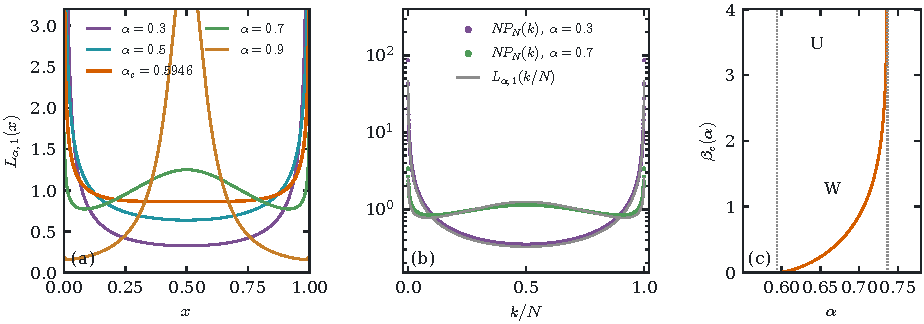
\includegraphics[width=\textwidth]{shape}
\caption{(a) The density $L_{\alpha,1}$ for $\alpha=0.3$, $0.5$, $\alpha_c$, $0.7$ and $0.9$.
At $\alpha_c$ the minimum at $1/2$ is flat to second order. (b) The exact law $NP_N(k)$ for
$N=2000$, the zeta law $f(n)\propto n^{-\alpha-1}$ for both signs and the fair start, with
$\alpha=0.3$ and $\alpha=0.7$, on a logarithmic scale, together with $L_{\alpha,1}(k/N)$. The
end values are of order $NT(N)$ and lie far above the density for $\alpha=0.3$. (c) The
threshold $\beta_c(\alpha)$ of Theorem~\ref{thm:shape} on $(\alpha_c,\alpha_1)$. Below the curve
$\La$ is W-shaped.
Section~\ref{sec:verify} describes the computations.}
\label{fig:shape}
\end{figure}

\begin{proof}
By~\eqref{eq:L-cosh}, $\La(x)=\frac{\sin\pi\alpha}\pi\phi(t)$ with $t=\log((1-x)/x)$ and
\[
 \phi(t)=\frac{1+\cosh t}{\cosh(\alpha t-\beta)+c}.
\]
The map $x\mapsto t$ is a decreasing diffeomorphism of $(0,1)$ onto $\R$, so the critical
points of $\La$ and of $\phi$ correspond, with the same type and the same order of
degeneracy. Put $s=\alpha t-\beta$ and $R(s)=\sinh s/(\cosh s+c)$, which is defined because
$\cosh s+c>0$. Then
\[
 \frac{\phi'(t)}{\phi(t)}=\tanh\frac t2-\alpha R(s)=:k(t).
\]
Since $R(s)\to\pm1$ as $s\to\pm\infty$, $k(t)\to\pm(1-\alpha)$ as $t\to\pm\infty$, so $\phi$
decreases near $-\infty$ and increases near $+\infty$. Hence the number of zeros of $k$ is
odd when they are simple, and if there are $3$ they are a minimum, a maximum and a minimum.

\emph{The function $H$.} The map $t\mapsto s$ is an increasing bijection. Let
$D=\{s:\alpha|R(s)|<1\}$. Off $D$ we have $|\alpha R(s)|\ge1>|\tanh(t/2)|$, so $k$ has no zero
there. On $D$ write $k(t)=\tanh A-\tanh B$ with $A=(s+\beta)/(2\alpha)$ and
$B=\operatorname{artanh}(\alpha R(s))$. Since $\tanh$ is increasing, $k$ has the sign of $A-B$,
that is of $\beta-H(s)$, where
\[
 H(s)=2\alpha\operatorname{artanh}(\alpha R(s))-s .
\]
So the critical points of $\La$ correspond bijectively to the solutions of $H(s)=\beta$ in
$D$. At a solution, $k'=\operatorname{sech}^2(A)(A'-B')=-\operatorname{sech}^2(A)H'(s)/(2\alpha)$ in the
variable $s$, and $\phi''=\phi k'$ there, so the critical point is nondegenerate exactly when
$H'(s)\ne0$.

\emph{The sign of $H'$.} We have $R'(s)=(1+c\cosh s)/(\cosh s+c)^2$, and with $w=\cosh s$ a
direct computation gives
\[
 2\alpha^2R'(s)-\bigl(1-\alpha^2R(s)^2\bigr)=-\frac{Q(w)}{(w+c)^2},\qquad
 Q(w)=(1-\alpha^2)(w-w_\minus)(w-w_\plus),
\]
where $w_\pm=-c\pm\alpha\sin(\pi\alpha)/\sqrt{1-\alpha^2}$ are the roots of
$(1-\alpha^2)w^2+2c(1-\alpha^2)w+c^2-\alpha^2$, whose discriminant is $4\alpha^2(1-\alpha^2)(1-c^2)$.
Since $H'(s)=[2\alpha^2R'-(1-\alpha^2R^2)]/(1-\alpha^2R^2)$ on $D$, and $w_\minus<1\le\cosh s$, we get
$H'(s)>0$ exactly when $\cosh s<w_\plus$ and $H'(s)<0$ exactly when $\cosh s>w_\plus$. With
$\sin\pi\alpha=2\sin(\pi\alpha/2)\cos(\pi\alpha/2)$ and $1+c=2\cos^2(\pi\alpha/2)$, the inequality
$w_\plus>1$ reads $\alpha\sin(\pi\alpha/2)>\cos(\pi\alpha/2)\sqrt{1-\alpha^2}$, and both sides are
nonnegative, so it is $\alpha^2>\cos^2(\pi\alpha/2)$, that is $\alpha>\alpha_c$.

\emph{The domain $D$.} The function $R$ is odd. If $c\ge0$, that is $\alpha\le1/2$, $R$ increases
on $[0,\infty)$ to the limit $1$, so $D=\R$. If $c<0$, $R$ increases on $[0,s_m]$ with
$\cosh s_m=-1/c$ to the value $R(s_m)=1/\sin\pi\alpha$, and then decreases to $1$. So $D=\R$ exactly
when $\alpha<\sin\pi\alpha$, that is $\alpha<\alpha_1$. For $\alpha\ge\alpha_1$ the set $D$ is $\R$
minus two closed intervals $\pm[s_1,s_2]$ around $\pm s_m$, which are single points when
$\alpha=\alpha_1$, and $H\to+\infty$ at both edges of $[s_1,s_2]$ and $H\to-\infty$ at both edges of
$[-s_2,-s_1]$, because $\alpha R\to1$ there from below. In every case $H$ is odd with $H(0)=0$,
and $H(s)\to\mp\infty$ as $s\to\pm\infty$, since $\alpha R\to\pm\alpha$ and $\operatorname{artanh}$ stays
bounded.

\emph{Counting.} Let $\alpha\le\alpha_c$. Then $D=\R$ and $H'<0$ except at $s=0$ when $\alpha=\alpha_c$,
so $H$ is a decreasing bijection of $\R$, and $H(s)=\beta$ has exactly one solution. It is
simple unless $s=0$ and $H'(0)=0$, that is $\alpha=\alpha_c$ and $\beta=0$. Let
$\alpha_c<\alpha<\alpha_1$. Then $D=\R$, $H'>0$ on $(-s_0,s_0)$ and $H'<0$ outside, so $H$ decreases
from $+\infty$ to a local minimum $-H(s_0)$ at $-s_0$, increases to the local maximum
$H(s_0)>H(0)=0$ at $s_0$, and decreases to $-\infty$. Hence $H(s)=\beta$ has $3$, $2$ or $1$
solutions according as $|\beta|<$, $=$ or $>H(s_0)$, all simple except the double one at
$\pm s_0$ in the case of equality. By the definition of $R$, $H(s_0)=\beta_c(\alpha)$
of~\eqref{eq:betac}, which is therefore finite and positive. Finally let $\alpha\ge\alpha_1$. On
$(0,s_1)$ the function $H$ rises from $0$ to $+\infty$, so $H'$ cannot be negative just below
$s_1$, which forces $s_0\ge s_1$ and $H'>0$ on $(-s_1,s_1)$. On $(s_2,\infty)$ it falls from
$+\infty$, which forces $s_0\le s_2$ and $H'<0$ there, and likewise on $(-\infty,-s_2)$. So each
of the three components of $D$ carries exactly one solution of $H=\beta$, all simple, for
every $\beta$. This proves (a) to (c).
\end{proof}

The monotonicity of $H$ is what closes the count. Descartes' rule for the exponential sum
that has the sign of $\phi'$ gives at most $3$ zeros only for $\alpha\le1/2$. As $\alpha$
increases to $\alpha_1$ the window $\beta_c$ opens to $\infty$, and at $b=0$ the dominated
regime of Section~\ref{sec:dominated} takes over. There the density~\eqref{eq:ratio-density}
of the ratio $Z_\minus/Z_\plus$ has an interior maximum exactly when $\alpha>\sin\pi\alpha$,
that is $\alpha>\alpha_1$, since the numerator of its logarithmic derivative in $r=y^\alpha$ is
$-(1+\alpha)r^2-2cr-(1-\alpha)$, which has a positive root exactly when $c<0$ and
$c^2>1-\alpha^2$. So the two shape thresholds meet at $\alpha_1$. Near $\alpha_c$ with $b=1$ the
two minima split off from $1/2$ like a pitchfork, at distance
$\frac14(3(2\alpha^2-1-\cos\pi\alpha)/(\alpha^2(1-\alpha^2)))^{1/2}(1+o(1))$ from $1/2$, which
follows from the expansion $\chi(t)=\chi(0+)+\frac13\alpha^2(1-\alpha^2)t^2(1+O(t^2))$ of the
function $\chi(t)=\cosh\alpha t+c-\alpha\sinh(\alpha t)\coth(t/2)$ that has the sign of $k$ for
$b=1$. At $\alpha=1/2$ and $b=1$ the theorem gives the arcsine density, with its minimum at
$1/2$.

\subsection{Difference forms of the renewal theorem}\label{sec:dsrt}

The end profiles are renewal mass functions. To compare neighbouring values of $P_N$ near an
end we need the differences of $u_\sgn$, and (DSRT$_\sgn$) asks that they have the size of
the derivative of $\frac{\sin\pi\alpha}\pi/(nT_\sgn(n))$. It holds for log-convex laws.

\begin{lemma}[the difference renewal theorem for log-convex laws]\label{lem:dsrt}
Let $f$ be a log-convex mass function on $\{1,2,\dots\}$ with $f(1)>0$ and a tail $T$ that is
regularly varying with index $-\alpha\in(-1,0)$. Then $f$ satisfies (LB) and (SRT), its renewal
mass function $u$ is strictly decreasing, and $u(j)-u(j+1)\sim(1-\alpha)u(j)/j$.
\end{lemma}

\begin{proof}
A log-convex $f$ that tends to $0$ is nonincreasing, so $f(n)\le2T(n/2)/n\le CT(n)/n$, which is
(LB), and Doney's theorem (Lemma~\ref{lem:cd}(iii)) gives (SRT), so $u$ is regularly varying
with index $\alpha-1$. By de Bruijn and Erd\H{o}s~\cite[Theorem~1]{debruijnerdos1953}, $u$ is
log-convex, so $r_j=u(j+1)/u(j)$ is nondecreasing, and $r_j<1$ because $u\to0$. For $\lambda>1$
and $i$ large put $j=\lfloor i/\lambda\rfloor$. Then
$\log u(i)-\log u(j)=\sum_{l=j}^{i-1}\log r_l$ lies between $(i-j)\log r_j$ and $(i-j)\log r_i$,
and tends to $(\alpha-1)\log\lambda$. Since $i-j\sim(\lambda-1)i/\lambda$, this gives
$\limsup_ii\log r_i\le(\alpha-1)\lambda\log\lambda/(\lambda-1)$, and applying the other inequality
with $i$ in place of $j$ gives $\liminf_jj\log r_j\ge(\alpha-1)\log\lambda/(\lambda-1)$. Let
$\lambda\downarrow1$. So $j\log r_j\to\alpha-1$, which is the claim.
\end{proof}

For Sibuya laws, $T(n)=\prod_{i<n}(1-\alpha/i)$, one has $r_j=(j+\alpha)/(j+1)$ exactly. The zeta
law $f(n)=n^{-\alpha-1}/\zeta(\alpha+1)$ is strictly log-convex. We do not know whether
(LR) and the first-difference condition $|f(n)-f(n+1)|=O(f(n)/n)$ imply (DSRT) when
$\alpha\le1/2$.

We also need the end profile of a prepared start. For an initial run $(\nu_\plus,\nu_\minus)$ with
$n\nu_\pm(n)\to0$, Theorem~\ref{thm:initial}(f) gives $P_N(N-j)/T_\plus(N)\to\kappa_\plus(j)$ for
$j\ge1$, with $\kappa_\plus$ as in~\eqref{eq:kappa-prep}, and we write
$\widetilde\kappa_\plus=(\widetilde\kappa_\plus(0),\kappa_\plus(1),\kappa_\plus(2),\dots)$ for the
profile with the end value $\widetilde\kappa_\plus(0)=\lim_NQ_\plus(N)/T_\plus(N)$, when this limit
exists in $[0,\infty]$. We say that the initial run satisfies (S) if
\begin{equation}\label{eq:S}\tag{S}
 |\nu_\sgn(n+1)-\nu_\sgn(n)|=o(n^{-2}),\qquad
 |\nu_\sgn(n+1)-2\nu_\sgn(n)+\nu_\sgn(n-1)|=o(n^{-3})
\end{equation}
for both signs, and the limits $\widetilde\kappa_\pm(0)$ exist. Fresh and fair starts satisfy (S)
under (LR) and (LD2), and so does every smooth regularly varying $\nu$, such as
$\nu(n)\propto n^{-1-\gamma}$ for any $\gamma>0$.

\begin{lemma}[the prepared profile]\label{lem:prep-profile}
Assume (BAL), (SPAN), (DSRT$_\minus$) and the first half of (S) for $\nu_\minus$. Then
$\kappa_\plus(j+1)-\kappa_\plus(j)=(1+o(1))(u_\minus(j+1)-u_\minus(j))$. In particular
$\widetilde\kappa_\plus$ is eventually strictly decreasing.
\end{lemma}

\begin{proof}
Write $u=u_\minus$, $\Delta u(i)=u(i+1)-u(i)$ and $\Delta u(0)=u(1)-1$. From~\eqref{eq:kappa-prep},
$\Delta\kappa_\plus(j)=\pi_\plus\Delta u(j)+\sum_{d\le j}\nu_\minus(d)\Delta u(j-d)+\nu_\minus(j+1)$. The
part $d\le j/2$ is $(\pi_\minus+o(1))\Delta u(j)$ by dominated convergence, since $\Delta u$ is
regularly varying by (DSRT$_\minus$). With $\sum_{i<j/2}\Delta u(i)=u(\lceil j/2\rceil)-1$, the rest
is $\sum_{0\le i<j/2}(\nu_\minus(j-i)-\nu_\minus(j+1))\Delta u(i)+\nu_\minus(j+1)u(\lceil j/2\rceil)$. With
$\delta_j=\sup_{n\in[j/2,j+1]}|\Delta\nu_\minus(n)|=o(j^{-2})$ and
$\sum_{i\le j}(i+1)|\Delta u(i)|\le Cju(j)$, this is at most $C\delta_jju(j)+o(1/j)u(j/2)=o(u(j)/j)$,
while $|\Delta u(j)|\sim(1-\alpha)u(j)/j$.
\end{proof}

\subsection{Sign changes of the discrete law}\label{sec:signs}

For a finite or infinite real sequence $(s_i)$ let $V(s)$ be the number of sign changes of
the sequence of its nonzero terms. The sign changes of $k\mapsto P_N(k+1)-P_N(k)$ are the
strict local extrema of $P_N$ when no two neighbouring values are equal.

\begin{theorem}[a lower bound on the sign changes]\label{thm:signs}
Assume (BAL), (SPAN) and (SRT$_\pm$), and let the initial run be such that
$NP_N(k)=\La(k/N)+o(1)$ uniformly on compact subsets of $(0,1)$ (for instance a fresh
start, or under (LB$_\pm$) any initial run with $n\nu_\pm(n)\to0$) and such that
$W^\pm_N=o(T_\pm(N))$. Assume that the limits $\widetilde\kappa_\pm(0)$ exist and are finite,
that $\widetilde\kappa_\pm(j+1)\ne\widetilde\kappa_\pm(j)$ for all $j\ge0$, and that
$\widetilde\kappa_\pm$ is strictly decreasing from some point on. Let
$\sigma_\pm=V((\widetilde\kappa_\pm(j+1)-\widetilde\kappa_\pm(j))_{j\ge0})$, and let $\sigma_L$ be the
number of critical points of $\La$, which is $1$ or $3$ by Theorem~\ref{thm:shape}, each of
them a strict local extremum. Then for all large $N$,
\[
 V\bigl((P_N(k+1)-P_N(k))_{0\le k<N}\bigr)\ge\sigma_L+\sigma_\plus+\sigma_\minus .
\]
\end{theorem}

\begin{proof}
If $(s_{i_l})$ is a subsequence of $(s_i)$, the differences of $(s_i)$ have at least as many
sign changes as the differences of $(s_{i_l})$, since each nonzero difference
$s_{i_{l+1}}-s_{i_l}$ is a sum of consecutive differences of $(s_i)$, one of which has its
sign. Let $c_1<\dots<c_s$ be the critical points of $\La$, $s=\sigma_L$. Since $\La\to\infty$ at
both ends, $\La$ decreases strictly on $(0,c_1]$ and increases strictly on $[c_s,1)$, and the
critical points alternate between strict minima and strict maxima, starting and ending with
a minimum. Choose $z_0\in(0,c_1)$ and $z_{s+1}\in(c_s,1)$. The differences of
$\La(z_0),\La(c_1),\dots,\La(c_s),\La(z_{s+1})$ have the signs $-,+,-,\dots,+$, with $s$ sign
changes. Choose $J$ such that $\widetilde\kappa_\plus$ and $\widetilde\kappa_\minus$ are strictly
decreasing on $[J-1,\infty)$, so $\widetilde\kappa_\pm(J)>0$. Consider the subsequence of
$(P_N(k))_{0\le k\le N}$ at the points
\[
 0,1,\dots,J,\ \lfloor z_0N\rfloor,\lfloor c_1N\rfloor,\dots,\lfloor c_sN\rfloor,\lfloor z_{s+1}N\rfloor,\ N-J,\dots,N .
\]
By Theorem~\ref{thm:initial}(f), its mirror, and the definition of $\widetilde\kappa_\pm(0)$,
$P_N(N-j)/T_\plus(N)\to\widetilde\kappa_\plus(j)$ and $P_N(j)/T_\minus(N)\to\widetilde\kappa_\minus(j)$ for
$0\le j\le J$. Since consecutive values of $\widetilde\kappa_\pm$ differ, for large $N$ the
differences at the two ends have the signs of the differences of $\widetilde\kappa_\pm$, with
$\sigma_\minus$ and $\sigma_\plus$ sign changes, and the differences next to $j=J$ have the sign
of $\widetilde\kappa_\pm(J)-\widetilde\kappa_\pm(J-1)<0$. In the bulk, $NP_N(\lfloor zN\rfloor)\to\La(z)$ at
each chosen point, so for large $N$ the bulk differences have the signs $-,+,\dots,+$ with $s$
sign changes. At the junctions, $P_N(J)\sim T_\minus(N)\widetilde\kappa_\minus(J)$ and
$P_N(N-J)\sim T_\plus(N)\widetilde\kappa_\plus(J)$, while the bulk values are $O(1/N)$ and
$NT_\pm(N)\to\infty$. So the difference from $P_N(J)$ to $P_N(\lfloor z_0N\rfloor)$ is negative and
the difference from $P_N(\lfloor z_{s+1}N\rfloor)$ to $P_N(N-J)$ is positive. Reading from left to
right, the last difference at the minus end, the junction and the first bulk difference are
all negative, and the last bulk difference, the junction and the first difference at the plus
end, which is $\sim T_\plus(N)(\widetilde\kappa_\plus(J-1)-\widetilde\kappa_\plus(J))$, are all positive.
So the junctions add no sign change, and the subsequence has $\sigma_\minus+s+\sigma_\plus$ sign
changes.
\end{proof}

\begin{example}[the fair start and the fresh start]\label{ex:counts}
Let both run laws be the zeta law, so $b=1$, and let the start be fair. Then
$Q_\pm(N)=\frac12T(N)$, so $\widetilde\kappa_\pm(0)=\frac12$, and~\eqref{eq:kappa-prep} gives
$\kappa_\pm(j)=\frac12u(j)+\frac12\sum_{d\le j}f(d)u(j-d)=u(j)$ for $j\ge1$. Since $u$ is strictly
decreasing by Lemma~\ref{lem:dsrt}, $\sigma_\pm=1$ if $u(1)=f(1)>\frac12$ and $\sigma_\pm=0$ if
$f(1)<\frac12$. Now $f(1)=1/\zeta(1+\alpha)$, and $\zeta(1.7)=2.054\ldots$ and
$\zeta(1.9)=1.750\ldots$. So Theorems~\ref{thm:signs} and~\ref{thm:shape} give at least $1$
sign change for $\alpha=0.3$ and $\alpha=0.5$, at least $3$ for $\alpha=0.7$, and at least
$3+1+1=5$ for $\alpha=0.9$. For a fresh plus start with different laws,
$\widetilde\kappa_\plus=(1,u_\minus(1),\dots)$ is strictly decreasing and
$\widetilde\kappa_\minus=(0,u_\plus(1),u_\plus(2),\dots)$ has one sign change, so the bound is
$\sigma_L+1$.
\end{example}

\subsection{The exact count}\label{sec:count}

In every case of Section~\ref{sec:verify} with a fresh, a fair or a smooth start, the computed
number of sign changes equals the lower bound of Theorem~\ref{thm:signs} for all large $N$.
Two difference statements turn the bound into an equality. We state them as hypotheses and
prove the count from them. For a fresh plus start put $D_N(j)=P_N(N-j-1)-P_N(N-j)$.
\begin{itemize}[leftmargin=4em,labelsep=0.8em]
\item[(L)] (The layer.) For every $\eta>0$ there are $\varepsilon>0$ and $J$ such that for all large
$N$ and $J\le j\le\varepsilon N$, $|D_N(j)-T_\plus(N)(u_\minus(j+1)-u_\minus(j))|\le\eta\,T_\plus(N)u_\minus(j)/j$,
and the mirror at the minus end.
\item[(B)] (The bulk.) Uniformly for $k/N$ in compact subsets of $(0,1)$,
$N^2(P_N(k+1)-P_N(k))\to\La'(k/N)$ and $N^3(P_N(k+1)-2P_N(k)+P_N(k-1))\to\La''(k/N)$.
\end{itemize}

\begin{proposition}[the exact count]\label{prop:count}
Assume (BAL), (SPAN), (LR), (LD2) and (DSRT$_\pm$), let the start be fresh or fair, assume
that $(\alpha,b)$ is not one of the degenerate pairs of Theorem~\ref{thm:shape}(c), and assume
(L) and (B). Let $J_\pm$ be such that $\widetilde\kappa_\pm$ is strictly decreasing on $[J_\pm,\infty)$,
assume $\widetilde\kappa_\pm(j+1)\ne\widetilde\kappa_\pm(j)$ for $j<J_\pm$, and let $M_\pm$ be the number
of local maxima of $\widetilde\kappa_\pm$. Let $m_L\in\{0,1\}$ be the number of interior maxima of
$\La$. Then for all large $N$, $P_N$ has exactly $M_\plus+M_\minus+m_L$ modes, $M_\plus$ of them
within $J_\plus$ of $N$, $M_\minus$ within $J_\minus$ of $0$, and the interior one, when
$m_L=1$, at $(x_{\max}+o(1))N$ with $x_{\max}$ the maximum of $\La$. Between the end blocks
lie exactly $1+m_L$ further local minima, at $(c+o(1))N$ for the minima $c$ of $\La$, and
no antimode in the layers. For strictly log-convex run laws $M_\plus=M_\minus=1$, so the count
is $2+m_L$.
\end{proposition}

\begin{proof}
We check the sign of $\Delta P_N(k)=P_N(k+1)-P_N(k)$ on five ranges. For $0\le j<J_\plus$,
Theorem~\ref{thm:initial}(f) gives $D_N(j)$ the sign of $\widetilde\kappa_\plus(j+1)-\widetilde\kappa_\plus(j)$,
since $n\nu_\pm(n)\to0$ for fresh and fair starts. For $J_\plus\le j\le\varepsilon N$, (L) and
(DSRT$_\minus$) give $D_N(j)<0$ once $\eta<1-\alpha$, so $P_N$ increases strictly toward the plus
end through the layer. By (B) and Theorem~\ref{thm:shape}, on $[\varepsilon N,(1-\varepsilon)N]$ the sign
of $\Delta P_N(k)$ is that of $\La'(k/N)$ away from the critical points, and near each critical
point $c$ the second difference has the sign of $\La''(c)\ne0$, so $\Delta P_N$ is strictly
monotone on a window of width $\delta N$ around $cN$ and changes sign exactly once there.
The minus end is the mirror. Taking $\varepsilon$ below the first critical point and above $1$
minus the last one makes the ranges overlap, and the signs agree on the overlaps, since
$\La'>0$ near $1$ and $D_N<0$ in the plus layer. Reading the signs of $\Delta P_N$ from $k=0$
to $k=N$, the pattern is that of the minus profile, then a block of negative signs, then the
bulk block, which is empty when $m_L=0$ and $(+)^{a}(-)^{b}$ when $m_L=1$, then a block of
positive signs, then the mirror of the plus profile. The modes are the changes from $+$ to
$-$, a leading $-$ and a trailing $+$, which gives $M_\minus+m_L+M_\plus$, and the minima are
the changes from $-$ to $+$, which are the minima of $\La$. For log-convex laws $u_\mp$ is
strictly decreasing with limit $0$, and the profiles $(1,u(1),\dots)$, $(0,u(1),\dots)$ and
$(\frac12,u(1),\dots)$ have one local maximum each, at $j=0$ or $j=1$ according as $u(1)$ is
below or above the end value, with no tie when $f(1)\ne\frac12$ for the fair start.
\end{proof}

What is proved toward (L) and (B). Lemma~\ref{lem:prep-profile} and
Theorem~\ref{thm:initial}(f) give the first range for every start with (S). For (L), the
decomposition of $D_N(j)$ by the fresh identity into four sums, as in the first-difference
theorem of~\cite[Section~6]{paperF}, reduces it to a difference form of Doney's local bound,
$|V_m(n-1)-V_m(n)|\le Cmf(n)/n$ for all $m\ge1$ and $n\ge a_m$ with $V_m=f^{*m}$, under (SPAN),
(LR) and the first-difference condition. This is the case $\alpha<1$ of the difference form
of the local big-jump theorem of~\cite[Section~6]{paperF}, with no centering, and we have not
written its proof. For (B),
the first-difference limit follows by taking a difference inside the proof of
Theorem~\ref{thm:local}, and the second-difference limit is the part that needs work: the range
of few runs contributes at the order $N^{-3}$ through the second differences of the convolution
powers. The computations of Section~\ref{sec:verify} agree with (L), (B) and the count in every
case.

\ifarxivbuild
\begin{remark}[a conjecture that fails]\label{rem:oscillating}
An earlier version of this paper conjectured that under the hypotheses of
Theorem~\ref{thm:signs}, (LB$_\pm$), the first-difference condition and strictly log-convex
run laws, the lower bound is an equality for all large $N$. It is not, because the hypotheses
of Theorem~\ref{thm:signs} put no smoothness on the initial run. Take Sibuya laws for both
signs and an initial plus run with $\nu_\plus(n)=c\,n^{-1-\alpha}(1+0.9(-1)^n)$ for $n\ge2$ and the
rest of the mass at $d=1$. Then $n\nu_\plus(n)\to0$, $Q_\plus(N)/T(N)$ converges, and $\kappa_\minus$
is eventually strictly decreasing, so every hypothesis holds. The alternating part of
$\nu_\plus$ enters $P_N(k)$ through $\nu_\plus(k)T_\minus(N-k)$ and the near-diagonal terms, with
an amplitude of order $N^{-1-2\alpha}$ that does not cancel, and it beats the slope of
$\La(k/N)/N$ near every critical point. For $\alpha=0.7$ the exact law has $31$, $35$, $50$ and
$62$ modes at $N=500$, $1000$, $2000$ and $3000$, and for $\alpha=0.3$ with
$\nu_\plus(n)=c(n^{-1-\alpha}+0.3(-1)^nn^{\alpha-2})$ it has $54$, $110$, $223$ and $338$. The
condition (S) excludes these starts, and the count of Proposition~\ref{prop:count} holds
for them in no form. At the degenerate point $\alpha=\alpha_c$, $b=1$, the count depends on the
law: with the fair start the Sibuya law has $3$ modes and the zeta law $2$ at every computed
$N\le3000$, so the nondegeneracy hypothesis cannot be dropped.
\end{remark}
\fi

\section{Open problems}\label{sec:open}

We list what the paper leaves open, in the order of the sections.
\begin{enumerate}[(1)]
\item (The lower half of the matching.) Theorem~\ref{thm:ends}(b) matches the end layer to the
bulk uniformly under (LB$_\plus$). Lemma~\ref{lem:E} gives its upper half under (SRT$_\pm$) for
$\alpha\ne1/2$. Whether the lower half holds under (SRT$_\pm$) alone is open
(Remark~\ref{rem:M0}).
\item (Necessity in the aged law.) Theorem~\ref{thm:local} needs (SRT$_\pm$) for a fresh start.
In the aged decomposition the plus part sees $F^\minus_{N-d}(k-d)$ with the same number
$N-k$ of minus steps for every $d$, so we expect a failure of (SRT$_\minus$) to survive the
average over $d$ and break Theorem~\ref{thm:aging}(a). This is not proved. Whether (SRT$_\pm$)
alone implies (U) when $\alpha\le1/2$, the uniform matching of the aged layer to $L_\theta$,
and the slowly varying factor at $\alpha=1/2$ are open as well.
\item (The line $\alpha_\minus=1/2$.) The uniform matching of Theorem~\ref{thm:dominated}(d) is
stated for $\alpha_\minus\ne1/2$. On the line, both routes of the proof lose a ratio of slowly
varying factors of $T_\minus$, which need not be bounded.
\item (The big-jump zone of the dominated regime.) Between the bulk at the scale $D_N$ and the
lighter end we expect the two-term kernel of~\cite{paperF} with the signs exchanged, and a
window of width $(\log N)^{1-\alpha_\plus}D_N$ when the lighter mean is finite. Nothing is proved
there, and the initial-run theorem of the dominated regime is written only for minus initial
runs (Remark~\ref{rem:dom-initial}).
\item (The exact count.) Proposition~\ref{prop:count} rests on the hypothesis (B), a
first- and second-difference local limit theorem in the bulk. The first-difference half follows
from the proof of Theorem~\ref{thm:local}. The second-difference half needs a second-difference
form of Lemma~\ref{lem:Lstar} on the range of few runs. The count in the dominated regime
is open as well. We expect $M_\plus+M_\minus+m$ modes there, with $m=1$ exactly when the density
$\rho$ has an interior maximum, which for $\mu_\minus<\infty$ is $\alpha_\plus>1/2$, and the
threshold curve in the $(\alpha_\plus,\alpha_\minus)$ square runs from $(\alpha_1,\alpha_1)$ to
$(1/2,1)$. Every exact law we computed agrees with this.
\item (Every $N$.) All counts here are for large $N$. For completely monotone run laws with a
fresh start, every exact law we computed has at most $3$ local maxima in $\{1,\dots,N-1\}$ for
every $N$. For the fair start no such bound holds: there are completely monotone laws, the
same for both signs, whose fair law has $5$ modes at $N=39$ while both fresh laws are
monotone. We know no proof of a bound for every $N$.
\item (The line $\alpha=1$.) When one or both indices equal $1$ the periods may or may not have
a finite mean, and the scales carry slowly varying corrections. The local tools of
Berger~\cite{berger2019ptrf} for the Cauchy domain should give the local law at the scale
$N\ell(N)/m(N)$, with $m$ the truncated mean, and the dominated regime with a lighter law of
index $1$ converges at the rate $1/\log N$. We have not worked out either line.
\end{enumerate}

\section{Computations}\label{sec:verify}

No proof uses a computed number. The computations check the exact identities and test
the theorems at moderate $N$. Except where we say otherwise they use the zeta law
$f(n)=n^{-\alpha-1}/\zeta(\alpha+1)$ for both signs, so $b=1$, and the fair start. The
exact law comes from~\eqref{eq:run-sum}, or from the first-run decomposition with the
convolution powers computed by FFT. Every entry is a sum of nonnegative terms, so the
relative rounding error stays small, and the total mass is $1$ to $12$ digits in every
case. The identities of Section~\ref{sec:identities} and~\eqref{eq:run-sum} agree with a sum
over all sign strings for $N\le12$, for two different laws of the two signs and a general
initial run, to $2\cdot10^{-16}$, and the aged law of Section~\ref{sec:aged} agrees with a sum
over all run sequences for $t_a+N\le12$ to $6\cdot10^{-16}$.

\emph{The local law and the ends.} Table~\ref{tab:ratios} shows the ratio
$NP_N(k)/L_{\alpha,1}(k/N)$ at $k=N/2$ and $k=N/20$, and the number of sign changes of
$k\mapsto P_N(k+1)-P_N(k)$. At $\alpha=1/2$ the central ratio is $1.0149$, $1.0105$ and $1.0075$
for $N=1000$, $2000$ and $4000$, and the distance to $1$ shrinks by a factor close to
$\sqrt2$ when $N$ doubles. The convergence is slower away from $\alpha=1/2$ and much slower
as $\alpha\to1$. The sign changes sit at $k=N/2$ for $\alpha\le0.58$. At $\alpha=0.7$ and
$N=1000$ they sit at $k=104$, $500$ and $896$, near the minima of $L_{0.7,1}$. At
$\alpha=0.9$ and $N=4000$ they sit at $k=1$, $142$, $2000$, $3858$ and $3999$, and the two
outer ones come from the ends, as in Example~\ref{ex:counts}. On both sides of $\alpha_c$ the
count is $1$ at $\alpha=0.58$ and $3$ at $\alpha=0.61$. Every count in the table equals the
lower bound of Theorem~\ref{thm:signs}. At the plus end, for $\alpha=1/2$, the ratio
$P_N(N-j)/(T(N)u(j))$ lies in $[1.0009,1.0040]$ for $1\le j\le5$ at $N=1000$ and in
$[1.0004,1.0020]$ at $N=2000$, and the ratio of $P_N(N-j)$ to $T(N)u(j)\Phi_1(j/N)$ over
$1\le j\le0.8N$ lies in $[1.0004,1.0148]$ at $N=1000$ and in $[1.0002,1.0105]$ at $N=2000$, as
Theorem~\ref{thm:ends}(b) predicts. For unequal laws, the zeta law for the plus runs and
$f_\minus(n)\propto(n+3)^{-\alpha-1}$ for the minus runs with a fresh plus start, the ratios to
$L_{\alpha,b}$ at $x=0.1,0.3,\dots,0.9$ lie in $[1.0121,1.0397]$ at $N=1000$ and in
$[1.0069,1.0199]$ at $N=4000$ for $\alpha=1/2$, where $b=2.4498$.

\begin{table}[t]
\centering
\begin{tabular}{@{}cccccc@{}}
\toprule
$\alpha$ & $N$ & ratio at $k=N/2$ & ratio at $k=N/20$ & sign changes \\
\midrule
$0.3$ & $1000$, $2000$, $4000$ & $1.0852$, $1.0687$, $1.0555$ & $1.1023$, $1.0845$, $1.0694$ & $1$, $1$, $1$\\
$0.5$ & $1000$, $2000$, $4000$ & $1.0149$, $1.0105$, $1.0075$ & $1.0045$, $1.0036$, $1.0028$ & $1$, $1$, $1$\\
$0.58$ & $1000$, $2000$, $4000$ & $0.9846$, $0.9863$, $0.9883$ & $1.0142$, $1.0114$, $1.0090$ & $1$, $1$, $1$\\
$0.61$ & $1000$, $2000$, $4000$ & $0.9696$, $0.9739$, $0.9781$ & $1.0282$, $1.0230$, $1.0185$ & $3$, $3$, $3$\\
$0.7$ & $1000$, $2000$, $4000$ & $0.9023$, $0.9159$, $0.9285$ & $1.1202$, $1.1004$, $1.0833$ & $3$, $3$, $3$\\
$0.9$ & $1000$, $2000$, $4000$ & $0.4903$, $0.5168$, $0.5433$ & $2.2892$, $2.1277$, $1.9905$ & $5$, $5$, $5$\\
\bottomrule
\end{tabular}
\caption{The ratio $NP_N(k)/L_{\alpha,1}(k/N)$ and the number of sign changes of the first
differences of $P_N$, for the zeta law and the fair start.}
\label{tab:ratios}
\end{table}

\emph{The initial run.} For $\alpha=1/2$, a fair sign and $\nu_\pm(d)=d^{-1.2}/(2\zeta(1.2))$,
the central ratio is $0.815$, $0.836$ and $0.855$ for $N=500$, $1000$ and $2000$. The gap to
$1$ decays like $N^{-0.2}$, the order of $\Prob(D\ge N)$, which enters through the first run
with $\varepsilon N\le D<N$ in the proof of Theorem~\ref{thm:initial}(a). For $D$ uniform on
$\{1,\dots,N/2\}$ with a fair sign, $NP_N(k)$ at $k/N=0.3$ and $0.5$ is $0.898$ and $1.325$ at
$N=500$ and $0.884$ and $1.299$ at $N=2000$, against the values $0.8694$ and $1.2732$ of the
mixture~\eqref{eq:mixture} with $\rho_\pm=1$ on $(0,\frac12)$ and $\pi^0=0$, and against the
values $0.6946$ and $0.6366$ of $L_{1/2,1}$ for a fresh start.

\emph{The aged law.} For Theorem~\ref{thm:aging} with $\theta\in\{\frac12,1,2\}$ and
$N=500$, $1000$, $2000$, the aged law is computed from the first-run decomposition with the
initial run~\eqref{eq:aged-law}. At $\alpha=1/2$ and $\theta=1$ the largest relative error of
$NP_N(\lfloor xN\rfloor)$ against $L_\theta(x)$ on $x\in[0.1,0.9]$ is below $5\%$ at $N=2000$ and
decreases with $N$, and at $\alpha=0.7$ it is below $15\%$. The atom $P_N(N)$ is $1.0282$,
$1.0198$ and $1.0139$ times $Q^\infty_\plus(1)$ at the three values of $N$ for $\alpha=1/2$, and
$1.0418$, $1.0293$ and $1.0206$ times $Q^\infty_\plus(\frac12)$. The ratio
$P_N(N-j)/(T_\plus(N)c_\plus(\theta)u_\minus(j))$ for $j=1,\dots,5$ lies in $[1.050,1.089]$ at
$N=2000$ for $\theta=1$, and after removal of the term $T_\plus(N)\sum_{d\le j}\nu_\minus(d)u_\minus(j-d)$,
which is $o(T_\plus(N))$ but only by a factor of order $1/(NT(N))$, it lies in $[1.0161,1.0167]$.
Each deviation shrinks by about $1/\sqrt2$ per doubling of $N$. The mass identity
$\int_0^1L_\theta+Q^\infty_\plus+Q^\infty_\minus=1$ and the closed forms of $Q^\infty_\sgn$ and
$c_\sgn$ agree with quadrature to $10$ digits.

\emph{The dominated regime.} For Theorem~\ref{thm:dominated} we take zeta laws with a fresh
plus start, $N=1000$, $2000$, $4000$, the mixed pair $(\alpha_\plus,\alpha_\minus)=(0.6,1.5)$ and
the infinite pair $(0.5,0.8)$. The largest relative error of $D_NP_N(N-j)$ against
$\rho(j/D_N)$ on $y\in[0.05,1]$ is $0.304$, $0.247$ and $0.201$ in the mixed case, decreasing
like $N^{-0.3}$, and on $y\in[0.1,3]$ it is $0.588$, $0.533$ and $0.478$ in the infinite case,
where the lighter sums carry a drift correction of relative size $m^{1-1/\alpha_\minus}$ with
only about $83$ cycles at $N=4000$. The finite-$N$ main term of the proof,
$T_\plus(N-j)\sum_mu^\minus_m(j)\phi(mT_\plus(N-j))$, is closer, within $0.098$ and $0.078$ at
$N=4000$. At the plus end the ratio $P_N(N-j)/(T_\plus(N)u_\minus(j))$ for $j\le5$ lies in
$[1.0000,1.0172]$ and $[1.0000,1.0003]$ at $N=4000$, and at the minus end
$P_N(i)/(T_\minus(N)u_\plus(i))$ for $1\le i\le5$ is within $0.9\%$ of $1$ in both cases. In the
mixed case the law has exactly $3$ modes at every $N$, at $k=1$, at $k=N$ and at an interior
point near $N-y^*D_N$ with $y^*$ the maximum of $\phi$, since $\alpha_\plus>1/2$; for
$(\alpha_\plus,\alpha_\minus)=(0.4,1.5)$ it has exactly $2$, at $k=1$ and $k=N$. At $\alpha=1/2$ the
density $\phi$ agrees with $e^{-\pi x^2/4}$ to $8$ digits, and the ratio density at
$\alpha=0.7$ agrees with~\eqref{eq:ratio-density} to $10$ digits.

\emph{The shape.} The roots are $\alpha_c=0.594611644056836$ and
$\alpha_1=0.736484448241517$. On a grid of $\alpha$ from $0.02$ to $0.98$ and $|\beta|\le6$ in
steps of $0.05$, the number of zeros of the exponential sum that has the sign of
$\frac d{dt}\log\La$ agrees with Theorem~\ref{thm:shape}, and it flips between
$\beta_c(0.7)-10^{-3}$ and $\beta_c(0.7)+10^{-3}$. The transform~\eqref{eq:stieltjes} agrees with
direct quadrature in $30$-digit arithmetic, and at $\alpha=1/2$ the double
integral~\eqref{eq:Lambda} agrees with $L_{1/2,1}$ to a relative error below $10^{-13}$ at
$x=0.2$, $0.5$ and $0.7$. For Proposition~\ref{prop:count} we use Sibuya laws,
$T(n)=\prod_{i<n}(1-\alpha/i)$, which are log-convex, and $N=250,500,\dots,3000$. With $b=1$ and
a fresh plus or a fair start the law has exactly $2$ modes at every $N$ for $\alpha=0.3$ and
$0.5$, and exactly $3$ for $\alpha=0.65$, $0.7$ and $0.9$, with the bulk minima at $0.136N$,
$0.085N$ and $0.021N$ against the minima $0.1388$, $0.085$ and $0.0216$ of $\La$. For the law
$f(n)\propto n^{-1.7}$ on $n\ge2$ the profiles have maxima at $j=0,2,4$ and the counts are $6$
for the fresh plus start and $7$ for the fair start at every $N$. For unequal tails of the
same index, the minus law a mixture of a Sibuya law and a geometric law so that $b=0.6$ at
$\alpha=0.7$, inside the window, the count is $3$ at every $N$; for $b=0.5$ at $\alpha=0.65$,
outside the window, it is $3$ up to $N=1500$ and $2$ from $N=2000$ on; and for $b=0.25$ at
$\alpha=0.7$ it is still $3$ at $N=3000$, where the local law itself is far from its limit
because the light component adds $O(N^\alpha)$ steps of finite mean. For (L), the ratio
$D_N(j)/(T_\plus(N)(u_\minus(j+1)-u_\minus(j)))$ at $j=5$, $20$, $50$ and $N=3000$ is $0.952$,
$0.897$, $0.847$ for $\alpha=0.3$ and $0.969$, $0.917$, $0.819$ for $\alpha=0.7$, rising with $N$ at
fixed $j$. For (B), $N^2(P_N(k+1)-P_N(k))$ at $x=0.2$, $0.3$, $0.4$, $0.45$ and $N=3000$ is
$-1.688$, $-0.681$, $-0.266$, $-0.125$ against $\La'=-1.571$, $-0.635$, $-0.248$, $-0.117$ for
$\alpha=0.3$, and $1.435$, $1.729$, $1.261$, $0.697$ against $1.413$, $1.681$, $1.208$, $0.666$
for $\alpha=0.7$. The scans decide signs from the floating-point differences, whose smallest
relative gap at a counted extremum was $7\cdot10^{-10}$ against a rounding error of order
$10^{-13}$.

The scripts and their outputs, each headed by the hash of its script, are in the folder
\nolinkurl{kagey-problems/problem131/paperG} of \url{https://github.com/apemm/Kagey-Problems}.
The command \texttt{python -I verify\_all.py} runs the main checks in a few minutes, and
\nolinkurl{README.md} lists what each script tests and how to run the longer scans.


\appendix
\section{Routine facts}\label{app:routine}

This appendix proves the routine facts used in Sections~\ref{sec:setting} to~\ref{sec:local}.

\subsection{Regular variation}

\begin{lemma}\label{lem:rv-facts}
Let $T$ be regularly varying with index $-\alpha\in(-1,0)$, nonincreasing and positive.
\begin{enumerate}[(i)]
\item (R4) of Section~\ref{sec:rv} holds.
\item If $a$ is increasing with $tT(a(t))\to1$, then $\sup_{m\ge1}mT(a_m)<\infty$.
\item With $m_N(t)=\lfloor t/T(N)\rfloor$, $a_{m_N(t)}/N\to t^{1/\alpha}$ uniformly for $t$ in compact
subsets of $(0,\infty)$.
\end{enumerate}
\end{lemma}

\begin{proof}
(i) The function $\phi(w)=wT(w)$ is regularly varying with index $1-\alpha>0$, and it is
positive, so $\inf_{w\ge1}\phi(w)>0$ because $\phi(w)\to\infty$. By Potter's
theorem~\cite[Theorem~1.5.6]{bgt1989} there is
$x_0$ with $\phi(y)/\phi(x)\le2(y/x)^{(1-\alpha)/2}$ for $x_0\le y\le x$. By (R2),
$2^lT(2^{l-1})\le C\phi(2^l)$. The terms with $2^l\ge x_0$ add up to at most
$C\phi(x)\sum_{l\ge0}2^{-l(1-\alpha)/2}$, and the finitely many terms with $2^l<x_0$ add up to a
constant, which is at most $C\phi(x)$. For the second sum let $x\ge x_0$. The first term
with $2^l>x$ has $2^{l-1}\in(x/2,x]$, so it is at most $T(x/2)\le CT(x)$ by (R2). The later
terms have $2^{l-1}\ge x$, and Potter's bounds give $T(y)/T(x)\le2(y/x)^{-\alpha/2}$ for
$y\ge x\ge x_0$. So the sum is at most $CT(x)\sum_{l\ge0}2^{-l\alpha/2}$. For $1\le x<x_0$ the sum is at most
$\sum_{l\ge1}T(2^{l-1})<\infty$, which is at most $CT(x_0)\le CT(x)$.

(ii) The sequence $mT(a_m)$ converges to $1$ and each term is finite.

(iii) Fix $t>0$ and write $m=m_N(t)$. Then $mT(N)\to t$ and $mT(a_m)\to1$, so
$T(a_m)/T(N)\to1/t$. Take a subsequence along which $a_m/N\to\lambda\in[0,\infty]$. If
$\lambda\in(0,\infty)$, (R1) gives $T(a_m)/T(N)\to\lambda^{-\alpha}$, so $\lambda=t^{1/\alpha}$. If
$\lambda=0$ or $\lambda=\infty$, Potter's bounds give $T(a_m)/T(N)\to\infty$ or $\to0$, which is
impossible. So $a_m/N\to t^{1/\alpha}$. The functions $t\mapsto a_{m_N(t)}/N$ are nondecreasing and
the limit is continuous and increasing, so the convergence is uniform on compact sets.
\end{proof}

\subsection{The Poisson integral}

\begin{lemma}\label{lem:poisson}
Let $\Lambda\ge0$ be integrable on $(0,1)$ and continuous at $x\in(0,1)$, and let
$G(z)=\int_0^1\Lambda(v)\,dv/(z-v)$ for $z\notin[0,1]$. Then
$-\frac1\pi\mathrm{Im}\,G(x+i\varepsilon)\to\Lambda(x)$ as $\varepsilon\downarrow0$.
\end{lemma}

\begin{proof}
Since $\mathrm{Im}\,(x+i\varepsilon-v)^{-1}=-\varepsilon/((x-v)^2+\varepsilon^2)$,
\[
 -\frac1\pi\,\mathrm{Im}\,G(x+i\varepsilon)=\int_0^1\Lambda(v)\,P_\varepsilon(x-v)\,dv,\qquad
 P_\varepsilon(u)=\frac{\varepsilon}{\pi(u^2+\varepsilon^2)} .
\]
The kernel $P_\varepsilon$ is positive with total mass $1$ on $\R$, and its mass outside
$[-\eta,\eta]$ and its supremum there tend to $0$ for each $\eta>0$. Split the integral at
$|x-v|\le\eta$. The near part differs from $\Lambda(x)\int_{|u|\le\eta}P_\varepsilon$ by at most
$\sup_{|v-x|\le\eta}|\Lambda(v)-\Lambda(x)|$, and the far part is at most
$\sup_{|u|>\eta}P_\varepsilon(u)\int_0^1\Lambda$. Let $\varepsilon\to0$ and then $\eta\to0$.
\end{proof}

\subsection{The normalization of the minus sums}

Under (RV$_\alpha$), $mT_\minus(a_mz)\to bz^{-\alpha}$ for every $z>0$, by (R1) and
$mT_\plus(a_m)\to1$. So the sum of $m$ minus runs, divided by $a_m$, converges in law to the
positive stable variable whose L\'evy measure has tail $bz^{-\alpha}$, which is $b^{1/\alpha}Z$.
Gnedenko's local limit theorem~\cite[Theorem~4.2.1]{ibragimovlinnik1971} holds for every
norming sequence under which the sums converge, so it applies with the norming $a_m$ and the
density $g_b$. This is the form used in Lemma~\ref{lem:cd}(i).


\begin{thebibliography}{99}

\bibitem{akimoto2023} Akimoto, T.: Statistics of the number of renewals,
  occupation times, and correlation in ordinary, equilibrium, and aging
  alternating renewal processes. \emph{Phys. Rev. E} \textbf{108}, (2023),
  Paper No. 054113, 17 pp. \MR{4678605}

\bibitem{asyy2020} Akimoto, T., Sera, T., Yamato, K. and Yano, K.: Aging arcsine law in
  Brownian motion and its generalization. \emph{Phys. Rev. E} \textbf{102}, (2020), 032103.
  \ARXIV{2004.00808}

\bibitem{bbdg1999} Baldassarri, A., Bouchaud, J.-P., Dornic, I. and Godr\`eche, C.:
  Statistics of persistent events: an exactly soluble model. \emph{Phys. Rev. E}
  \textbf{59}, (1999), R20--R23. \ARXIV{cond-mat/9805212}

\bibitem{berger2019} Berger, Q.: Strong renewal theorems and local large
  deviations for multivariate random walks and renewals. \emph{Electron. J.
  Probab.} \textbf{24}, (2019), Paper No. 46, 47 pp. \MR{3949271}

\bibitem{berger2019ptrf} Berger, Q.: Notes on random walks in the Cauchy domain
  of attraction. \emph{Probab. Theory Related Fields} \textbf{175}, (2019),
  1--44. \ARXIV{1706.07924}

\bibitem{bertoin1996} Bertoin, J.: L\'evy processes. Cambridge Tracts in Mathematics
  \textbf{121}. \emph{Cambridge University Press}, Cambridge, 1996. x+265 pp. \MR{1406564}

\bibitem{bgt1989} Bingham, N. H., Goldie, C. M. and Teugels, J. L.: Regular
  variation. Encyclopedia of Mathematics and its Applications \textbf{27}.
  \emph{Cambridge University Press}, Cambridge, 1989. xx+494 pp.
  \MR{1015093}

\bibitem{caravennadoney2019} Caravenna, F. and Doney, R.: Local large
  deviations and the strong renewal theorem. \emph{Electron. J. Probab.}
  \textbf{24}, (2019), Paper No. 72, 48 pp. \MR{3978222}

\bibitem{clnlo2019} C\'enac, P., Le Ny, A., de Loynes, B. and Offret, Y.:
  Persistent random walks. II. Functional scaling limits. \emph{J. Theoret.
  Probab.} \textbf{32}, (2019), 633--658. \MR{3952725}

\bibitem{darlingkac1957} Darling, D. A. and Kac, M.: On occupation times for Markoff
  processes. \emph{Trans. Amer. Math. Soc.} \textbf{84}, (1957), 444--458. \MR{0084222}

\bibitem{debruijnerdos1953} de Bruijn, N. G. and Erd\H{o}s, P.: On a recursion
  formula and on some Tauberian theorems. \emph{J. Research Nat. Bur.
  Standards} \textbf{50}, (1953), 161--164. \MR{0054745}

\bibitem{doney1997} Doney, R. A.: One-sided local large deviation and renewal
  theorems in the case of infinite mean. \emph{Probab. Theory Related Fields}
  \textbf{107}, (1997), 451--465. \MR{1440141}

\bibitem{erickson1970} Erickson, K. B.: Strong renewal theorems with infinite
  mean. \emph{Trans. Amer. Math. Soc.} \textbf{151}, (1970), 263--291. \MR{0268976}

\bibitem{feller1971} Feller, W.: An introduction to probability theory and its
  applications. Vol. II. Second edition. \emph{John Wiley \& Sons}, New York,
  1971. xxiv+669 pp. \MR{0270403}

\bibitem{garsialamperti1963} Garsia, A. and Lamperti, J.: A discrete renewal
  theorem with infinite mean. \emph{Comment. Math. Helv.} \textbf{37},
  (1962/63), 221--234. \MR{0148121}

\bibitem{godrecheluck2001} Godr\`eche, C. and Luck, J. M.: Statistics of the
  occupation time of renewal processes. \emph{J. Statist. Phys.}
  \textbf{104}, (2001), 489--524. \MR{1853425}

\bibitem{ibragimovlinnik1971} Ibragimov, I. A. and Linnik, Yu. V.:
  Independent and stationary sequences of random variables. With a
  supplementary chapter by I. A. Ibragimov and V. V. Petrov. Translation from
  the Russian edited by J. F. C. Kingman. \emph{Wolters-Noordhoff Publishing},
  Groningen, 1971. 443 pp. \MR{0322926}

\bibitem{kagey131} Kagey, P.: Problem 131. Open Problem Collection.
  \url{https://peterkagey.com/problems/131/}. Accessed October 2026.

\bibitem{kesten1962} Kesten, H.: Occupation times for Markov and semi-Markov
  chains. \emph{Trans. Amer. Math. Soc.} \textbf{103}, (1962), 82--112.
  \MR{0138122}

\bibitem{lamperti1958} Lamperti, J.: An occupation time theorem for a class of
  stochastic processes. \emph{Trans. Amer. Math. Soc.} \textbf{88}, (1958),
  380--387. \MR{0094863}

\bibitem{margolinbarkai2006} Margolin, G. and Barkai, E.: Nonergodicity of a
  time series obeying L\'evy statistics. \emph{J. Statist. Phys.} \textbf{122},
  (2006), 137--167. \ARXIV{cond-mat/0504454}

\bibitem{mitovyanev2001} Mitov, K. V. and Yanev, N. M.: Limit theorems for
  alternating renewal processes in the infinite mean case. \emph{Adv. in Appl.
  Probab.} \textbf{33}, (2001), 896--911. \MR{1875785}

\bibitem{paperF} Pemmasani, A.: Local laws for the occupation time of on/off processes with
  heavy-tailed, finite-mean periods: bulk, big jumps, boundary layers and aging. Preprint,
  2026.

\bibitem{sbm2018} Starreveld, N. J., Bekker, R. and Mandjes, M.: Occupation times
  of alternating renewal processes with L\'evy applications. \emph{J. Appl.
  Probab.} \textbf{55}, (2018), 1287--1308. \MR{3899940}

\bibitem{takacs1957} Tak\'acs, L.: On limiting distributions concerning a
  sojourn time problem. \emph{Acta Math. Acad. Sci. Hungar.} \textbf{8},
  (1957), 279--294.

\bibitem{wsdb2018} Wang, W., Schulz, J. H. P., Deng, W. and Barkai, E.:
  Renewal theory with fat-tailed distributed sojourn times: typical versus
  rare. \emph{Phys. Rev. E} \textbf{98}, (2018), 042139. \ARXIV{1809.05856}

\bibitem{williamson1968} Williamson, J. A.: Random walks and Riesz kernels.
  \emph{Pacific J. Math.} \textbf{25}, (1968), 393--415. \MR{0226741}

\bibitem{yamato2026} Yamato, K.: State-dependent inverse-subordinator time changes of
  regenerative processes. Preprint, 2026. \ARXIV{2605.23659}

\bibitem{zdk2015} Zaburdaev, V., Denisov, S. and Klafter, J.: L\'evy walks.
  \emph{Rev. Modern Phys.} \textbf{87}, (2015), 483--530. \MR{3403266}

\end{thebibliography}

\begin{acks}[Acknowledgments]
I thank Peter Kagey, whose Problem~131 in his Open Problem
Collection~\cite{kagey131} started this work.
\end{acks}

\end{document}
